%%%%%%%%%%%%%%%%%%%%%%%%%%%%%%%%%%%%%%%%%
% Honors College Thesis Template
% LaTeX Template
% Version 1.1 (2/6/2016)
%
% Original author:
% Keith Lippincott
%
% Instructions for using this template:
% Define the necessary information under the heading 
% "Thesis Pre-text Info". Thesis template will create
% a properly formatted OSU honors thesis.
%
%%%%%%%%%%%%%%%%%%%%%%%%%%%%%%%%%%%%%%%%%

\documentclass[12pt]{article}

%Margin control
\usepackage{geometry}
\geometry{textheight=8.5in, textwidth=6in}

%Line Spacing
\usepackage{setspace}
\linespread{1.5} %change to two for double-spacing

%Copyright symbol
\usepackage{textcomp}

%Honors College Formatting
\usepackage{OSUHonorsThesis}
%\usepackage{}

%-------------------------------------------------------
% begin modification  by Bin Zhuo
%-------------------------------------------------------


%  Packages used for main body
\usepackage{mathrsfs}
\usepackage[square,numbers]{natbib}
\usepackage{hyperref}
\usepackage{graphicx}
\usepackage[utf8]{inputenc}  
\usepackage{amsmath,bm}
%\usepackage[usenames,dvipsnames]{xcolor}
\usepackage{titlesec}  %extra level of \subsubsection
%\usepackage{notoccite}

\usepackage{caption}
\captionsetup[figure]{labelfont=bf}
\captionsetup[table]{labelfont=bf}



%\usepackage{dgjournal}   % copied from the journal
%\usepackage{mathptmx}	% copied from the journal
%\usepackage[authoryear,comma,sectionbib]{natbib} % copied from the journal


% packages used in this article
\usepackage{url}
\usepackage{multirow}
\usepackage[toc,page,title,titletoc]{appendix}





%  the following command is about tables of contents and structure of the thesis
%  http://tex.stackexchange.com/questions/172645/more-layers-of-sectioning-in-article-class

% declaration of the class for the new units
\titleclass{\myunit}{straight}[\subparagraph]
\titleclass{\mysubunit}{straight}[\myunit]

% counters for the new units
\newcounter{myunit}
\newcounter{mysubunit}

% all units numbered and in ToC
\setcounter{secnumdepth}{7}
\setcounter{tocdepth}{7}

% modification of heading format for section, subsection, subsubsection
% to add the period after the counter
\titleformat{\section}
{\normalfont\Large\bfseries}
{\thesection.}
{1em}
{}
\titleformat{\subsection}
{\normalfont\large\bfseries}
{\thesubsection.}
{1em}
{}
\titleformat{\subsubsection}
{\normalfont\normalsize\bfseries}
{\thesubsubsection.}
{1em}
{}
% heading format for the new units
\titleformat{\myunit}[runin]
{\normalsize\bfseries}
{\themyunit}
{1em}
{}
\titleformat{\mysubunit}[runin]
{\normalsize\bfseries}
{\themysubunit}
{1em}
{}
% spacing for the headings of subparagraph and the new units
\titlespacing*{\subparagraph}
{0pt}{3.25ex plus 1ex minus .2ex}{1em}
\titlespacing*{\myunit}
{0pt}{3.25ex plus 1ex minus .2ex}{1em}
\titlespacing*{\mysubunit}
{0pt}{3.25ex plus 1ex minus .2ex}{1em}

%\renewcommand\thesection{\Alph{section}}
%\renewcommand\thesubsection{\Roman{subsection}}
%\renewcommand\thesubsubsection{\arabic{subsubsection}}
%\renewcommand\theparagraph{\alph{paragraph})}
%\renewcommand\thesubparagraph{\alphalph{\value{subparagraph}})}
%\renewcommand\themyunit{(\arabic{myunit})}
%\renewcommand\themysubunit{(\alph{subsubsection})}

\makeatletter
% bookmark support for new units
\def\toclevel@myunit{6}
\def\toclevel@mysubunit{7}

% ToC entries format
\renewcommand*\l@subsection{\@dottedtocline{2}{1.5em}{2em}}
\renewcommand*\l@subsubsection{\@dottedtocline{3}{3em}{2.5em}}
\renewcommand*\l@paragraph{\@dottedtocline{4}{4.5em}{3.5em}}
\renewcommand*\l@subparagraph{\@dottedtocline{5}{6em}{4.5em}}
\newcommand*\l@myunit{\@dottedtocline{5}{8em}{1.5em}}
\newcommand*\l@mysubunit{\@dottedtocline{5}{9.5em}{1.5em}}
\makeatother





%%%% Command for chapter 1

\DeclareMathOperator{\median}{median}
\newcommand{\howmanySamples}{211~}
\newcommand{\howmanylab}{24~}
\newcommand{\howmanyseedlingsample}{60~}
\newcommand{\howmanyleafsample}{60~}
\newcommand{\howmanytissuesample}{91~}
\newcommand{\howmanyseedlingexperiment}{9~}
\newcommand{\howmanyleafexperiment}{5~}
\newcommand{\howmanytissueexperiment}{10~}
\newcommand{\overlapGene}{104~}
\newcommand{\overlapGeneCze}{9~}
\newcommand{\overlapProb}{$4.8\times 10^{-9}$~}
\newcommand{\rankInSeedling}{159~}
\newcommand{\rankInLeaf}{112~}
\newcommand{\rankInTissue}{513~}
\newcommand{\rankTopPctSeedling}{0.7\%}
\newcommand{\rankTopPctLeaf}{0.5\%}
\newcommand{\rankTopPctTissue}{2.2\%}
\newcommand{\SelectFiveGene}{AT1G63110, AT1G79280, AT3G27530, AT4G02560, AT5G53540}
\newcommand{\recalltophundred}{29~}
\newcommand{\recalltopthousand}{98~}
\newcommand{\recallrankcorrelation}{0.97~}
\title{Identifying stably expressed genes from multiple RNA-Seq data sets}
\date{} % Today's date or a custom date




%%%% Command for chapter 1
\newtheorem{theorem}{Theorem}       % theorem environment
\newtheorem{definition}{Definition}     % definition environment
\newtheorem{proof}{Proof}
\newtheorem{lemma}{Lemma}
\newtheorem{corollary}{corollary}

\newcommand{\cov}{\text{Cov}}
\newcommand{\cor}{\text{Corr}}
\newcommand{\var}{\text{Var}}
\newcommand{\samplecor}{sample correlation}
\newcommand{\popucor}{population correlation}



%%%% Command for chapter 3
%\newcommand{\cov}{\text{Cov}}
%\newcommand{\var}{\text{Var}}
\newcommand{\pois}{\text{Poisson}}
\newcommand{\OurMethod}{MEQLEA}
\newcommand{\HowmanyTest}{six}
\newcommand{\aaCase}{a}
\newcommand{\aCase}{c}
\newcommand{\cCase}{b}
\newcommand{\eCase}{d}
\newcommand{\fCase}{e}
\newcommand{\CMR}{CAMERA-rank}
\newcommand{\CMT}{CAMERA-modt}
\newcommand{\gent}{SigPathway}
\newcommand{\gen}{geneSetTest}
\newcommand{\genr}{MRSGE}
\newcommand{\thepapertobefinished}{Zhuo and Di, unpublished work}
\newcommand{\HowmanySimu}{$10,000$}
\newcommand{\FDR}{Benjamini-Hochberg}
\newcommand{\FDRabb}{BH}


%-------------------------------------------------------
%%%   end modification  by Bin Zhuo
%-------------------------------------------------------


\titleformat{\paragraph}
{\normalfont\normalsize\bfseries}{\theparagraph}{1em}{}
\titlespacing*{\paragraph}
{0pt}{3.25ex plus 1ex minus .2ex}{1.5ex plus .2ex}
%-------------------------------------------------------
%	Thesis Pre-Text Info:
%-------------------------------------------------------
    %%Student Information:
    \def\StudentName{Bin Zhuo}
    \def\Degree{Doctor of Philosophy} %Science, Arts or Fine Arts
    \def\Major{Statistics}
    \def\HonorsType{} %Scholar or Associate
    \def\StudentEmail{zhuob@oregonstate.edu}
    \def\CommencementMonth{June 2016}
    
     %%Thesis Information
    \def\ThesisTitle{Global Analysis of RNA-Seq Experiment: Multiple Data Sets \&  Multiple Genes}
    \def\DatePresented{June 22, 2016}
    \def\keywords{keyword1, keyword2, keyword3} %Up to five keywords

    %%The committee
    \def\Mentor{Yanming Di}
    \def\MentorDept{Department of Statistics}
    \def\CommitteeOne{Committee Member Name}
    \def\CommitteeOneDept{Committee Member Department}
    \def\CommitteeTwo{Committee Member Name}
    \def\CommitteeTwoDept{Committee Member Department}
    
    
    
    %%Un-comment and use any of the following that apply to you
    %%------------------------------
    %%Second Major:
	%\def\SecondMajor{Mathematics}
    
    %%Second Degree:
    %\def\SecondDegree{Science} %Science, Arts or Fine Arts
    %\def\SecondMajor{Mathematics}
    
    %%International Degree: 
    %\def\SecondDegree{Arts}
    %\def\SecondMajor{International Studies}
    %%-------------------------
  
 % this does not work for numbering pages !!   
 %  \pagenumbering{arabic}

%-------------------------------------------------------
%	THESIS DOCUMENT
%-------------------------------------------------------
\begin{document}  
  %Begin Thesis Pre-text
  \ThesisTitlePage
  \FlyLeaf
  \ThesisAbstractPage{
Differential expression (DE) analysis is a key task in gene expression study, because it uncovers 
the association between expression levels of a gene and the covariates of interest.
This dissertation pertains to two particular aspects of DE analysis---identifying stably expressed 
genes for count normalization and accounting for correlation between DE test statistics in gene-set 
test. RNA-Sequencing (RNA-Seq) has become the tool of choice for measuring gene expression over the 
past few years, and data generated from RNA-Seq experiments are the focus of this thesis. 

Identifying stably expressed genes is useful for count normalization and DE analysis. We examined 
RNA-Seq data on \howmanySamples biological samples from \howmanylab different experiments conducted 
by different labs, and identified genes that are stably expressed across samples, treatment 
conditions, and experiments. We fit a Poisson log-linear mixed-effect model to the count data, and 
decomposed the total variance into between-sample, between-treatment and between-experiment 
variance components. The variance 
component analysis that we explore here is a first step towards understanding the sources and 
nature of the RNA-Seq count variation. The stability ranking of genes, when quantified by a 
numerical stability measure, is dependent on several factors: the background sample set and the 
reference gene set used for count normalization, the 
technology used to measure gene expression, and the specific stability measure. Since DE is 
measured by relative frequencies, we argue that DE is a relative concept. We advocate using an 
explicit reference gene set for count normalization to improve interpretability of DE results, and 
recommend using a common reference gene set when analyzing multiple RNA-Seq experiments to avoid 
potential inconsistent conclusions.


We investigate the relationship between correlation among test statistics and \popucor. For false 
discovery control (FDR) procedures and gene-set tests, pooling DE test 
statistics together is a frequently used idea and the correlation among test statistics needs to be 
taken into account. The sample correlation of observed data is often used to approximate the 
test statistics correlation. We show, however, that such an approximation is only valid under 
limited settings. In particular, we derive a formula for correlation between test statistics when 
they take a specific form, and as a special case, we present the exact expression of test-statistic 
correlation for equal-variance two sample $t$-test statistic under bivariate 
normal assumption. We conclude that test-statistic correlation is weaker than \popucor~(normally 
distributed) in the context of 
equal-variance two-sample $t$-test.

Competitive gene-set test is a widely used tool for interpreting high-throughput biological 
data, such as gene expression and proteomics data. It aims at testing categories of genes for 
enriched association signals in a list of genes inferred from genome-wide data. Most 
conventional enrichment testing methods ignore or do not properly account for the widespread 
correlations among genes, which, as we show, can result in inflated type I error rates and/or 
power loss. We propose a new framework, \OurMethod, for gene-set test based on a mixed effects 
quasi-likelihood model, where the data are not required to be Gaussian. Our method effectively 
adjusts for completely unknown,	unstructured correlations among genes. It uses a score test 
approach and allows for analytical assessment of $p$-values. Compared to existing methods such 
as GSEA and CAMERA, our method enjoys robust and substantially improved control over type I 
error and maintains good power in a variety of correlation structure and association settings. 
We also present two real data analyses to illustrate our approach.}
  \ThesisCopyrightPage
  \ThesisTitlePage
  \ThesisApprovalPage
  %End Thesis Pre-text

  %Reset page numbering to one
 % \setcounter{page}{1}
 % \setcounter{secnumdepth}{4}
% \setcounter{page}{1}
% \pagenumbering{arabic}

  %Begin Thesis Body
  \tableofcontents
  \newpage 
  \listoffigures %---------LIST OF FIGURES (Only If You Have Two Or More)
  \clearpage
  \listoftables %----------LIST OF TABLES (Only If You Have Two Or More)
  \clearpage
 
% \listofappendices
% \clearpage


  %\DisplayTitle \vspace*{2em}
   \pagestyle{myheadings}
  \setcounter{page}{1}  \thispagestyle{empty}
  
%\pagenumbering{arabic} 
  \section{Introduction}\label{sec:intro}

\subsection{Biological question of interest}\label{subsec:biol}

\subsubsection{Background}
%	\textbf{What is gene expression}\\

Gene is a piece of DNA that encodes a functional RNA or protein product, and is the basic physical
and functional unit of heredity. The process by which genes are used to synthesize functional gene
products is called \textit{gene expression}.  A gene is considered to be expressed in a cell or
group of cells when a gene product is detected.
These products can be transcribed messenger RNA (mRNA) and proteins for protein coding genes, or
functional RNA species such as transfer RNA (tRNA) or small nuclear RNA (snRNA) for non-protein
coding genes.
Since the information encoded in a gene is first transcribed into RNA molecules, which is then used
to make functional gene products, the RNAs transcribed
in a certain condition reflect the current state of the cell.

% In molecular biology, the central dogma has been described as ``DNA makes RNA and RNA makes
%protein" \citep{leavitt2004deciphering}. 


% In RNA-Seq experiment, the expression
%level of a gene is reflected by the relative abundance of the corresponding transcriptome, which is
%in turn measured by the number of fragments  mapped to the reference genome. 




\textbf{Why do people do expression analysis?}\\
In a typical gene expression experiment, researchers are usually interested in comparing expression
levels of one or more genes from different sources. Factors for comparison could be
\textit{before vs
	after} effect in a drug treatment, \textit{tumor vs normal} tissues in clinical study, or
\textit{wild type vs mutant} strains in plant research. Another important factor is the time-course,
where cells/tissues at different stages are sampled with the purpose of discovering temporal pattern
of gene expression. There are many other types of experiment, each with specific factors of interest
to be studied.


\textbf{What tools do people use to measure gene expression?}\\
The  expression levels of a gene can be measured using techniques such as
complementary DNA (cDNA) libraries, microarray analysis, RNA fingerprinting by arbitrary primed PCR
(RAP-PCR), expressed sequence tag (EST) sequencing, serial analysis of gene expression (SAGE), and
RNA sequencing (RNA-Seq) (see \cite{casassola2013gene} for a review).
% imaging, amplification, probe hybridization or sequencing-based detection methods .
RNA-Seq, also known as \textit{whole transcriptome shotgun sequencing}
\citep{morin2008profiling}, is a next-generation sequencing (NGS) technology used to uncover the
presence and quality of RNA in a biological sample.  It is rapidly becoming technology of choice
for transcriptome profiling over the past few years. 
The standard procedure of an RNA-Seq experiment runs as follows 
\citep{finotello2015measuring}: first, the RNAs in the biological sample are fragmented and
reverse-transcribed into cDNAs; second, the cDNA fragments are amplified and sequenced in a
high-throughput sequencing platform (e.g., Illumine 3000, \url{http://www. illumina.com}) to
generate (up to) hundreds of millions of reads; third, those reads are mapped to a reference
genome
or a reference transcriptome.
It is the number of reads aligned to each gene (referred to as ``read count") on the reference
genome/transcriptome that quantifies the genes' expression levels.  


\textbf{pros and cons about RNA-Seq}\\
RNA-Seq technology offers several key advantages over other methods \citep{wang2009rna}, the most
important of which are that it does not require prior knowledge of an organism for detecting
transcripts,  and that it is sensitive to genes expressed at either low or higher levels and thus
provides higher dynamic range. The sequencing of RNA allows researchers to study the entire
transcriptome of a species using only small amount of RNA. It has been demonstrated that a
coordinated effort between RNA-Seq and real time PCR (RT-PCR) is one of the most effective ways to
identify new exons \citep{howald2012combining}. However, one major challenge of this technique is
data processing: RNA-Seq experiment produces a huge amount of reads (up to hundreds of
millions per sample) and obtaining the expression profiles requires fast read mapping tools as well
as a lot of computing resource
\citep{langmead2009ultrafast,li2010fast}.



\textbf{A workflow of pre-processing RNA-Seq data}\\
Preprocessing RNA-Seq data consists of two main steps: 1) mapping reads to the reference
genome/transcriptome, and 2) summarizing read counts at given genomic feature (e.g., exon, gene or
transcript) level. Read mapping is the first computational, and usually, the most time-consuming
step in RNA-Seq data analysis. Currently, there are many alignment tools available, for example,
\verb|Bowtie| \citep{langmead2012fast,langmead2009ultrafast}, \verb|BWA| 
\citep{li2013aligning,li2009fast},
\verb|Subread| \citep{shi2013subread} and \verb|STAR| \citep{dobin2013star}. In all situations, an 
index of either
the reference genome/transcriptome or the reads is built at the beginning using hash tables or 
Burrows-Wheeler
transform (BWT) \citep{burrows1994block}. The index allows fast retrieval of the set of positions in
the reference sequence where the reads are more likely to align. Once those positions are decided,
alignment is performed in the candidate regions. The precision and speed of the alignment is mainly
determined by the algorithm used in the alignment tool (see \citep{hatem2013benchmarking} or
\cite{li2010survey} for a review). After the reads have been aligned, the numbers of reads mapped to
each unit of a specified genomic feature are counted, giving the estimate of the corresponding
expression levels. This can be done using \verb|HTSeq| \cite{anders2010htseq} or 
\verb|featureCounts| 
\citep{liao2013featurecounts}, among other options. Finally, a read count matrix is
obtained in which each row represents a genomic feature unit and each column corresponds to a 
biological
sample. 

In this research work, we assemble an in-house pipeline to process RNA-Seq data sets based on the R \citep{Rpackage}
platform.
This pipeline, modified from a standard procedure given by \citet{anders2013count},   is designed to work
for sequencing data available at the \textit{National Center for Biotechnology Information} (NCBI,
\url{http://www.ncbi.nlm.nih.gov/}). It uses the SRA (Sequence Read Archive) Toolkit
\citep{leinonen2010sequence} to convert SRA files to FASTQ files, the \verb|Subread| aligner
\citep{liao2013subread} to map reads to the reference genome, and then the \verb|featureCounts| 
\citep{liao2013featurecounts} to summarize
counts (see Figure \ref{fig:flowchart} for the work flow). We will use this pipeline to process 
multiple
RNA-Seq data sets that are needed in Chapter \ref{chap1}.
\begin{figure}[!ht]
	\centering
	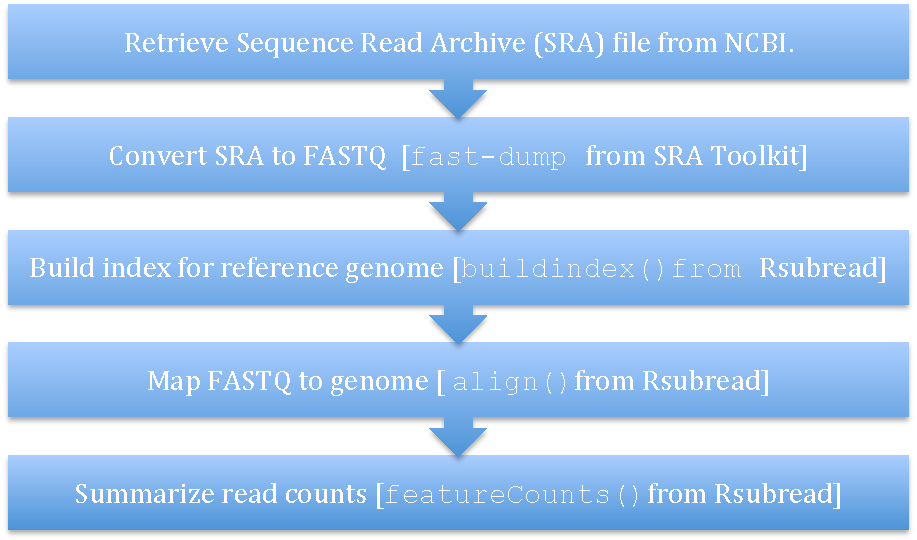
\includegraphics[width=0.7\linewidth]{Figures/flowchart.pdf}
	\caption{Work flow of data preprocessing: from raw reads sequencing data to read counts. Raw 
	data in this workflow are retrieved from the NCBI respository. Data processing is carried out 
	based on two softwares---the SRA Toolkit \citep{leinonen2010sequence} and the Rsubread aligner 
	\citep{liao2013subread}.}
	\label{fig:flowchart}
\end{figure}	



\subsubsection{Statistical issues}
The statistical analysis beginning from the read count matrix consists of three major parts: 1)
normalization---adjusting for sources of bias between samples; 2) differential expression (DE)
analysis---testing whether the expression levels of a gene are associated with treatment or 
experimental variables; 
and 3) gene set test---detecting which biological pathways are over-represented with DE genes.

\paragraph*{Normalization}
Despite the optimistic claim that RNA-Seq does not need sophisticated normalization
\citep{wang2009rna}, many works have shown that normalization of count data is highly desirable
 to account for various sources of bias between samples before accessing differential expression
\citep{anders2010differential,dillies2013comprehensive,hansen2012removing, risso2014nat,
	risso2011gc,robinson2010scaling}. Normalization is needed for adjusting differences in sequencing
depths or library sizes (total number of mapped reads for each biological sample) due to chance
variation in sample preparation. In DE analysis, gene expression levels are often estimated from
relative read frequencies. Therefore, normalization is also needed to account for the apparent
reduction or increase in relative read frequencies of non-differentially expressed genes simply to
accommodate the increased or decreased relative frequencies of truly DE genes. Currently there are
many normalization methods available, such as the trimmed mean of M-values (TMM) 
\citep{robinson2010scaling},
the DESeq normalization \citep{anders2010differential}, and remove unwanted variation (RUV)
\citep{risso2014nat}. 

\paragraph*{DE analysis}
Identification of DE genes is the key task in many gene expression studies. DE analysis uncovers the
association between expression levels of a gene and the covariates of interest. The covariates 
could either be
categorical (e.g., treatment/control status, cell types), or continuous (e.g., reagent
concentration, time). For example, to understand the effect of a drug, one might ask which genes are
\textit{up-regulated} (increased expression levels) or \textit{down-regulated} (decreased expression levels)
between treatment and control groups? Finding these genes will help researchers to understand the
cause of a disease and to develop effective medicine. In recent years, many statistical tools have 
been developed for DE detection (methods review can be found in 
\cite{rapaport2013comprehensive,seyednasrollah2015comparison,soneson2013comparison}) in RNA-Seq 
experiments. 
Most of those approaches are based on Poisson \citep{marioni2008rna, wang2010degseq}
or Negative Binomial (NB) distribution
\citep{anders2010differential,di2011nbp,oberg2012technical,robinson2007moderated, wu2013new} because
RNA-Seq expression data are present in the form of counts. %In practice, Poisson models are used
%when there are only technical replicates while NB models are more suitable when there are
%biological replicates.
The NB distribution based models are more popular for their flexibility to deal with 
\textit{over-dispersion} (a.k.a. extra-Poisson variation) that are often observed in RNA-Seq expression data.


%Prior to DE analysis, \textit{normalization} is needed to adjust for sources of bias (explained
%later). Depending on the question of interest, downstream analysis such as enrichment test of gene
%set or gene network analysis may also be performed. 
\paragraph*{Gene set test}
DE analysis evaluates each individual gene separately, but it fails to provide insights into
biological mechanisms since genes may be correlated and function together. %Therefore, people usually 
%examine an ensemble of genes. 
For this reason, \textit{gene set test} is a frequently used technique that enables
researchers to examine an ensemble of genes simultaneously and thus improves interpretability of DE
results. Gene set test is the assessment of
the association between a set of DE genes, which are significantly correlated with
treatment or experimental design variables, and a prior set of genes, which are biologically
related. Depending on the definition of the null hypothesis, there are two types of gene set test:
the \textit{self-contained} test and the \textit{competitive} test \citep{goeman2007analyzing}. A
self-contained test examines a set of genes by a fixed standard without reference to other genes in
the genome (see, for example, \cite{goeman2004global,goeman2005testing, huang2013gene,
	tsai2009multivariate, wu2010roast}). A competitive test compares DE
genes in the test set to those not in the test set
\citep{tian2005discovering,wu2012camera,yaari2013quantitative}. The competitive gene set test is
much more popular among genomic literatures \citep{gatti2010heading,goeman2007analyzing}.  




\subsubsection{Questions for this thesis}
In this thesis, we focus on three aspects of gene expression analysis: identifying stably
expressed genes from multiple RNA-Seq data sets (Chapter \ref{chap1}); estimating correlations
between test statistics via sample
correlations [NEED TO REVISE] (Chapter \ref{chap2}); and adjusting for correlations in competitive 
gene set test
(Chapter \ref{chap3}).

\paragraph{Identifying stably expressed genes}
Many of the current normalization methods, for example, TMM \citep{robinson2010scaling} and DESeq
\citep{anders2010differential} normalizations, assume that the majority of genes are not DE within
the experiment under investigation. However, this assumption could be violated for some experiments
where over $50\%$ of the genes' expression levels are altered by the treatments
\citep{loven2012revisiting, wu2013use}. The consequence with such assumption can be alleviated if
one could identify a set of stably expressed genes whose expression levels are stable across
different experimental conditions. This motivates us to identify such a set of genes by exploring a
large number of existing RNA-Seq data sets.

In microarray studies, there have been many attempts to find reference genes for normalization.
Traditionally, the \textit{house-keeping genes}  are used as reference genes.
However, a number of works have shown that house-keeping genes are not necessarily stably expressed
according to numerical stability measures (see, for example,
\cite{czechowski2005genome,huggett2005real}). Another choice, the \textit{spike-in genes}, is not
reliable for normalization due to the same issue \citep{risso2014nat}. A popular approach has been
to search from large sets of experiments for reference genes
\citep{czechowski2005genome,dekkers2012identification,frericks2008toolbox,gur2009identification,stamova2009identification}
whose expression stability are evaluated by some numerical stability measure. Validation experiments (e.g. reverse
transcription-PCR) show that reference genes identified by numerical methods generally outperform house-keeping genes or spike-in genes in terms of expression stability \citep{czechowski2005genome,hruz2011refgenes}.
We will follow the strategy of quantifying gene expression stability by numerical measures and
identify stably expressed genes.

Identifying stably expressed genes not only helps count normalization, but also improves
interpretability and comparability of RNA-Seq experiments in integrative analysis. Since genes are
measured by relative frequencies, we argue that DE is a relative concept: when a normalization
procedure is applied to a single data set, it effectively uses an implicit reference set of genes.
Furthermore, making the reference set explicit will be beneficial during DE analysis, because often times biologists compare results from one experiment to those from others experiments whose data are publicly
available. 

\paragraph{Estimating correlations of test statistics}
NEED SOMETHING HERE

\paragraph{Adjusting for correlations in competitive gene set test}
Competitive gene set test compares DE genes in the set against those in its complementary set. A
number of
statistical methodologies have been developed for this purpose (literature reviews can be found in
\cite{huang2009bioinformatics,khatri2012ten, mishra2014gene}). Broadly speaking, all of the
competitive gene set tests fall into two categories based on whether they assume independence of
expression profiles among genes. In earlier literatures, the inter-gene correlations were not taken
care of in the enrichment analysis procedure, such as \gent~\citep{tian2005discovering}, PAGE
\citep{kim2005page}, \genr~\citep{michaud2008integrative} or the $2\times 2$ contingency-table-based
tests \cite{alexa2010topgo, huang2007david,ye2006wego}. However, it has been argued that such test
procedures will result in inflated type I error 
\citep{efron2007testing,gatti2010heading,goeman2007analyzing,
	wu2012camera,yaari2013quantitative}, as genes within a gene set are often
co-expressed and function together.

Several approaches have been proposed to address inter-gene correlation problems in competitive gene
set test. One attempt is to evaluate the significance of the test set by permuting sample labels
\citep{efron2007testing,gatti2010heading,subramanian2005gene}. Sample permutation does not require
an explicit understanding of the underlying correlation structure among genes, and is therefore
supposed to protect the test against such correlations. One very famous example of this kind is the
\textit{gene set enrichment analysis} (GSEA) procedure \citep{subramanian2005gene}. Yet, sample
permutation method has been criticized for several reasons: first, it cannot be applied to
experiments having small
number of biological replicates (e.g., three samples each for a two-group comparison, which is common in RNA-Seq experiments);
second, it is computationally intensive since tens of thousands of DE tests are involved in each permutation; 
third, and most importantly, it implicitly alters the null hypothesis being tested and makes the null and
alternative difficult to be characterized \citep{goeman2007analyzing, khatri2012ten, wu2012camera}.
Another attempt has been to incorporate the inter-gene correlations into the formulation of gene set
test procedure \citep{wu2012camera,yaari2013quantitative}. CAMERA \citep{wu2012camera} estimates a
\textit{variance
	inflation factor} (VIF) from sample correlation (after the treatment effects removed), and then
includes it in its test statistic to assess the significance of the gene set. The same VIF has also 
been used by QuSAGE
\cite{yaari2013quantitative} 
to adjust for inter-gene correlations. However, accurate estimation of VIF relies on
the assumption that correlation between any two gene-level statistics are almost the same as
correlation between their corresponding expression levels. In Chapter \ref{chap2}, we will
demonstrate that this assumption is easily violated when differentially expressed genes are present,
and as a remedy, we will propose a new gene set test procedure in Chapter \ref{chap3}.  

\subsection{Statistical Methods}\label{subsec:glmm}
We have mentioned earlier that RNA-Seq data are essentially present in the form of count matrices. 
Therefore it might not be appropriate to impose normal distribution on gene expression profiles, 
especially when the sample size is small. Generalized linear models (GLMs) are a natural choice for 
analyzing RNA-Seq data. In addition, to account for random terms in biological experiments, GLMs 
are 
sometimes extended to generalized linear mixed models (GLMMs).
In this section, we will first describe the formulation GLMMs,
and then review commonly used methods for parameter estimation under this framework.

\subsubsection{Generalized linear mixed models}\label{subsubsec:intro-stat-framework}
GLMMs are a natural generalization of classical linear models. To illustrate this point, we will
begin with classical linear models, and discuss how to generalize them to linear mixed models and
then to GLMMs by relaxing different layers of assumptions. 
\paragraph{Classical linear models}\label{para:clm}
In a classical linear model, a vector $\bm y$ of $n$ observations is assumed to be a realization
of random variable $\bm Y$ whose components are identically distributed with mean $\bm \mu$. The
systematic part of this model is a specification of the mean $\bm\mu$ over a few unknown parameters
\citep{mccullagh1989generalized}. In the context of classical linear models, the mean is a function
of $p$ covariates $\bm X_1, \ldots, \bm X_p$,
\begin{equation}\label{eq:clm}
	\bm \mu =\beta_0 + \sum_{i=1}^p\beta_i \bm X_i
\end{equation}	
where $\beta$'s are unknown parameters and need to be estimated from data. For
$j$th %\footnote{Unless specified otherwise, we assume there are $n$ observations (i.e. $j=1, \ldots
%	,n$).} 
 observation $Y_j$, we specify $\epsilon_j$, a random term, to allow for measurement error.
Assuming a linear relationship between response $Y_j$ and predictors $(x_{1j}, \ldots, x_{pj})$, we
present the linear model 
\begin{equation}\label{eq:clm2}
	Y_j= \beta_0 + \beta_1x_{1j} + \ldots + \beta_p x_{pj} + \epsilon_j
\end{equation}
It is often required that $\epsilon_i$'s meet \textit{Gauss-Markov} assumption,
\begin{equation}\label{eq:gauss-markov}
	E(\epsilon_i)=0,~ \var[\epsilon_i]=
	\sigma^2<\infty, ~\cov[\epsilon_i, \epsilon_j]=0, \forall i \neq j.
\end{equation}
In practice, the error term is frequently, if not always, assumed to be normally distributed, 
\begin{equation}\label{eq:normalassumption}
	\bm \epsilon \sim N(0, \sigma^2 \bm I).
\end{equation}

\paragraph{Linear mixed models}\label{para:lmm}
The Gauss-Markov assumption in equation (\ref{eq:gauss-markov}) is vulnerable in practice, for 
example,
nonconstant variance, or correlated data where Cov$[\epsilon_i, \epsilon_j]\neq 0$.
Equation (\ref{eq:clm2}) in either case, without loss of generality, can be expressed in matrix
form as
\begin{equation}\label{eq:clm3}
	\bm Y = \bm {X\beta} + \bm \epsilon, ~ E[\bm \epsilon] = \bm 0, ~\cov[\bm\epsilon] = \bm V
\end{equation}
where $\bm V$ is a known positive definite matrix. Let $\bm Y^{\ast} = \bm V^{-1/2}\bm Y = \bm
V^{-1/2}\bm {X\beta} + \bm V^{-1/2}\bm \epsilon$. It follows that Cov$(\bm Y^{\ast})= \bm I$ and the
techniques in classical linear models are readily applicable to estimate $\bm \beta$. However, this
method relies on the assumption that $\bm V$ is known which is rarely, if ever, given. On the other
hand, the structure of $\bm V$, which depends on experiment setup, can often be specified by a few
unknown parameters. 

Nonindependence can occur in the form of serial correlation or cluster correlation
\citep[chapter~17]{rencher2008linear}. Serial correlation usually exists in experiments with
repeated measurements---multiple measurements taken from a response variable on the same
experimental unit. Several covariance structures are available for implementation (for more details,
see \citet[chapter~5]{littell2006sas}).  Cluster correlation is present when measurements of a
response variable are grouped in some way. In many situations, the covariance of cluster correlated
data can be specified using an extension of standard linear model by 
\begin{equation}\label{eq:lmm}
	\bm Y = \bm {X\beta} + \bm {Z_1u_1}+\cdots + \bm {Z_qu_q} + \bm \epsilon	
\end{equation}
equation (\ref{eq:lmm}) differs from equation~(\ref{eq:clm3}) only in the $\bm {Z_iu_i}$ terms,
which is the key part of \textit{linear mixed models}.  The $\bm Z_i$  are known $n\times p_i$ full
rank matrices, usually used to specify membership of predictors in various subgroups. The most
important innovation in this model is that instead of estimating $\bm u_i$'s as fixed parameters, we
assume them to be unknown random quantities, and $E[\bm u_i]=0$, $\cov[\bm u_i]= \sigma_i^2 \bm
I_{p_i}$ for $i=1, \ldots, q$. It is, in many cases, reasonable to require that $\bm u_i$ are
mutually independent, and that $\bm u_i$ is independent of $\bm \epsilon$ for $i=1, \ldots, q$. If
we further impose normal distribution on the random terms and errors, then equation (\ref{eq:lmm})
can be casted in a Bayesian framework,
\begin{equation}\label{eq:lmmGuass}
	\begin{split}
		\bm y|\bm u_1, \ldots, \bm u_q   & \sim  N_n(\bm {X\beta} + \sum_{i=1}^q \bm {Z_iu_i}, \sigma^2\bm
		I_n),  \\
		\bm u_i &\sim N_{p_i}(0, \sigma_i^2 \bm I_{p_i}).
	\end{split}
\end{equation}
The modeling issues are: (a) estimation of variance components $\sigma_i^2$ and $\sigma^2$; (b)
estimation of random effects $u_i$ if needed. For the variance component estimation, there are
primarily three approaches: (i) procedures based on expected mean squares from analysis of variance
(ANOVA); (ii) maximum likelihood (ML); and (iii) restricted/residual maximum likelihood (REML). For
more details, see \citet[Chapter 1]{littell2006sas}.


\paragraph{Generalized linear models}\label{para:glm}

We can take a different perspective of classical linear models by arranging equations
(\ref{eq:clm})--(\ref{eq:gauss-markov}) into three parts, following the notations of \citet[Chapter
2]{mccullagh1989generalized}, 
\begin{enumerate}
	\item[(i)] the \textit{random component} $Y_j$ has constant variance $\sigma^2$ and
	%	\begin{equation}\label{eq:part1}
	$E[ Y_j]= \mu_j$.
	%		\end{equation}
	\item[(ii)] the \textit{systematic component}---the linear predictor $\eta_j$ is modeled by
	covariates $\bm x_j =: x_{1j},\ldots, x_{pj}$, 
	\begin{equation}\label{eq:part2}
		\eta_j = \sum_{i=1}^p\beta_i x_{ij}=\bm {x_j\beta}.
	\end{equation}
	\item[(iii)] the \textit{link function} relates the random components and the systematic
	components by 
	\begin{equation}\label{eq:part3}
		\eta_j = g(\mu_j).
	\end{equation}
\end{enumerate}
The classical linear models fits within this framework if we assume that the random components 
$Y_j$'s
are independent and normally distributed, and that the link function is identity (i.e., $g(\mu_j)=
\mu_j$).

We can extend part (i)---by allowing $Y_j$ to come from an exponential family (e.g., Poisson,
Gamma or Binomial distribution), and part (iii)--- by requiring the link function to be monotonic
differentiable (e.g., $g(\mu_j)= \log \mu_j$). These two extensions lead to the
\textit{generalized linear models} (GLMs), a framework that is especially suitable when a normal 
distribution is no longer appropriate to be assumed on the response. 

\paragraph{Generalized linear mixed models}\label{para:glmm}
Generalized linear mixed models (GLMMs) is a further extension of GLMs that incorporates random
components into part (ii), represented in a matrix notation
\begin{equation}\label{eq:q5}
	\bm \eta = \bm {X\beta} + \sum_{i=1}^q\bm {Z_iu_i}
\end{equation}
where  $\bm Z_i$ and $\bm u_i$ are specified in equation (\ref{eq:lmm}). 

To formally present GLMMs, we start with the conditional distribution of $\bm y$ given $\bm u$. It
is typical to assume that vector $\bm y$ consists of conditionally independent elements, each coming
from the exponential family (or similar to the exponential family), 
\begin{equation}\label{eq:glmm}
	\begin{split}
		y_j|\bm u & \sim \text{~indep.~} f_{Y_j |\bm u} (y_j|\bm u), \\
		f_{Y_j|u}(y_j; \theta, \phi|\bm u) &= \exp \left[ \frac{y_j\theta_j	 -b(\theta_j)}{a_j(\phi)}
		+ c(y_i, \phi)\right].
	\end{split}
\end{equation}	
It can be verified that the conditional mean of $y_j$ is related to $\theta_j$ in equation
(\ref{eq:glmm}) by the identity $\mu_j = \partial b(\theta_j)/\partial \theta_j$. The transformation
of the mean allows us to model the fixed and the random factors by a linear model
\begin{equation}\label{eq:glmm2}
	\begin{split}
		E[y_j|\bm u] &= \mu_j,\\
		g(\mu_j) = \eta_j &= \bm X_j\bm \beta + \bm Z_j\bm u.
	\end{split}
\end{equation}
Finally, we assign a distribution to the random effects
\begin{equation}
	\bm U \sim \phi_{\bm U}(\bm u),
\end{equation}
which completes the specification of GLMMs. It is often, if not always, assumed that $\bm u$ come
from a normal distribution.

\paragraph{An example---Poisson log-linear mixed-effect model}\label{poisson} 
We will illustrate one specific type of GLMMs---the Poisson log-linear mixed-effect model in the 
context of RNA-seq experiments. Suppose we have RNA-Seq expression profiles (in the form of 
counts)
randomly selected from three experiments conducted in three different labs. For each experiment, 
there are two treatments and two biological replicates for each treatment. We are not interested in 
the specific levels of treatment, but focus
more on the overall variation of treatments. In this sense, the treatment effects are also
considered as random. For a single gene, let $Y_{jkl}\sim \text{Poisson}(\mu_{jkl})$ be the read
count for $j$th biological sample from $k$th treatment of $l$th experiment. The link function
$\eta_{jkl} = \log (\mu_{jkl})$ relates the mean $\mu_{jkl}$ to the linear predictors by equation
(\ref{eq:glmm2})  
\begin{equation}\label{eq:example}
	\log (\mu_{jkl}) = \log (N_{jkl}R_{jkl}) + \xi + a_{j} + b_{k(j)} + \epsilon_{jkl},
\end{equation}
where $N_{jkl}R_{jkl}$ is the normalized library size (total number of read counts mapped to the
genome),  $j=1, 2,  3$, $k=1, 2$ and $l=1, 2$; the random terms $a_j \sim N(0, \sigma_1^2), 
b_{k(j)}\sim N(0,\sigma_2^2)$ and $\epsilon_{jkl}\sim N(0, \sigma_0^2)$ represent the experimental, 
treatment and sample effects respectively, and are mutually independent. If
the observations are sorted by experiment and then by treatment nested in experiment, we can present
the model in the form of equation~(\ref{eq:q5}), with  $\bm \beta = (\log [N_{111}R_{111}]  +
\xi,\ldots, \log [N_{223}R_{223}]  + \xi)^T, ~\bm u = (\bm a, \bm b, \bm \epsilon)$ and 
\[
q = 2,  \bm X = \left[
\begin{array}{c}
1\\
1\\
1\\
1\\
1\\
1\\
1\\
1\\
1\\
1\\
1\\
1\\
\end{array}
\right],
\bm Z_1=\left[
\begin{array}{ccc}
1 & 0 & 0 \\
1 & 0 & 0 \\
1 & 0 & 0 \\
1 & 0 & 0 \\
0 & 1 & 0 \\
0 & 1 & 0 \\
0 & 1 & 0 \\
0 & 1 & 0 \\
0 & 0 & 1 \\
0 & 0 & 1 \\
0 & 0 & 1 \\
0 & 0 & 1 \\
\end{array}
\right],
\bm Z_2=\left[
\begin{array}{cccccc}
1 & 0 & 0  & 0 & 0  &0\\
1 & 0 & 0  & 0 & 0  &0\\
0 & 1 & 0  & 0 & 0  &0\\
0 & 1 & 0  & 0 & 0  &0\\
0 & 0 & 1  & 0 & 0  &0\\
0 & 0 & 1  & 0 & 0  &0\\
0 & 0 & 0  & 1 & 0  &0\\
0 & 0 & 0  & 1 & 0  &0\\
0 & 0 & 0  & 0 & 1  &0\\
0 & 0 & 0  & 0 & 1  &0\\
0 & 0 & 0  & 0 & 0  &1\\
0 & 0 & 0  & 0 & 0  &1\\
\end{array}
\right], \bm Z_3 = \bm I_{12}.
\]
Then it follows that 
\[\bm\Sigma = \sigma_1^2\bm{Z_1Z_1'} + \sigma_2^2\bm{Z_2Z_2'} + \sigma_0^2\bm I_{12}=
\left[
\begin{array}{ccc}
\bm\Sigma_d  & \bm O  &\bm O\\
\bm O & \bm\Sigma_d  & \bm O \\
\bm O  &\bm O   & \bm\Sigma_d\\
\end{array}
\right],\]
where $\bm O$ is a $4\times 4$ matrix of 0 and 
\[
\bm \Sigma_d = \left[
\begin{array}{cccc}
\sigma^2_1+ \sigma^2_2 + \sigma^2_0  & \sigma^2_1+\sigma^2_2 & \sigma^2_1 &\sigma^2_1\\
\sigma^2_1+\sigma^2_2 & \sigma^2_1 +\sigma^2_2 +\sigma^2_0 &\sigma^2_1 &\sigma^2_1\\
\sigma^2_1 & \sigma^2_1& \sigma^2_1+\sigma^2_2+\sigma^2_3 & \sigma^2_1 + \sigma^2_2\\
\sigma^2_1 &\sigma^2_2 &\sigma^2_1 +\sigma^2_2 & \sigma^2_1 +\sigma^2_2 +\sigma^2_0\\
\end{array}
\right]
\]
%What is different between LMM and GLMM is that the response variable can come from other
%distributions besides gaussian.
The challenge due to the complexity of GLMM is the estimation of parameters. In the next section,
we will summarize current available methods for estimating parameters and variance components.

\subsubsection{Estimation of generalized linear mixed models}\label{subsub:estimation}	
There are three general approaches for estimating parameters under GLMM settings \citep[Chapter
7]{myers2012generalized}: (i) using numerical method to approximate the integrals for the likelihood
functions and obtaining the estimating equations; (ii) linearization of the conditional mean and
then iteratively applying linear mixed model techniques to the approximated model; (iii) Bayesian
approach.  
%There are several methods: Maximum Likelihood,  Generalized estimating equations, penalized
%quasi-likelihood \citep{breslow1993approximate}, conditional likelihood...  etc. see \cite[Chapter
%8]{mcculloch2001generalized} In this chapter, we mainly discuss the first approach, in that (ii) is
%found to be biased especially when sample size is small \citep[Chapter 7]{myers2012generalized} and
%(iii) is computationally intensive.

In the following discussion, we assume conditional distribution of $\bm Y$ given $\bm u$ is
$f_{Y}(\bm y|\bm \beta, \bm u)$, the link function is $\bm \eta = g(\bm \mu)$, and $\bm \eta$
relates the covariates by equation (\ref{eq:glmm2}). We also assume that the random term $\bm u$ 
have some distribution $\bm U \sim \phi_{\bm U}(\bm u|\bm \Sigma)$. 	

\paragraph{Likelihood function approach}\label{para:likelihood-approach}
It is straightforward  to write down the likelihood function of $\bm Y$ by first obtaining the
joint likelihood of $(\bm Y, \bm u)$ and then integrating out the random term $\bm u$,
\begin{equation}\label{eq:joint-likelihood}
	L(\bm Y|\bm\beta, \bm \Sigma) = \int f(\bm y|\bm \beta, \bm u)\phi(\bm u|\bm \Sigma)d \bm u.
\end{equation}
A major challenge in estimating GLMMs is the integration in equation (\ref{eq:joint-likelihood})
over the $n$-dimensional distribution of $\bm u$. Numerical approximation are usually used in
evaluating the integral. In this part we will discuss the \textit{Gauss-Hermite} (GH) quadrature
which is recognized as a higher order Laplace approximation \citep{liu1994note}.
Gauss-Hermite quadrature is used for integrals of the form 
$\int_{-\infty}^{\infty}f(x) e^{-x^2}dx$ that can be approximated by a weighted sum of  $f(x)$:
\begin{equation}\label{eq:gh2}
	\int_{-\infty}^{\infty}f(x) e^{-x^2}dx \approx \sum_{i=1}^m w_if(x_i)
\end{equation}
In equation (\ref{eq:gh2}), $x_i$'s are the zeros of $m$th order Hermite polynomial 
\[H_m(x) = (-1)^m\exp(\dfrac{x^2}{2})\frac{d^m}{dx^m}\exp(-\dfrac{x^2}{2})\]
and $w_i$ are the corresponding weights. For a Hermite polynomial of degree $m$, $x_i$ and $w_i$
can be calculated as 	
\begin{equation}\label{eq:gh3}
	x_i = i\text{th zero of } H_m(x),~~  w_i = \frac{2^{m-1}m!\sqrt{\pi}}{m^2[H_{m-1}(x_i)]^2}. 
\end{equation}
Equation (\ref{eq:gh2}) gives the exact numerical value for all polynomials up to degree of
$2m-1$. 
An improved version of the regular Gauss-Hermite quadrature is to center and scale the quadrature
points  by the empirical Bayes estimate of the random effects and the Hessian matrix from the Bayes
estimate suboptimization \citep{liu1994note}. This procedure is called \textit{Adaptive
	Gauss-Hermite} (AGH) quadrature \citep{pinheiro1995approximations}. %We illustrate AGH by the
%example of RNA-Seq study mentioned in \textbf{section \ref{poisson}}.\\

%Let $f(\bm Y|\bm \beta, \bm u)=\text{Pois} (\bm \eta)$ where $\bm \eta$ is defined by (\ref{q5})
%and  $\phi(\bm u|\bm \Sigma)=N(\bm 0, \bm \Sigma)$.  
The AGH quadrature starts with maximizing the integrand $h(\bm u|\bm y, \bm \beta, \bm \Sigma) :=$ 
\\$f(\bm y|\bm \beta, \bm u)\phi(\bm u|\bm \Sigma)$ in equation (\ref{eq:joint-likelihood}) with
respect to the random term $\bm u$. The resulting estimate $\hat{\bm u}^{(n)}$ at iteration $n$ is
the joint posterior modes for the random effects. Because $\bm \beta$ and $\bm \Sigma$ are unknown,
they are replaced by the current estimates $\hat{\bm \beta}^{(n)}$ and $\hat{\bm \Sigma}^{(n)}$. The
Hessian matrix $\hat{\bm H}^{(n)}$ can be obtained by evaluating the second order partial
derivatives of $\log(h(\bm u|\bm y, \hat{\bm \beta}^{(n)}, \hat{\bm \Sigma}^{(n)}))$ at $\hat{\bm
	u}^{(n)}$. Consequently, $\hat{\bm \Omega}^{(n)} =-\hat{\bm H}^{(n)} $ is the estimated covariance
matrix for the random effects posterior modes. It follows from equation (\ref{eq:joint-likelihood})
that for the $i$th cluster 
\begin{equation}\label{eeq:clm.3.1}
	L( \bm Y_i|\bm \beta, \bm \Sigma) = \int f(\bm y_i|\bm \beta, \bm u )\phi(\bm u|\bm\Sigma)d\bm u =
	\int \frac{f(\bm y_i|\bm \beta, \bm u )\phi(\bm u|\bm\Sigma)}{\phi(\bm u|\hat{\bm
			u}^{(n)},\hat{\bm \Omega}^{(n)} )}\phi(\bm u|\hat{\bm u}^{(n)},\hat{\bm \Omega}^{(n)} )d\bm u
\end{equation}
%[copied from SAS help] 
Let $m$ be the number of quadrature points (i.e., the order of the Hermite
polynomial) in each dimension for each random effect term, and $Q$ the number of random
effects. If $\bm x = (x_1, \ldots, x_m)$ are the nodes for standard Gauss-Hermite quadrature, and
$\bm x^{\ast}_j=(x_{j_1}, \ldots, x_{j_Q}) $ is a point on the $Q$ dimensional quadrature grid, then
the centered and scaled nodes are 
\begin{equation}\label{1.3.2}
	\bm  a_j^{\ast} = \hat{\bm u}^{(n)} + \sqrt{2} [\hat{\bm \Omega}^{(n)} ]^{1/2}\bm x^{\ast}_j
\end{equation}
The centered and scaled nodes, along with the Gauss-Hermite quadrature weights $\bm w = (w_1,
\ldots, w_m)$ are used to construct the $Q$ dimensional integral of equation (\ref{eeq:clm.3.1}),
approximated by 
\begin{equation}\label{eq:gh-approx}
	\begin{aligned}
		L(\bm y_i|\bm\beta, \bm \Sigma) &\approx\sum_{j_1=1}^m\cdots \sum_{j_Q=1}^m\frac{f(\bm y_i|\bm
			\beta, \bm  a_j^{\ast})\phi(\bm  a_j^{\ast}|\bm\Sigma)}{\phi(\bm  a_j^{\ast}|\hat{\bm
				u}^{(n)},\hat{\bm \Omega}^{(n)} )}w_{j_1}\cdots w_{j_Q}\\
		& = (2)^{Q/2}|\hat{\bm \Omega}^{(n)}|^{1/2}\sum_{j_1=1}^m\cdots \sum_{j_Q=1}^m\left[ f(\bm y_i|\bm
		\beta, \bm  a_j^{\ast} )\phi(\bm  a_j^{\ast}|\bm\Sigma) 
		\prod_{k=1}^Qw_{jk}\exp(x_{jk}^2)\right].
	\end{aligned}
\end{equation}
Thus the multidimensional unbounded integral is approximated by a finite summations. Now that the
likelihood has the form of equation (\ref{eq:gh-approx}), a number of numerical methods (e.g. 
Newton-Raphson
or Fisher's scoring) can be used to estimate $(\bm \beta,  \bm \Sigma)$. 

It should be noted, however, as the number of dimension $Q$ increases, the computational burden for
approximating equation (\ref{eq:gh-approx}) grows exponentially since the total number of nodes is 
$m^Q$. 
Therefore it is difficult to implement AGH procedure with more than three random effects
\citep{bolker2009generalized}.


\paragraph{Estimation based on linearization}\label{para:linearization}

%\url{http://support.sas.com/documentation/cdl/en/statug/63033/HTML/default/viewer.htm#statug_glimmix_a0000001425.htm}

%Under the linearization framework, the GLMM is approximated by a linear mixed model based on
%current values of the covariance parameter estimates. The resulting linear mixed model is then fit,
%which is itself an iterative process. The process of linear approximation must be repeated several
%times until some convergence criterion is met. Upon convergence, the new parameter estimates are
%used to update the linearization, which results in a new linear mixed model. 
%{\large maybe a brief introduction}

Under GLMM framework, we have some conditional distribution of $\bm Y$ given $\bm u$. Without loss
of generality, we assume
\begin{equation}\label{eq:linearization1}
	\begin{aligned}
		E[\bm Y|\bm u] &= \bm \mu = g^{-1}(\bm \eta) = g^{-1}(\bm{X\beta} + \bm {Zu}), \\
		\text{Var}[\bm Y|\bm u]  & = \bm S,
	\end{aligned}
\end{equation}
where $\bm u \sim N(\bm 0, \bm \Sigma)$.  The linearization is done by Taylor expansion of equation
(\ref{eq:linearization1}) about estimates $\bm \eta$. Two approaches proposed by \citet{breslow1993approximate}---the
\textit{penalized quasi-likelihood } (PQL) and the \textit{marginal quasi-likelihood} (MQL)---may be used
for this purpose. 

\subparagraph*{Penalized Quasi-likelihood}
The PQL procedure uses a first order Taylor expansion of $\bm \beta$ and $\bm u$, at $\tilde{\bm
	\beta} $ and $ \tilde{\bm u} $, respectively
\begin{equation}\label{eq:linearization2}
	g^{-1}(\bm\eta) \approx g^{-1}(\hat{\bm \eta}) + \tilde{\bm \Omega}_{PQL}(\bm \eta-\tilde{\bm
		\eta}),
\end{equation} 
where $\tilde{\bm \Omega}_{PQL}$ is an $n\times n$ diagonal matrix whose $(i, i)$ entry is 
$\partial {g^{-1}(\bm \eta_i)}/\partial \bm \eta_i $ evaluated at $\tilde{\bm \eta}= \bm X\tilde{\bm
	\beta} + \bm Z\tilde{\bm u}$. Multiplying both sides by $\bm \tilde{\bm\Omega}_{PQL}^{-1}$,
equation
(\ref{eq:linearization2}) can be rearranged as 
\begin{equation}\label{eq:linearization3}
	\bm {X\beta} + \bm {Zu} \approx \tilde{\bm \Omega}_{PQL}^{-1}[g^{-1}(\bm\eta)- g^{-1}(\tilde{\bm
		\eta})]  + \bm{X}\tilde{\bm \beta} + \bm Z\tilde{\bm u}.
\end{equation}
Note that the right hand side of equation (\ref{eq:linearization3}) is just the expected value,
conditioning on $\tilde{\bm \beta}$ and $\tilde{\bm u}$, of the pseudo-response 
\begin{equation}\label{se4}
	\tilde{\bm Y }=\tilde{\bm \Omega}_{PQL}^{-1}[\bm Y- g^{-1}(\tilde{\bm \eta})]  + \bm{X}\tilde{\bm
		\beta} + \bm Z\tilde{\bm u},
\end{equation}
whose variance-covariance matrix given $\bm u$ is 
\begin{equation}\label{se5}
	\text{Var}[\tilde{\bm Y }|\bm u] =\tilde{\bm \Omega}_{PQL}^{-1} \text{Var}[\bm Y|\bm u]\tilde{\bm
		\Omega}_{PQL}^{-1} = 
	\tilde{\bm \Omega}_{PQL}^{-1} \bm S \tilde{\bm \Omega}_{PQL}^{-1}.
\end{equation}
Then we can consider the model 
\begin{equation}\label{se6}
	\tilde{\bm Y } = \bm{X\beta} + \bm {Zu}  + \bm \epsilon
\end{equation}
which is a linear mixed model with pseudo response $\tilde{\bm Y }$ with covariance matrix 
\begin{equation}
	\bm W = \text{Var}[ \tilde{\bm Y } |\bm u] = \bm{Z\Sigma Z'} + \tilde{\bm \Omega}_{PQL}^{-1} \bm S
	\tilde{\bm \Omega}_{PQL}^{-1}.
\end{equation}
Model (\ref{se6})  has exactly the same form as the linear mixed models (see Section 
\ref{para:lmm}),
except that an estimate of $(\bm\beta, \bm u)$  is needed for calculating the pseudo-response
$\tilde{\bm Y }$ in equation (\ref{se4}). An iterative procedure can be used to estimate the
parameters in model (\ref{se6}) by substituting raw data $\bm y$ for $\tilde{\bm y}$  and identity
matrix $\bm I$ for $\bm S$ as starting values. Techniques for fitting LMM such as REML can be
readily applied to estimate variance components $\bm \Sigma$, upon which $\hat{\bm W}$ is
calculated. The estimate for $\bm \beta$ is given by
\begin{equation}
	\hat{\bm\beta} = (\bm X^T\hat{\bm W}^{-1} \bm X)^{-1}\bm X^T\hat{\bm W}^{-1}\bm X \tilde{\bm y},
\end{equation}
and the estimate for random effect is 
\begin{equation}\label{se7}
	\hat{\bm u} = \hat{\bm\Sigma } \bm Z \hat{\bm W}^{-1} (\tilde{\bm y}-\bm {X} \hat{\bm \beta}).
\end{equation}
Then the pseudo-response is updated and the procedure is repeated until convergence is reached for
fixed effects and variance components.  Note that equation (\ref{se7}) estimates a vector of random
effect. For this reason, PQL is also referred to as \textit{subject-specific} estimate procedure. 

\subparagraph*{Marginal Quasi-likelihood} 
One of the motivation for MQL is that usually one is more interested in estimating the marginal
mean of the response than estimating the conditional mean as is done by equation (\ref{se7}) in
PQL. Since $E[\bm \eta|\bm u]= \bm {X\beta} + \bm {Zu}$, the unconditional mean is $E[\bm \eta] =
E[E(\bm \eta|\bm u)]= \bm {X\beta}$. A first-order Taylor expansion of $E[\bm Y|\bm u]$ about $\bm X
\bm\beta$ is given by 
\begin{equation}\label{se8}
	E[\bm Y|\bm u] = g^{-1}(\bm \eta) \approx g^{-1} (\bm{X\beta}) + \tilde{\bm \Omega}_{MQL} (\bm
	\eta - \bm X\bm \beta)
\end{equation}
where $\tilde{\bm \Omega}_{MQL}$ is evaluated at $\bm {X\beta}$ (recall that for PQL, $\tilde{\bm
	\Omega}_{PQL}$ is evaluated at $\bm {X\beta} + \bm {Zu}$). The unconditional expected value of 
$\bm
Y$ is approximately $g^{-1}(\bm {X\beta})$ by equation (\ref{se8}). The variance of $\bm Y$ can then
be derived from the relation $\text{Var}(\bm Y)= E[\text{Var}(\bm Y|\bm u)] + \text{Var}[E(\bm Y|
\bm u)]$, which yields
\begin{equation}\label{se9}
	\text{Var}[\bm Y] = \tilde{\bm \Omega}_{MQL} \bm {Z\Sigma Z'}\tilde{\bm \Omega}'_{MQL} + \bm
	S_{\bm \eta_0}.
\end{equation}
A linearization performed at $\bm \eta_0= \bm X \bm \beta_0$ leads to 
\begin{equation}\label{se9.1}
	g^{-1}(\bm \eta) \approx g^{-1} (\bm{X\beta_0}) + \tilde{\bm \Omega}_{MQL} (\bm \eta - \bm X\bm
	\beta_0),
\end{equation}
and multiplying both sides by $\tilde{\bm \Omega}_{MQL} ^{-1}$, equation (\ref{se9.1}) then can be
arranged to 
\begin{equation}
\bm {X\beta} + \bm {Zu} \approx \tilde{\bm \Omega}_{MQL}^{-1}[g^{-1}(\bm\eta)- g^{-1}(\bm
\eta_0)]  + \bm{X}\bm \beta_0. 
\end{equation}
Defining the pseudo-response $\tilde{\bm Y}_{MQL}$ as
\begin{equation}\label{se10}
	\tilde{\bm Y}_{MQL} =  \tilde{\bm \Omega}_{MQL}^{-1}[\bm Y- g^{-1}(\bm \eta_0)]  + \bm{X}\bm
	\beta_0,  
\end{equation}
we next consider the linear mixed model 
\[ \tilde{\bm Y}_{MQL}  = \bm {X\beta}+ \bm {Zu}  + \bm \epsilon, \] 
where $\text{Var}(\bm \epsilon) $ is given by equation (\ref{se9}).  The estimating procedure for
fixed effect parameter $\bm \beta$ and variance component $\bm \Sigma$ is the same as those in the 
PQL approach.
Note that the pseudo-response is not a function of $\bm u$ any more, so updating this quantity does
not require calculating the random effects $\bm u$. Accordingly, the MQL approach is also referred 
to as \textit{population-averaged} estimate approach.

\citet{breslow1995bias}  and \citet{pinheiro2006efficient} point out that PQL approach may lead to
asymptotically biased estimates and hence to inconsistency. It is not recommended to use simple PQL
method in practice. 


\paragraph{Bayes approach}
As mentioned earlier, for models with higher dimensional integrals, it is not practical to
evaluate the likelihood function by AGH procedure. For mixed models, a typical strategy is to treat
the random effects to be missing data. Following this idea, the problem of estimating variance
components associated with random effects can be simplified. Denote the \textit{complete data} as
$\bm v = (\bm y, \bm u)$, the log-likelihood of $\bm v$ can be expressed as 
\begin{equation}\label{eq:bayes}
	\log \pi(\bm \beta , \bm \Sigma|\bm v) = \log f(\bm y|\bm \beta, \bm u) + \log \phi(\bm u|\bm
	\Sigma)
\end{equation}  
The optimal solution for parameters in equation (\ref{eq:bayes}) can be obtained by
\textit{expectation-maximization} (EM) algorithm. The EM algorithm consists of two steps, readily 
implemented as follows:
\begin{enumerate}
	\item \textbf{E-Step}. At $(k+1)$th iteration given $\bm \beta^{(k)}$ and $\bm\Sigma^{(k)}$,  
	calculate 
	\begin{equation}\label{eq:bayes-em}
		\begin{aligned}
			E_{\bm \beta^{(k)}}[\log f(\bm \beta , \bm \Sigma|\bm v)|\bm y]&= Q_1(\bm \beta, \bm 
			\beta^{(k)}),\\
			E_{\bm \Sigma^{(k)}}[\log \phi(\bm \Sigma|\bm v)|\bm y]&= Q_2(\bm \Sigma, \bm 
			\Sigma^{(k)}).
		\end{aligned}
	\end{equation}
	\item \textbf{M-Step}. Maximize $Q_1$ and $Q_2$ to update  $\bm \beta^{(k+1)}$ and
	$\bm\Sigma^{(k+1)}$.
\end{enumerate}
The \textbf{E} and \textbf{M} steps are alternated until convergence is reached. Unfortunately, the
expectations in equation (\ref{eq:bayes-em}) cannot be computed in closed form for GLMMs. However,
they may be approximated by \textit{Markov chain Monte Carlo} (MCMC). In light of this,
\citet{mcculloch1997maximum} developed a Monte Carlo EM (MCEM) algorithm. 

The Metropolis-Hastings algorithm is used for drawing samples from difficult-to-calculate density 
functions.
For Metropolis algorithm, a proposal distribution $g(\bm u)$ is selected, from which an initial
value of $\bm u$ is drawn. The new candidate value $\bm u' = (u_1, u_2, \ldots,u_{k-1}, u_k',
u_{k+1}, \ldots, u_Q)$, which has all elements the same as previous values expect the $k$th,   is
accepted (as opposed to keeping the previous value) with probability
\begin{equation}\label{eq:metropolis}
	A_k(\bm u', \bm u) = \min \left\{1, ~\frac{f(\bm u'|\bm y, \bm \beta, \bm \Sigma)g(\bm u)}{f(\bm
		u|\bm y, \bm \beta, \bm \Sigma)g(\bm u')}\right\}.
\end{equation}
If we choose $g(\bm u) = \phi (\bm u|\bm\Sigma)$, the ratio term in equation (\ref{eq:metropolis})
can be simplified to 
\begin{equation}\label{eq2.3.4}
	\begin{aligned}
		& ~~~~\frac{f(\bm u'|\bm y, \bm \beta, \bm \Sigma)g(\bm u)}{f(\bm u|\bm y, \bm \beta, \bm
			\Sigma)g(\bm u')} \\
		& = \left[\frac{f(\bm u', \bm y| \bm \beta, \bm \Sigma)}{f(\bm y| \bm \beta, \bm \Sigma)}\phi (\bm
		u|\bm\Sigma)\right]  \Biggm/ \left[
		\frac{f(\bm u, \bm y|\bm \beta, \bm \Sigma)}{f(\bm y|\bm \beta, \bm \Sigma)}\phi (\bm
		u'|\bm\Sigma)\right]\\
		& = \frac{f(\bm y|\bm u', \bm \beta, \bm \Sigma)\phi (\bm u'|\bm\Sigma)\phi (\bm
			u|\bm\Sigma)}{f(\bm y|\bm u, \bm \beta, \bm \Sigma)\phi (\bm u|\bm\Sigma)\phi (\bm u'|\bm\Sigma)}\\
		& = \frac{f(\bm y|\bm u', \bm \beta, \bm \Sigma)}{f(\bm y|\bm u, \bm \beta, \bm \Sigma)}
	\end{aligned}
\end{equation}
The MCEM procedure combines the EM steps and Metropolis algorithm in estimating the fixed
parameters and variance components, summarized as follows:
\begin{enumerate}
	\item Choose the starting value of $\bm \beta^{(0)}, \bm \Sigma^{(0)}$. Set $b= 0$
	\item Generate the sequence $\bm u^{(1)}, \bm u^{(2)}, \ldots, \bm u^{(B)}$ from the conditional
	distribution of $\bm u$ given $y$ with Metropolis algorithm.
	\item Maximize $\sum_{b=1}^B \log f(\bm y|\bm u^{(b)}, \bm\beta)/B$ and $\sum_{b=1}^B\log\phi(\bm
	u^{(b)}|\bm \Sigma)/B$ to obtain $\bm \beta^{(m+1)}$ and $\bm\Sigma^{(m+1)}$
	\item Iterate between step 2 and 3 until convergence is reached.
\end{enumerate}
This method can be easily extended to allow for multiple random effects. Yet the advantage comes
at a price. A major drawback of MCEM is the computational intensity.  First, the convergence of $EM$
algorithm is usually very slow, especially at the neighborhood of maximum of marginal likelihood.
Second, the chain in Metropolis algorithm has to run long enough for reliable estimation. 

In the Bayes framework, there are other alternatives to estimate the parameters and variance
components, for example,  \textit{Monte Carlo Newton-Raphson} (MCNR) \citep{mcculloch1997maximum} and  MCMC \citep{hadfield2010mcmc}.

\paragraph{Example of estimating parameters}
We will demonstrate the estimating procedure with the Poisson log-linear mixed-effect model
discussed in Section \ref{subsubsec:intro-stat-framework}.
The estimation procedure starts from the joint density function of $\bm Y=(Y_{jkl})'$ given $\bm
\mu= (\mu_{jkl})'$,
\begin{equation}\label{eq:poisdens}
	f(\bm y|\bm \mu )=\prod_{ j,
		k,l}f(y_{jkl}|\mu_{jkl})=\prod_{j,k,l}\frac{[\mu_{jkl}]^{y_{jkl}}\exp(-\mu_{jkl})}{y_{jkl}!}.
\end{equation}
A re-expression of  equation (\ref{eq:example}) in matrix form gives 
\[\log\bm \mu= \bm {X\beta} + \bm {Z_1 a} + \bm{Z_2b} + \bm I_{12}\bm \epsilon. \]
%	where $\bm \xi = \bm 1\cdot\xi$ and $\bm 1$ is a vector of 1s, $\bm Z_1$ is the design matrix for
%random effects $\bm \alpha=(\alpha_l)$, and $\bm Z_2$ is the design matrix for random effects $\bm
%\beta $. 
Therefore  $\bm\mu  \sim \log N(\bm \mu_0, \bm \Sigma)$ where $\bm \mu_0 =\bm\xi + \log(\bm {NR})$
and $\bm \Sigma = \sigma_1^2\bm {Z_1Z_1'} + \sigma_2^2\bm {Z_2 Z_2'} +\sigma_0^2 \bm I_{12}$.
%	and $\bm I$ is an identity matrix of dimension $Q$ where $Q$ is the total number of biological
%samples. 
The density function of $\bm \mu$ is then
\begin{equation}\label{eq:poisConddens}
	f(\bm \mu |\bm \mu_0, \bm \Sigma)=\prod_{j,k,l} \mu_{jkl}^{-1}\cdot \frac{1}{
		\sqrt{(2\pi)^{12}|\bm\Sigma|}}\exp[-\frac{1}{2} {(\log\bm \mu - \bm \mu_0)^T\bm \Sigma^{-1}(\log\bm
		\mu - \bm \mu_0)}].
\end{equation}
Since $Y_{jkl}\sim \pois (\mu_{jkl})$, by combining equation (\ref{eq:poisdens}) and
(\ref{eq:poisConddens}), we obtain the joint distribution of $\bm Y$ and $\bm \mu$,
\begin{equation}
\begin{aligned}
&f(\bm y, \bm \mu |\bm \mu_0, \bm \Sigma) \\
& =\frac{1}{\sqrt{(2\pi)^{12}|\bm \Sigma|}}\exp[-\bm
1^T\bm \mu - -\frac{1}{2} {(\log\bm \mu - \bm \mu_0)^T\bm \Sigma^{-1}(\log\bm \mu - \bm
	\mu_0)}]\prod_{jkl}\frac{[\mu_{jkl}]^{y_{jkl}-1}}{y_{jkl}!}.
\end{aligned}
\end{equation}
Therefore we can obtain the likelihood function of or the marginal distribution of $\bm Y$ by
integrating out the random components $\bm u$,
\begin{equation}\label{eq:example-likelihood}
	L(\xi, \sigma_1^2, \sigma_2^2, \sigma_0^2|\bm y)=f(\bm y|\bm \xi, \bm \Sigma)=
	\int_{\bm{a,b,\epsilon}} f(\bm y, \bm a, \bm b, \bm \epsilon |\bm \mu_0, \bm \Sigma)d\bm a d 
	\bm b
	d\bm \epsilon .
\end{equation}
The integral in equation (\ref{eq:example-likelihood}) can be approximated by adaptive
Gaussian-Hermite (AGH) quadrature or MCMC. For AGH quadrature, we first approximate the likelihood
by equation (\ref{eq:gh-approx}) and then estimate $\bm\theta = (\xi, \sigma_0^2, \sigma_1^2,
\sigma_2^2)'$ by maximizing the resulting likelihood. The R package \verb"lme4" 
\citep{bates2012lme4} 
has
an inbuilt function \verb"glmer()" for this purpose. The MCMC procedure has also been implemented 
in several
packages, such as the \verb|Rstan| \citep{Rstan} and the \verb|MCMCPack| 
\citep{martin2011mcmcpack}. 

\subsection{Multiple hypothesis testing}
Multiple hypothesis testing procedures deal with type I error rates in a family of tests. The
problems arise when we consider a set of statistical inference simultaneously.  For each of the
individual tests or confidence intervals, there is a type I error which can be controlled by the
experimenter.  If the family of tests contains one or more true null hypotheses, the probability of
rejecting one or more of these true null increases. 

While traditional multiple testing procedures focus on modest number of tests, a different set of
techniques are needed for large-scale inference, in which tens or even hundreds of thousands of
tests are performed simultaneously. For example, in genomics study, expression levels of 50,000
genes for each of 100 individuals can be measured using modern technologies such as microarray or
RNA-Sequencing. In testing differential expression (DE), 50,000 tests need to be conducted against
the null that there is no DE between treatment/control. This has brought new challenge to the field
of multiple hypothesis testing. \citet{benjamini1995controlling} points out that the control of
familywise error rate (FWER), i.e. the probability of making one or more false discovery in a set
of
tests, tends to have substantially less power. 

\textit{False discovery rate} (FDR), introduced by \citet{benjamini1995controlling}, is the expected
proportion of false positives among all significant calls (null rejected). FDR has been studied
extensively (\cite{benjamini2001control,efron2004large,efron2010large,storey2003statistical} and
more) over the past two decades.  FDR is equivalent to FWER \citep{benjamini1995controlling} when
all hypotheses are true but smaller if there are some true discoveries to be made. We will focus
our
attention on FDR in this part. 

Let $m$,  $m_0$  and $m_1$ be the number of tests,  true nulls  and true alternatives respectively.
Let also $F$ and $T$ be the number of true nulls and true alternatives among $S$ tests that are
declared as significant. Table (\ref{table1}) shows the  relation among them. 
\begin{table}[h]\label{table1}\begin{center}
		\begin{tabular}{llll}
			& Called significance & Called not significant & Total  \\ \hline
			Null True &F &$m_0-F$  & $m_0$  \\
			Alternative true & T  & $m_1 -T$  & $m_1$  \\
			total & S & $m-S$  & $m$ \\ \hline
		\end{tabular}\end{center}
	\end{table} 
	The FDR is 
	
	\subsection{Disertation Objective}
	
	
	
	
	
\newpage	
	
	

%  \section{Identifying stably expressed genes from multiple RNA-Seq data sets}\label{chap1}

%	
%\begin{vplace}
%	%	\begin{centering}
%			{\normalsize Bin Zhuo, Sarah Emerson, Jeff Chang and Yanming Di}\\[.04\textheight]
%	%	\end{centering}	
%\end{vplace}
	

\vspace*{5cm}
	\begin{centering}
		{\normalsize Bin Zhuo, Sarah Emerson, Jeff Chang and Yanming Di}\\[.04\textheight]
	\end{centering}	
\vspace*{5cm}

\newpage
\begin{abstract}
We examined RNA-Seq data on \howmanySamples biological samples from \howmanylab different
experiments carried out by different labs and identified genes that are stably
expressed across biological samples, treatment conditions, and experiments. We
fit a Poisson log-linear mixed-effect model to the read counts for each gene
and decomposed the total variance into between-sample, between-treatment and
between-experiment variance components. Identifying stably expressed genes is
useful for count normalization and differential expression analysis. The
variance component analysis that we explore here is a first step towards understanding the sources
and nature of the RNA-Seq count variation.
When using a numerical measure to identify stably expressed genes, the outcome
depends on multiple factors: the background sample set and the reference gene set used for count
normalization, the technology
used for measuring gene expression, and the specific numerical stability
measure used.  Since DE is measured by relative frequencies, we argue that DE
is a relative concept. We advocate using an explicit reference gene set for
count normalization to improve interpretability of DE results, and recommend
using a common reference gene set when analyzing multiple RNA-Seq experiments
to avoid potential inconsistent conclusions.
\end{abstract}



% cited from the abstract of the paper: " Real-time PCR (qPCR) is the most
% accurate method of quantifying gene expression, provided that suitable
% endogenous controls are used to normalize the data"

\subsection{Introduction}\label{section:Introduction}

RNA sequencing (RNA-Seq) has become the technology of choice for transcriptome
profiling over the last few years. The exponential growth in RNA-Seq studies have
produced a large amount of \textit{Arabidopsis thaliana} (Arabidopsis) data under a variety of 
experimental/environmental conditions.  It is only natural to begin exploring
how the large amount of existing data sets can help the analysis of future
data.  In this paper, we discuss identifying stably expressed genes from
multiple existing RNA-Seq data sets based on a numerical measure of stability.
We envision that such identified stably expressed genes could be used as a
reference set or prior information for count normalization and differential
expression (DE) analysis of future RNA-Seq data sets obtained from similar or
comparable experiments.  We also fit a random-effect model to the read counts
for each gene and decompose the total variance to into between-sample,
between-treatment and between-experiment variance components. The variance component
analysis is a first step towards understanding the sources and nature of the
RNA-Seq count variation.  To illustrate our methods, we examined RNA-Seq data
on \howmanySamples Arabidopsis  samples from \howmanylab different experiments carried out by
different labs and identified genes that were stably expressed across
biological samples, experimental or environmental conditions, and experiments
(labs).  

A reference set of stably-expressed genes will be useful for count
normalization.  A key task of RNA-Seq analysis is to detect DE genes under
various experimental or environmental conditions. Count normalization is
needed to adjust for differences in sequencing depths or library sizes (total
numbers of mapped reads for each biological sample) due to chance variation in
sample preparation.  In DE analysis, gene expression levels are often
estimated from relative read frequencies. For this reason, normalization is also 
needed to account for the fact that non-differentially expressing genes may exhibit
an apparent reduction or increase in relative read frequencies due to the respective 
increased or decreased relative read frequencies of truly differentially expressing genes.
Many existing normalization methods, such as the trimmed
mean of M-values normalization method (TMM) \citep{robinson2010scaling} and
Anders and Huber's normalization \citep{anders2010differential}, assume that the
majority of the genes within an experiment are not DE, and examine the sample
distribution of the fold changes between samples.
% There are two obvious
% difficulties when using such a normalization method: 1) There is great
% uncertainty in observed fold changes.  
% is typical available sample size in any single experiment can be too small
% for us to reliably estimate true fold changes.  
If the experiment condition can affect expression levels of more than half of
the genes, many of the existing normalization methods may be unreliable
\citep{loven2012revisiting, wu2013use}.  This difficulty could be
alleviated if one could identify a set of stably expressed genes whose
expression levels are known or expected to not vary much under different
experimental conditions. Our idea is to identify such a reference set based on
a large number of existing data sets.

Our basic intuition is that a numerical quantification of expression
stability---which typically measures certain aspects of RNA-Seq count
variation---can be more reliably estimated by using more data sets.  There is,
however, a caveat to this idea: as pointed out by \citet{fernandes2008selection} and 
\citet{hruz2011refgenes},
% stably expressed genes identified under a wide range conditions may show more
% variability under a more specific biological context than those genes
% identified under that particular context.
universally stably expressed genes may not exist. \citet{hruz2011refgenes} showed that a subset of 
stably
expressed genes from a specific biological context may have more variability
than other genes if examined across a broader range of samples and conditions.
Many studies have shown that stably expressed genes are subject to change from
one experiment to another due to different experimental protocols, different
tissue types, or other varying conditions \citep{hong2010identification,reid2006optimized}.  The 
top 100 stably expressed genes in the Arabidopsis
developmental series of \citet{czechowski2005genome} shared only 3 genes with the
top 50 stably expressed genes identified from Arabidopsis seed samples by
\citet{dekkers2012identification}.  In this study, we try to balance
generality and specificity by identifying different reference gene sets for
different tissue types of Arabidopsis. 



We can also consider that when a normalization method is applied to a single data
set, it effectively specifies an implicit reference set of stably expressed
genes (those genes that have the least variation after normalization). From this perspective,
we can view commonly used normalization techniques as using an internally identified reference 
set of genes. In contrast, what we are
proposing is that one could alternatively identify a reference set externally by looking
at past data sets. The internally and externally identified reference gene
sets will provide different contexts for the DE analysis: in other words, one
can choose to answer different scientific questions by using different
reference sets. In any case, we advocate  making the reference set explicit
during a DE analysis and using a common reference set when analyzing multiple
datasets. 

% We will further discuss these points in the discussion Section \ref{section:discussion}.


We want to clarify that having stable gene expression is not
equivalent to maintaining a stable biological function.
% a distinction between numerical stability and biological stability---
Often times, we may not
understand the biological functions of genes with numerically stable
expression measures. From an operational point of view, however, numerical
stability is more tractable. In pre-genomic era, the so-called ``\textit{house-keeping
	genes}" were often considered to be candidate reference genes for
normalization \citep{andersen2004normalization,bustin2002quantification}. House-keeping
genes are typically constitutive genes that
maintain basic cellular function, and therefore are expected to express at
relatively constant levels in non-pathological situations.  However, many
studies have shown that house-keeping
genes are not necessarily stably expressed according to
numerical measures (a review can be found in \citet{huggett2005real} and
reference therein).  For example, in the microarray analysis of Arabidopsis, 
\citet{czechowski2005genome}
showed that traditional house-keeping
genes such as ACT2, TUB6, EF-1$\alpha$ are not stably
expressed, and thus not good reference genes for normalization.  Spike-in
genes  have also been considered as reference genes for normalization, but 
%\citep{jiang2011synthetic}, but
\citet{risso2014nat} showed that spike-in genes are not necessarily stably
expressed according numerical measures either.  
% HKGs or spike-in genes thus cannot be taken as granted as stably expressed
% genes for count normalization purpose.  and careful evaluation should be
% performed when they are being used in normalization. (??? simplify, make
% concise)
%\textbf{Numerically finding stably expressed genes.}
% Why would we bother to study them under RNA-Seq since there are related
% works in microarray} (some sentense are needed to connect the two
% paragraphs)

In this paper, we identify stably expressed genes from RNA-Seq data sets based
on a numerical measure---the sum of three variance components estimated from a
mixed-effect model. 
For microarray data, there have been many efforts to numerically find stably
expressed genes by quantifying the variation of measured expression levels
across a large number of microarray data sets.  For example,
\citet{andersen2004normalization} used a linear mixed model to estimate the
between-group and within-group variances from expression profiles of
microarray experiments, and then quantified expression stability by combining
the two variance components using a Bayesian formulation. 
% For a future experiment, the stability value for a given gene is
% defined as the absolute value of posterior mean plus one standard prediction
% deviation of that gene.  
\citet{czechowski2005genome} measured the expression stability of each gene
using the coefficient of variation (CV). Genes with lower CVs are considered
more stably expressed.  By investigating 721 arrays under 323 conditions
throughout development, \citet{czechowski2005genome} suggested stably expressed
(reference) genes under different experimental conditions for Arabidopsis.
% find stably expressed genes based on 526. 
%and  validated a subset of most stably expressed genes they identified.
%Similar studies were carried out for Arabidopsis seed
\citet{stamova2009identification},  \citet{dekkers2012identification}, 
\citet{gur2009identification}, and
\citet{frericks2008toolbox} screened a large number of microarray data sets
to identify stably expressed genes in human blood, Arabidopsis seed, breast tumor tissues,
and mice respectively.
% Similar studies were carried out for Arabidopsis seed
% \citep{dekkers2012identification}, breast tumor
% tissues\citep{gur2009identification}, mouse (universal)
% \citep{frericks2008toolbox} and so on.  
Validation experiments \citep{czechowski2005genome,
	dekkers2012identification, huggett2005real,stamova2009identification} showed
that these genes are more stably expressed than traditional house-keeping
genes.  

%The rest of the paper is organized as follows: in Section
%\ref{section:Methods}, we describe the data preparation steps and our method
%of identifying stably expressed genes; in Section \ref{section:Results}, we
%discuss the stably expressed genes and factors that might affact stability
%ranking; we also discuss results from variance component analysis and how to
%use the identified stably expressed genes for count normalization. (AND
%DISCUSSION...)

Our vision is that identifying stably expressed genes is the first step
towards integrative analysis of multiple RNA-Seq experiments. It will help to
answer fundamental questions related to  comparability, reproducibility and
replicability of RNA-Seq experiments.

\subsection{Methods} 
\label{section:Methods}
In Section \ref{section:DataCollection}, we describe the steps for collecting
and processing RNA-Seq data sets from Arabidopsis experiments.  In Section
\ref{section:countNormalization}, we discuss count normalization methods and
how to apply them to a subset of stably expressed genes.
In Section \ref{subsection:OurMethod},  we introduce the generalized linear
mixed model (GLMM, \citet{mcculloch2001generalized}) for estimating three
variance components from RNA-Seq data: the \textit{between-sample},
\textit{between-treatment} and \textit{between-experiment} variances.  We
define the \textit{total variance} measure for expression stability as the sum
of estimated variance components.  In Section
\ref{subsection:OtherStabilityMeasure}, we review the CV and M-value measures
for gene expression stability.



\subsubsection{RNA-Seq data collection and processing}\label{section:DataCollection} 

\paragraph{Overview of the RNA-Seq data sets}
We examined RNA-Seq data from 49 Arabidopsis experiments stored on the NCBI
GEO repository (see more details below). After screening, we retained data
from \howmanySamples biological samples in \howmanylab experiments.  To illustrate our methods
for finding stably expressed genes, we divided the experiments into three
groups: \textit{the seedling group} contains \howmanyseedlingsample Arabidopsis seedling samples
from \howmanyseedlingexperiment experiments; \textit{ the leaf group} contains \howmanyleafsample 
Arabidopsis leaf
samples from \howmanyleafexperiment experiments;  the \textit{multi-tissue group} contains 
\howmanytissuesample
samples from \howmanytissueexperiment experiments on multiple tissue types (shoot apical, root tip,
primary root, inflorescences and siliques, hypocotyl, flower, carpels, aerial
tissue, epidermis, seed).  Table \ref{table:TableSet3} summarizes the basic information about
the three groups (see Appendix 
\ref{app:24experiments} for more details about the \howmanylab experiments).
% lowly-expressed genes provide little information about expression level, and 
\begin{table}[!ht]
	\centering
	\caption[Summary statistics for the three groups of Arabidopsis samples]{Summary statistics for 
	the three groups of Arabidopsis samples.}
	\begin{tabular}{lp{3cm}p{3cm}p{2.5cm}p{2cm}} \hline
		Group & \#  experiments & \# treatments  & \# samples & \# genes \\ \hline
		seedling &   9 &  27 &  60 & 22207 \\ 
		leaf &   5 &  28 &  60 & 20967 \\ 
		multi-tissue &  10 &  39 &  91 & 23611 \\ \hline
		\label{table:TableSet3}
	\end{tabular}
\end{table}

To find stably expressed genes in each group, we processed the raw
sequencing data and summarized the results as count matrices of mapped RNA-Seq
short reads (see details below).  We removed genes with low mean numbers (less
than 3) of mapped read counts for all experiments.  Such genes tend to be more prone to sequencing
noise, less interesting to biologists, and also cause convergence issues when
fitting statistical models. Many other researchers (such as \citealt{anders2013count})
recommend removing such genes before analyzing RNA-Seq data.  The number of
remaining genes in each group is also summarized in Table
\ref{table:TableSet3}.


\paragraph{Details of the data processing steps}
The \textit{Gene Expression Omnibus} (GEO) repository at \textit{National
	Center for Biotechnology Information} (NCBI,
\url{http://www.ncbi.nlm.nih.gov/}) stores raw sequencing data from a large
number of RNA-Seq experiments.  For this study, we restrict our attention to
Arabidopsis experiments satisfying the following conditions: 1.  Ecotype =
``Columbia" (we kept only the Columbia samples from experiments that compare
Columbia samples to other ecotypes); 2. There are at least two treatments and 2 biological 
replicates for each
treatment; 3. Library strategy= ``RNA-Seq"; 4.
Library source = ``transcriptomic"; 5.  Library selection= ``cDNA"; 6.  Library
layout = ``Single end"; 7. If there are repeated measurements over time, we choose samples from one 
time point. 

We screened all the Arabidopsis experiments available from the NCBI
GEO repository up to May 31, 2015 and downloaded raw RNA-Seq data (Sequence Read Archive files)
from 49 experiments. % Each data set is named by its unique accession number. 


We assembled our own in-house pipeline to process all the raw RNA-Seq data:
align the raw RNA-Seq reads to the reference genome and summarize the read counts at the 
gene level. In the GEO repository, the
mapped read counts are unavailable for some experiments and the available ones
are from different processing pipelines.  
Our pipeline, implemented using the software R \citep{Rpackage}, is summarized as follows: 
\begin{enumerate}
	\item Convert the Sequence Read Archive (SRA) files to FASTQ files using the NCBI SRA Toolkit 
	(\cite{leinonen2010sequence}, version 2.3.5-2).
	%\url{http://www.ncbi.nlm.nih.gov/Traces/sra/sra.cgi?cmd=show&f=software&m=software&s=software}).
	% 
	\item Download the reference genome 
	\begin{quote}
		\verb|Arabidopsis_thaliana.TAIR10.22.dna.toplevel.fa |
	\end{quote} 
	from the \textit{ Ensembl plants FTP server} 
	(\url{http://plants.ensembl.org/info/data/ftp/index. html}) and build index using 
	\verb|build()| function from 
	Subread aligner (RSubread, version 1.16.2, \citealt{liao2013subread}) in the software R
	\citep{ Rpackage}. The index allows fast retrieval of the sets of positions in the reference 
	genome where the short reads are more likely to align. 
	\item Align short reads in FASTQ files to the Arabidopsis reference genome using the 
	\verb|align()| function from Rsubread. 
	%As suggested by\cite{anders2013count}, "FASTA(DNA)" link was chosen because
	%samples were aligned to the genome. .  
	\item
	Summarize the read counts at the gene level using the \verb|featureCounts()| function from the
	Subread aligner
	% using annotation \verb"Arabidopsis_thaliana.TAIR10.22.gtf" 
	and store the read counts as data matrix.  
	% Default options for all functions were used The
	The annotation file 
	\begin{quote}
		\verb"Arabidopsis_thaliana.TAIR10.22.gtf" 
	\end{quote}
	is downloaded from Ensembl plants FTP server. The multi-mapping or
	multi-overlapping reads were not counted.  
	
\end{enumerate}
Subread aligner is a recently developed sequence mapping tool that adopts a
seed-and-vote paradigm to map the RNA-Seq short reads to the genome. 
It breaks each short read into a series of overlapping segments called
subreads and uses the subreads to vote on the optimal genome location of the
original read. The subreads are shorter and can be mapped to the genome much
faster.
Compared to other aligners such as Bowite 2 \citep{langmead2012fast} or BWA
\citep{li2009fast}, Subread aligner is both faster and more accurate
\citep{liao2013subread}. We compared results from the above
pipeline to results from a pipeline described in \citet{anders2013count} over several RNA-Seq 
experiment data, and Rsubread
was more than three times faster and successfully mapped more reads to the
reference genome.  For researchers familiar with R, it also has the advantage
that it is completely implemented in R.

% pipelines are Poisson (???, similar as read counts from two technical
% replicates).


%(\textbf{Three groups of experiments}) \cite{czechowski2005genome}, \cite{hruz2011refgenes}, and
%\cite{dekkers2012identification} show that gene expression vary across
%different tissue types and development stages. For this reason, 
We divided the experiments into three groups as summarized in Table 1.  As an
additional data quality control measure,  we keep an experiment only when it 
has mapping quality (number of successfully mapped reads divided by total number of reads) $\geq 
50\%$ for all samples.
Then within each group, we computed an
initial set of normalization factors from all samples combined using the method
described in Section \ref{section:countNormalization}.  An experiment is
retained only when the normalization factors of all samples in the experiment
are between 0.50 and 1.50.  If the initial estimated normalization factor is
too different from 1 for a sample, it often indicates that the read counts
distribution in the corresponding sample is markedly different from the
distributions of the rest of the samples. Such samples demand additional
attention before being incorporated in the studies that we intend to do.


%\textbf{Moved from introduction part, or better to put it in discussion part?}
%\cite{czechowski2005genome} and \cite{dekkers2012identification} adopted similar approach for 
%statistical analysis for identifying stably expressed genes, and both used Arabidopsis microarray 
%data. Briefly, for each gene the mean expression and the standard deviation (SD) over all 
%biological samples are calculated, and the coefficients of variation (CV), which is the ratio of 
%SD 
%to mean expression, are obtained. Genes with lower CVs are expected to be more stably expressed. 
%This simple approach, however, does not provide us any information about possible sources, except 
%the amounts,  of variation.  \textbf{}\\ 

\subsubsection{Count normalization}\label{section:countNormalization}
As explained in the introduction, count normalization is needed when analyzing RNA-Seq data to
1) adjust for differences in sequencing depths or
library sizes; 2) to adjust for the apparent changes in relative read
frequencies of non-DE genes that occur as a consequence of changes in relative read frequencies of 
truly DE genes.

For the second type of adjustment, we follow Anders and Huber's method
\citep{anders2010differential} for 
estimating normalization factors.  Let $y_{ij}$ denote the read count
for $i$th gene of the $j$th sample ($m$ genes and $n$ samples in total). We first
create a pseudo-reference sample where each gene's expression value is the 
geometric mean expression over all real samples for that gene,
\begin{equation}
y_{i,0} = (\prod_{j=1}^ny_{i,j})^{1/n},  i=1, \ldots, m. 
\end{equation} 
Next we calculate the median fold-change in relative frequency between
each sample $j$ and the pseudo-reference sample,
\begin{equation}\label{eq:normfactors} 
R'_j = \median \left(\dfrac{y_{1,j}/N_j}{y_{1,0}/N_{0}}, \ldots, 
\dfrac{y_{m,j}/N_j}{y_{m,0}/N_{0}}\right),
\end{equation}
where $N_j$ is the library size for sample $j$ (the sum of RNA-Seq
counts mapped to all genes retained in each sample). Finally, the
\textit{normalization factor}  $R_j$ for sample $j$ is calculated as 
\begin{equation}
\label{eq:norm3}
R_j = \dfrac{R'_j}{(\prod_{j=1}^{n}R'_j)^{1/n}}.
\end{equation}
Using the estimated normalization factors, the relative frequencies will be
computed as $y_{ij}/{N_j R_j}$, which we will call the \textit{normalized relative frequency}
for gene $i$ in sample $j$. The assumption made here is that the
median fold change between normalized relative frequencies in two samples should be 1. In
other words, this normalization method assumes that the majority of genes are
not DE. The NBPSeq package \citep{di2014package} has an inbuilt function for
this procedure and it will be used for count normalization in this paper. With
the estimates from equation~(\ref{eq:norm3}), we see that the median fold
change in normalized relative frequencies between each sample and the pseudo-reference
sample will be set to 1:
\begin{equation}
\label{eq:medianfc}
\median \left(\dfrac{y_{1,j}/ N_jR_j}{y_{1,0}/N_{0}R_0}, \ldots,
\dfrac{y_{m,j}/N_j R_j}{y_{m,0}/N_{0}R_0} \right) = 1,
\end{equation}
where $R_0 = (\prod_{j=1}^{n}R'_j)^{-1/n}$.

%% We will apply Anders and Huber's method to a subset of stably expressed genes
% we identify based on our stability measure. For this purpose, 

We can apply equation~(\ref{eq:normfactors}) to a subset of reference genes to
estimate normalization factors.  In doing so,  effectively, the median fold
change in equation~(\ref{eq:medianfc}) among the reference genes will be set
to 1 in each sample $j$.
% ??? We will call the median fold changes in equation (4) the reference median fold changes. ???  
Other normalization methods may make different assumptions
than Anders and Huber's, but some assumptions of a similar nature seem
unavoidable.  For example, the TMM method of \citet{robinson2010scaling} is
based on a similar principle: assuming the majority of the genes are not DE.
The TMM method can be applied to a subset of genes selected based on an
initial screening of mean expression level and fold changes. In TMM method,
one can also specify certain quantile (instead of the median) of the fold
changes to be 1.

In this paper, we will identify stably expressed genes from multiple data sets
based on numerical measure and use them as reference for estimating
normalization factors (from equations~(\ref{eq:normfactors}) and~(\ref{eq:norm3})). 
However, to identify the stably expressed genes, we first
need a set
of initially estimated normalization factors.  To tackle this circular
dependence, we use a one-step iteration method to estimate the normalization
factors: 
\begin{enumerate}
	\item
	First, we use all the genes to calculate the initial normalization factors; 
	\item
	Then, we fit a GLMM to each gene and estimate the total variance measure, incorporating the 
	initial normalization factors as
	an offset term (see Section \ref{subsection:OurMethod}); 
	\item
	Next, we select the top 1000 stably expressed genes based on the total
	variance measure estimated from step 2 above, and use them as
	reference genes to recalculate the normalization factors. 
\end{enumerate}
In practice, this one-step method seems to be adequate and further iterations
will only slightly change the set of 1000 stably expressed genes.  For
example, for the multi-tissue group of experiments, if we were to run one more
iteration of steps 2 and 3, there would be $946$ overlapping genes between
the top 1000 genes from the first iteration and those from the second
iteration.


% We therefore iterated only once to obtain normalization
% factors for GLMM in each of the three groups in Table \ref{table:TableSet3}.  

\subsubsection{Poisson log-linear mixed-effects regression model and the total
	variance measure of expression stability}\label{subsection:OurMethod} 
% (Each individual count is model as a Poisson distribution. The count mean is
% modeled through a log-linear mixed-effects regression model.)
We fit a Poisson log-linear mixed-effects regression model to the
RNA-Seq counts mapped to each gene and measure gene expression stability using
a total variance measure.

% the random variable
Let $Y_{ijkl}$ be the number of RNA-Seq reads mapped to gene
$i$ in sample $j$ from treatment group $k$  in experiment $l$. We will fit
regression models to each gene separately and suppress subscript $i$ from the
model equations.  For each gene, we fit a Poisson log-linear mixed-effects regression model 
%we fit the following generalized linear mixed model (GLMM, \citet{mcculloch2001generalized}): 
\begin{equation}
Y_{jkl} \sim \text{Poisson}(\mu_{jkl}),
\end{equation}
\begin{equation}\label{eq:GLMM}
\log( \mu_{jkl}) = \log(R_{jkl}N_{jkl})+ \xi + \alpha_l + \beta_{k(l)} + \epsilon_{jkl},
\end{equation}
which is a specific type of generalized linear mixed model (GLMM, 
\citet{mcculloch2001generalized}). 
In equation (\ref{eq:GLMM}), $N_{jkl}$ and $R_{jkl}$ are the library size and normalization factor 
discussed in
Section \ref{section:countNormalization}. We will call $R_{jkl}N_{jkl}$ 
the \textit{normalized library size}.
The parameter $\xi$ is a fixed-effect term for the baseline log mean of the {\em relative
	counts} (counts divided by the normalized library sizes). 
The values $\alpha$, $\beta$, and $\epsilon$ % are \textit{random-effect terms} for
represent the experiment effect, the treatment effect (nested within each
experiment), and the sample effect respectively. 
We view  $\alpha$, $\beta$ and $\epsilon$ as random effects and assume that
they are independent and follow normal distributions:

\begin{equation}\label{eq:normalassumption}
\alpha_l\sim N(0, \sigma^2_{\text{experiment}}),~~
\beta_{k(l)}\sim N(0, \sigma^2_{\text{treatment}}),~~
\epsilon_{jkl}\sim N(0, \sigma_{\text{sample}}^2),
\end{equation}
where $\sigma_{\text{experiment}}^2$, $\sigma_{\text{treatment}}^2$ and
$\sigma_{\text{sample}}^2$ are called \textit{variance-components}---they
quantify the overall variances of the corresponding random effect terms. 


% Note that at each level, there can be multiple biological, technical, and unidentified sources 
%contributing to RNA-Seq count variations. 
The sample effect $\epsilon$ represents the
extra-Poisson variation in read counts among samples in the same treatment
group and $\sigma_{\text{sample}}^2$ plays a similar role as the
\textit{over-dispersion} parameter in a negative binomial model
(\citealt{anders2010differential,di2011nbp}). 
The experiment effect, $\alpha$, accounts for all sources of variation at
the experiment level, including differences in lab personnel and conditions,
day light hours, age of the plants, temperature, sequencing platform, and
other unidentified sources. The contributions from these different
experiment-level sources are often difficult to separate statistically. We
treat the experiment effect $\alpha$ as a random effect because we view the
collected experiments as a random sample from the pool of all Arabidopsis
RNA-Seq experiments. We also treat the treatment effect $\beta$ as a random
effect.  In a DE test, $\beta$ is usually considered as a fixed-effect term.
Here for evaluation of expression stability, we are not interested in the
specific levels of the individual $\beta$'s and focus more on the overall
variation of $\beta$ under a range of treatment types.

%The \textit{between-sample} variance $\sigma_{\text{sample}}^2$ quantifies the
%variation in the log mean expression that is attributable to biological sample
%variation, the \textit{between-treatment} variance
%$\sigma_{\text{treatment}}^2$ accounts for expression variation due to
%different treatments (e.g., genotype, growth medium), and 
%the
%\textit{between-experiment} variance $\sigma_{\text{experiment}}^2$ 
%

We define the stability measure as the estimated \textit{total variance},
\begin{equation}\label{eq:totalVariance}
\hat \sigma^2 =\hat\sigma_{\text{sample}}^2+ \hat\sigma_{\text{treatment}}^2+ 
\hat\sigma_{\text{experiment}}^2.
\end{equation}
The parameters $(\xi, \sigma_{\text{experiment}}^2,
\sigma_{\text{treatment}}^2, \sigma_{\text{sample}}^2)$ are estimated using the
\verb|glmer()| function of the R package \verb"lme4" (\cite{bates2012lme4},
version 1.1.7), which uses a Gaussian-Hermite quadrature to approximate the
likelihood function. 
%For each gene, we estimate variance components $\hat\sigma_{\text{sample}}^2,  
%\hat\sigma_{\text{treatment}}^2,  \hat\sigma_{\text{experiment}}^2$  from (\ref{eq:GLMM}) and 
%calculate the total variance $\hat\sigma^2$.
We rank all the genes according to their values of $\hat{\sigma}^2$ in increasing order (smallest 
first), and consider highly
ranked (e.g., top 1000) genes to be stably expressed. 

Normal models (equation (\ref{eq:normalassumption})) are commonly assumed for
the random effects in the GLMM settings. The normality assumption is likely a
simplification of reality, yet it is a good starting point and should be
adequate for finding genes with low total variation---the stably expressed
ones.

\subsubsection{Other stability measures}\label{subsection:OtherStabilityMeasure}
The assessment of gene expression stability depends on the specific stability
measure used. 
% (It should be obvious, but often not emphasized in practice,
% that different stability measures. We already said this a few times.)
\citet{czechowski2005genome} and \citet{dekkers2012identification} used  the
coefficient of variation (CV) measure, computed as \textit{standard
	deviation devided by mean}, to find stably expressed genes from microarray data.


The \textit{$M$-value} in geNorm \citep{vandesompele2002accurate} is a
well-cited measure. For a set of $m_0$ genes, the $M$-value measure works as
follows: First, the {\em pairwise variation} between gene $i_1$ and gene $i_2$ is
calculated as the standard deviation of the log fold changes between their
expression levels across all the $n$ samples: 
\[V_{i_1, i_2} =\textit{st.dev}
\left\{\log\left(\dfrac{y_{1,i_1}}{y_{1, i_2}}\right),\ldots,
\log\left(\dfrac{y_{n, i_1}}{y_{n, i_2}}\right) \right\}.\]
Next, the $M$-value for gene $i$ is defined as the average pairwise
variation between gene $i$ and all other genes:
\[M_{i} = \frac{\sum_{k\neq i}V_{i, k}}{m_0-1},\] 
% is obtained by taking the average of $m_0-1$ relative variations, one
% for each pair of gene $i_1$ and the remaining $m_0-1$ genes;
% \[M_{i_1} = \frac{\sum_{k\neq i_1}V_{i_1, k}}{m_0-1},\] 
% In this way,  each of the $m_0$ genes is assigned an $M$ value to represent its corresponding 
%expression stability. 


In the Results section, we compare the $M$-value to the total variance measure
on RNA-Seq data from the multi-tissue group experiments, and compare the
stably expressed genes identified from these two measures to those identified
from microarray data using the CV measure.

%Stability measures differ in summarizing variation of gene expression
%profiles. The total variance $\hat{\sigma}^2$ considers genes to be stably
%expressed when they have low $\hat{\sigma}^2$ in the estimated log relative
%mean counts; the $M$-value in geNorm identifies as stably expressed those
%genes that are most similar to each other; and the CV measure tends to select
%highly expressed genes as stable since those genes tend to have smaller
%dispersion \citep{hruz2011refgenes}. 
%
%
% the \textit{$\rho$-value} in NormFinder \citep{andersen2004normalization}, and 
% NormFinder uses a linear mixed model to estimate the between-group and within-group variations 
%from expression values of microarray data, and then combines the two variations by a Bayesian 
%formulation. For a future experiment, the $\rho$-value for gene $i$ is defined
% as the absolute value of posterior mean plus one standard prediction deviation
% of that gene. 

% The NormFinder will not be discussed in this paper for two concerns. First, NormFinder was 
%designed for microarray data that are usually assumed to be normally distributed. %, although it 
%%is 
%%similar to GLMM in the sense that it uses variance components estimated from a linear mixed model 
%%to quantify the expression profile variation.
%  In addition, NormFinder requires a minimun of eight samples per treatment 
%\citep{andersen2004normalization}, but the sample size is small (two or three samples per 
%treatment) in a typical RNA-Seq experiment.   %since the sample size is small (two or three 
%%samples 
%%per treatment) in a typical RNA-Seq experiment.


\subsection{Results} \label{section:Results}
In Section \ref{section:stablyExpressedGene}, we summarize the stably expressed genes identified 
from three
different experiment groups and emphasize that stability is context-dependent.
In Section \ref{section:CompareStablyExpressedGene}, we show that traditional house-keeping
genes are not necessarily stably expressed according to our numerical measure, 
and that microarray data and RNA-Seq data may often	 give different sets of stably
expressed genes.  In Section \ref{section:stabilityMeasure}, we further demonstrate that when using 
a
numerical measure to quantify gene expression stability, the outcome will
depend on the specific numeric measure used.  These points should be
intuitive, but they are not often emphasized in practice.  In Section
\ref{Section:varianceComp}, we discuss results from our variance component analysis. In Section
\ref{Section:commonReference}, we discuss how to use the identified stably
expressed genes for count normalization.

\subsubsection{Stably expressed genes}\label{section:stablyExpressedGene}
Using the total variance, $\hat\sigma^2$, from the GLMM (see
equation (\ref{eq:GLMM}) in Section \ref{subsection:OurMethod}) as a
stability measure, we identified stably expressed genes from the three groups
of experiments described in Section \ref{section:DataCollection}: the group of
seedling experiments, the group of leaf experiments, and the group of
experiments on different tissue types (see Table \ref{table:TableSet3} for a
summary).
%  (The
%seedling group consists of 70 samples from 10 experiments on Arabidopsis
%seedlings; the leaf group consists 60 samples from 5 experiments on
%Arabidopsis leaf; and the multi-tissue-type group consists 79 samples from
%different 8 experiments on different tissues types.)
As we mentioned in the Introduction, absolutely stably expressed genes may not
exist.  Choosing different sample sets as reference allows us to identify
stably expressed genes for different biological contexts.

% Method section \ref{section:{section:countNormalization}}: the group of seedling
% experiments, the group of leafexperiments, the group of experiments on
% different tissue types. The seedlinggroup consists of 70 samples from 10
% experiments on Arabidopsis seedlings; theleaf group consists 60 samples from 5
% experiments on Arabidopsis leaves; andmulti-tissue-type group consists 79
% samples from different 8 experiments ondifferent tissues types.  
In Tables 1--3 in the online supplementary materials, we summarize the
top 1000 most stably expressed genes in each group.  In Figure \ref{cpm}, we
provide the histograms of the mean Count Per Million (CPM) for the 1000
most stably expressed genes identified in each group. For each gene, the CPM
is computed as
\begin{equation}\label{eq:cpm}
\dfrac{ \text{count} \times 10^6 }{ \text{normalized library size}} 
\end{equation}
in each sample and the mean is computed over all samples.

\begin{figure}[tbp] \begin{center}
		\includegraphics[width=4.5cm,height=4cm]{Figures/cpm_seedling.eps}
		\includegraphics[width=4.5cm,height=4cm]{Figures/cpm_leaves.eps}
		\includegraphics[width=4.5cm,height=4cm]{Figures/cpm_tissue.eps}
		\caption[Histograms of the mean RNA-Seq CPM]{{\small{\label{cpm} 
					Histograms of the mean CPM (see equation (\ref{eq:cpm})) for the top 1000
					most stably expressed genes identified from the seedling (left), leaf (middle) 
					and multi-tissue
					(right) groups
					using  the total variance measure $\hat{\sigma}^2$}}. 
			The mean CPM is computed over all samples within each respective group. Note that the 
			$x$ and $y$ axis scales differ between the three plots.
		} \end{center} 
	\end{figure} 
	
	% The mean CPM  of top 1000 genes, each averaged across all samples, vary from
	% 2.0 to 499.0 for seedling, from 0.2 to 693.4 for leaves, and 0.4 to 278.8,
	% constituting a broad range of expression values.
	
	The lists of the top 1000 genes in the three groups share \overlapGene genes in common (see 
	supplementary material for details).  These
	genes are stably expressed under a wide range of experimental conditions and
	in different tissue types, and thus may be worth further study. This list of
	\overlapGene genes has significant overlap with the top $100$ stably expressed genes
	identified by \citet{czechowski2005genome} from a developmental series of
	microarray samples: \overlapGeneCze out of these \overlapGene genes (see Table 4 in the
	supplementary material for details),
	\begin{center}
		\begin{quote}
			%	AT5G46630, AT4G24550, AT1G13320, AT5G26760, AT1G10430, \\
			%	AT4G27120, AT3G01150, AT3G10330, AT4G32560, AT2G20790, \\
			%	AT1G10430, AT1G13320, AT1G54080, AT2G20790, \\
			%	AT2G32170, AT3G10330, AT4G24550, AT4G27120 \\
			AT1G13320, AT1G54080, AT2G20790, AT2G32170, AT3G10330,\\
			AT4G24550, AT5G26760, AT5G46210, AT5G46630, \\
		\end{quote}
	\end{center}
	appeared in the list of the top $100$ stably expressed genes
	out of $14000$ genes they examined (the probability is \overlapProb for
	a list of \overlapGene genes random selected from a set of $14000$ genes to have an
	overlap of size \overlapGeneCze or more with a pre-selected list of $100$ genes). In
	particular, one gene, AT1G13320, is in all but one of the ten lists of top 500 stably
	expressed genes identified by \citet{czechowski2005genome} for different
	experimental and experimental conditions (the only exception is the set of
	diurnal series), and is also identified by
	\citet{hong2010identification} as a stably expressed gene under all but one of the six
	experimental conditions they examined.  This gene is ranked \rankInSeedling (top 
	\rankTopPctSeedling), \rankInLeaf
	(top \rankTopPctLeaf), \rankInTissue (top \rankTopPctTissue) in the three
	groups we examined, respectively, according to our stability measure.
	This gene is a subunit of protein phosphatase type 2A complex and is involved in
	regulation of phosphorylation and regulation of protein phosphatase type 2A
	activity. It has been used as a reference gene for normalization in many
	papers (e.g., \citet{baron2012transcriptional,bournier2013arabidopsis};
	these two papers cited \citet{czechowski2005genome} as reference). 
	
	% (Similar genes are AT1G10430, AT3G01150, [AT5G46630, encoded proteins involved in adaptor 
	%complex subunits of claturin which mainly involved the protein transport and cell division 
	%process]
	
	
	\subsubsection{Comparison to house-keeping genes and stably expressed genes
		identified from microarray data}\label{section:CompareStablyExpressedGene}
	\citet{czechowski2005genome} discussed the expression stability of
	house-keeping genes and showed that the house-keeping genes are not stably
	expressed according to their numerical measure. In particular, they compared
	the expression profiles of five traditional house-keeping genes (AT1G13440,
	AT3G18780, AT4G05320, AT5G12250, AT5G60390) and five genes (AT1G13320,
	AT5G59830, AT2G28390, AT4G33380 and AT4G34270) that they identified  as stably
	expressed according to the CV measure from a developmental series of
	microarray experiments (see Figure 1 of that paper).  
	In Figure \ref{expressionlevel1}, we compare the expression profiles 
	of these 10 genes from \citet{czechowski2005genome} to the expression profiles
	of five genes (\SelectFiveGene) that we
	randomly selected from the top 100 most stably expressed genes identified from
	the multi-tissue group RNA-Seq data according the total variance $\hat\sigma^2$.
	For each of the 15 genes, Figure \ref{expressionlevel1} shows the expression levels measured
	in CPM over \howmanytissuesample samples in the eight experiments in the multi-tissue group,
	and Table \ref{table:15genes} summarizes the variance components estimated from the
	GLMM in \ref{subsection:OurMethod}. 
	
	\begin{figure}[htbp]
		\begin{center}
			\begin{tabular}{c}
				(a)\\
				\includegraphics[width=14cm,height=6cm]{Figures/glmm.eps} \\
				(b) \\
				\includegraphics[width=14cm,height=6cm]{Figures/czechowski.eps} \\
				(c) \\
				\includegraphics[width=14cm,height=6cm]{Figures/hkg.eps}
			\end{tabular}
			
			\caption[Expression profiles of 15 genes as measured by RNA-Seq CPM]{Expression 
			profiles of 15 genes---as measured by RNA-Seq CPM---across 
			\howmanytissuesample
				samples in the multi-tissue group. The 15 genes include (from top to
				bottom) a) five stably expressed genes (randomly selected out of the top 100)
				identified from the multi-tissue group RNA-Seq data using the total variance 
				measure $\hat{\sigma}^2$, b) five stably
				expressed identified by \citet{czechowski2005genome} according to the CV measure 
				from a
				developmental series of microarray experiments, and c) five
				traditional house-keeping genes (HKG) discussed in
				\citet{czechowski2005genome}. 
			}
			\label{expressionlevel1}
			%	\caption{{\small{\label{expressionlevel1} CPM of 15 genes for each sample in the 
			%multi-tissue group:  five stably expressed genes identified by the total variance 
			%$\hat{\sigma}^2$ (top), five stably expressed identified by Czechowski according to 
			%the 
			%CV measure from a developmental series of microarray experiments (middle), and  five 
			%traditional house-keeping genes (bottom).}}
		\end{center}
	\end{figure} 
	
	% Please add the following required packages to your document preamble:
	% \usepackage{multirow}
	\begin{table}[]
		\centering
		\caption[Variance components estimated from the multi-tissue group
		RNA-Seq data for the 15 genes in Figure~\ref{expressionlevel1}]{Variance components 
		estimated from the multi-tissue group
			RNA-Seq data for the 15 genes in Figure~\ref{expressionlevel1}
			(identified from different sources).
			Columns 3--5 are the estimated
			variance components. Column 6 lists the stability ranking according to the
			total variance $\hat{\sigma}^2$ in the multi-tissue group.}
		\label{table:15genes}
		\begin{tabular}{rp{2cm}p{2cm}p{2cm}p{2cm}rp{1cm}}\\ \hline
			Source                        & Gene      & betweeen-sample & between-treatment & 
			between-experiment & Rank  \\  \hline
			\multirow{5}{*}{RNA-Seq}   
			& AT1G75420 & 0.0012 & 0.0014 & 0.0050 & 5 \\ 
			& AT5G48340 & 0.0042 & 0.0019 & 0.0074 & 46 \\ 
			& AT2G32910 & 0.0007 & 0.0019 & 0.0113 & 53 \\ 
			& AT1G64840 & 0.0051 & 0.0008 & 0.0095 & 72 \\ 
			& AT3G51310 & 0.0028 & 0.0025 & 0.0100 & 73 \\ \hline
			
			\multirow{5}{*}{Microarray}  & AT2G28390 & 0.0034 & 0.0000 & 0.0111 & 62 \\ 
			& AT1G13320 & 0.0036 & 0.0003 & 0.0258 & 513 \\ 
			& AT4G34270 & 0.0063 & 0.0000 & 0.0365 & 1074 \\ 
			& AT1G59830 & 0.0044 & 0.0039 & 0.0370 & 1211 \\ 
			& AT4G33380 & 0.0103 & 0.0016 & 0.0747 & 3404 \\ \hline
			
			\multirow{5}{*}{HKG}    & AT1G13440 & 0.0234 & 0.0058 & 0.1375 & 6562 \\ 
			& AT5G60390 & 0.0267 & 0.0068 & 0.2270 & 8867 \\ 
			& AT4G05320 & 0.0123 & 0.0094 & 0.2690 & 9409 \\ 
			& AT5G12250 & 0.0313 & 0.0128 & 0.3262 & 10589 \\ 
			& AT3G18780 & 0.0375 & 0.0211 & 1.0313 & 14951 \\ \hline 
		\end{tabular}
	\end{table}
	
	% also, Czechowski's reference genes are
	% relatively more stable (middle); furthermore, we identified a set of genes
	% with even higher expression stability (bottom).
	
	The five house-keeping genes show large total variation with all three
	variance-components relatively large as compared to the other 10 genes. This is
	consistent with Czechowski's observation that house-keeping genes are not necessarily stably
	expressed according to a numerical measure. Three of the five
	stably-expressed genes identified by Czechowski are among the top $1000$
	stably-expressed genes according to our stability measure, the total variance $\hat\sigma^2$. 
	Czechowski et al.
	identified those five genes from microarray data and different experiments. It
	is not too surprising those genes might not be the most stable in RNA-Seq
	experiments: the two technologies differ in many aspects including coverage
	and sensitivity. 
	
	
	% \subsection{Comparison of different stability measures}\label{section:stabilityMeasure}
	\subsubsection{Factors affecting stability ranking}\label{section:stabilityMeasure}
	The previous two subsections demonstrate that when using a numerical measure
	to quantify gene expression stability, the outcome is dependent on 1) the
	biological context reflected in the reference sample set used and 2) the
	technology used for measuring gene expression. It should also be intuitive,
	and we will further clarify in the second half of this subsection, 
	that the stability ranking is also dependent on 3) the specific numerical measure used.
	In this section, we will first compare the lists of stably-expressed genes
	identified under different scenarios where one or more of the above three
	factors differ.  We then further discuss the subtle roles played by the
	specific stability measure and the reference gene set by comparing the total
	variance $\hat\sigma^2$ measure from the GLMM (see equation (\ref{eq:GLMM}))
	to the $M$-value measure used in the geNorm method \citep{vandesompele2002accurate}.
	Last, we discuss the effect of an iterative elimination procedure used by
	geNorm.
	
	We look at an additional five lists of stably expressed genes identified under
	different scenarios and examine how each of these five lists overlaps with the
	the top stably-expressed genes identified from the multi-tissue group  of
	RNA-Seq experiments  according to the total variance measure $\hat\sigma^2$
	(see Section~\ref{subsection:OurMethod}). 
	The five lists are: 
	\begin{enumerate}\label{list:L5}
		\item[$L_1$:]
		100 top stably expressed genes from the multi-tissue group according
		to the $M$-value in geNorm (applied to $(\text{count}+1)$) of 
		\citet{vandesompele2002accurate} ; 
		\item[$L_2$:]	
		100 top stably expressed genes from the seedling group according to the total variance 
		$\hat\sigma^2$ from the GLMM;
		\item[$L_3$:]
		100 top stably expressed genes from the leaf group according to the total variance 
		$\hat\sigma^2$ from the GLMM; 
		\item[$L_4$:]
		100 stably expressed genes identified from a developmental series of microarray
		experiments by \citet{czechowski2005genome} using the CV measure (see Section 
		\ref{subsection:OtherStabilityMeasure}); 
		\item[$L_5$:] 50 stably expressed genes identified by \citet{dekkers2012identification} 
		from 
		microarray
		seed experiments using the CV measure.  
	\end{enumerate}
	For each list $L_i$ above, we measure how it overlaps with the top stably
	expressed genes (the reference set) from the multi-tissue group using the {\em
		recall percentage}
	\begin{equation}\label{eq:recall}
	\frac{ \# \{L_i \cap \text{reference set} \}}{\# \{L_i\}}\times 100,
	\end{equation}
	where $\#\{ \}$ denotes the number of elements in the list. 
	In Figure \ref{fig:rankVSrank_RNA}, we plot the recall percentage versus
	the number of top stably-expressed genes we selected as reference from the
	multi-tissue group. 
	
	We have the following observations:
	\begin{enumerate}
		\item
		The list $L_1$ is identified from the same set of RNA-Seq experiments as the
		reference sets, but using a different stability measure ($M$-value in
		geNorm). This list has significant overlap with the top
		stably-expressed genes identified using the total variance measure:
		\recalltophundred and \recalltopthousand out of the $100$ genes from the list $L_1$ are 
		among the
		top $100$ and $1000$ most stably-expressed genes, respectively, from the
		multi-tissue group identified using the total variance measure. 
		\item
		The lists $L_2$ and $L_3$ are identified from different sets of
		RNA-Seq experiments (leaf and seedling experiments) using the same
		stability measure as used for the reference sets. The lists $L_4$ and $L_5$ are
		identified from microarray experiments (a developmental series and a
		seed group) and using the CV measure. The overlapping (recall)
		percentages are still statistically significant, but much less than in
		the case of $L_1$.  This shows that differences in tissue type and in
		measuring technology both influence the expression stability ranking,
		and to comparable degrees. The lists $L_3$ and $L_5$ have the least
		overlapping percentages with the reference sets. These lists are
		identified from a leaf group and a seed group respectively.
		Our understanding is that the leaf group and the seed group are more
		biologically homogeneous than the multi-tissue group and thus provide
		very different biological contexts for evaluating expression stability.
	\end{enumerate}
	
	%(\textbf{use stably expressed genes from RNA-Seq study when studying RNA-Seqdata!, even if not 
	%the same tissue type}) Next, we compared the consistencybetween stably expressed genes 
	%identified from seedling, leaf and multi-tissue in this study. Figure \ref{fig:rankVSrank_RNA} 
	%shows that stably expressed genes from RNA-Seq study are slightly more consistent than when 
	%comparing those from RNA-Seq data with those from microarray data, but less consistent than 
	%stably expressed genes identified from the same data with different stability measures.
	
	%\textbf{Difference due to data sources}\\ Stably expressed genes may also vary due to 
	%different data sources. For those most stably expressed genes (top 100 in Czechowski et. al. 
	%and top 50 in Dekkers et. al., identified as stable from microarray data), only $< 40\%$ are 
	%present in top 1000 list from RNA-Seq data based on our stability measure (figure 
	%\ref{fig:rankVSrank_RNA}).
	
	%\textbf{Difference due to biological functions}\\
	% In pre-genomic era, HKGs are often believed to be stably expressed for biological reasons. 
	%HKGs are typically constitutive genes that maintain basic cellular function, and therefore are 
	%expected to express at relatively constant levels in non-pathological situations. However, 
	%stability in terms of biological functionality does not imply stability in terms of numerical 
	%expression values.  The data-driven methods are generally more reliable, as shown by various 
	%PCR validation experiments of microarray (\cite{czechowski2005genome} \cite{hruz2011refgenes}).
	
	\begin{figure}[h!]
		\begin{center}
			\includegraphics[scale=0.55]{Figures/rankVSrank_RNA2.eps}
			\caption[Comparison of top stably expressed genes identified under different 
			scenarios]{Comparison of top stably expressed genes identified under different 
			scenarios.
				We choose the top 100 stably expressed genes as described in $L_1$--$L_4$,
				and the top 50 stably expressed genes in $L_5$ (see Section \ref{list:L5}). 
				and plot the recall percentages between these lists and the top most
				stably expressed genes identified from the  multi-tissue group
				according to the total variance measure.
				The $x$-axis is the number of most stably expressed genes in multi-tissue
				group according to the total variance measure, and the $y$-axis shows the
				recall percentage (see equation (\ref{eq:recall}))  for each of the
				five lists.}
			\label{fig:rankVSrank_RNA}
		\end{center}
	\end{figure}
	
	When applied to the same set of samples, the $M$-value and total variance
	measure $\hat\sigma^2$ give similar expression stability ranking: the rank
	correlation is \recallrankcorrelation (see also, observation 1 above).
	% there is significant overlap between the sets of most stably-expressed genes identified
	% according to the $M$-value measure and according to the total variance
	% measure $\hat\sigma^2$$
	% This should come as no surprise because 
	We point out that the reason is because the $M$-value and normalization step
	needed for computing our total variance measure have similar fundamental
	assumptions. 
	The basic principle
	behind the $M$-value is that the expression ratio of two stably-expressed
	genes should be identical in all samples. In formula, it means that the
	expression values of two stably-expressed genes $i_1$, $i_2$ in any two samples $j_1$, $j_2$
	should satisfy
	\begin{equation}\label{eq:typical}
	\dfrac{y_{i_1, j_1}}{y_{i_2, j_1}} = \dfrac{y_{i_1, j_2}}{y_{i_2, j_2}}.
	\end{equation} 
	% (In practice, genes  with the more ``typical'' expression profiles are considered as more 
	%stable.)
	Our total variance measure $\hat\sigma^2$ is estimated from normalized data.
	The basic assumption in the normalization step is that majority of genes are
	not DE. In formula, it means for any stably-expressed gene $i_1$, its expression
	level as measured by the relative frequency should be stable across all
	samples,
	\begin{equation}\label{eq:DESeq} 
	\frac{y_{i_1, j_1}}{S_{j_1}}= \dfrac{y_{i_1, j_2}}{S_{j_2}},
	\end{equation}
	where $S_{j_1}$ to $S_{j_2}$ are the normalized library sizes (i.e., $R_j N_j$ in equation 
	(\ref{eq:GLMM})).
	This implies for any two stably-expressed genes $i_1$ and $i_2$
	\begin{equation}\label{eq:DESeq2} 
	\frac{y_{i_1, j_1}}{y_{i_1, j_2}} = \frac{y_{i_2, j_1}}{y_{i_2, j_2}} =
	\frac{S_{j_1}}{S_{j_2}}.
	\end{equation}
	The first equation in (\ref{eq:DESeq2}) is equivalent to equation
	(\ref{eq:typical}). (In practical application of both methods, the stability
	of any single gene is evaluated by comparing its expression to a set of
	reference genes. See the Method section \ref{section:countNormalization} for more details.)
	
	In practice, the geNorm program \citep{vandesompele2002accurate} is frequently
	used to rank a set of reference genes identified from other methods.  An
	iterative elimination procedure is used along with the $M$-value to determine
	the final ranks of the expression stability:  after each iteration, the gene
	receiving the largest $M$-value will be removed and a new set of $M$-values
	will be computed for the remaining genes, and the iteration will go on until
	there are only two genes left.  We did not use such an iterative procedure in
	the comparisons above (i.e., we only computed one set of $M$-values for all
	genes). 
	
	This iterative elimination procedure creates an extra layer of complexity that
	is not well explored in literature. We use a toy example below to illustrate
	one subtle aspect of the iterative elimination procedure.  In this example, we
	consider the expression values of 7 genes in two samples shown in Table
	\ref{table:toyexample}. When $M$-value is used to rank all $7$ genes, the
	initial ranking of expression stability is given in column 4 of the table:
	gene $7$ is the least stable and genes $4$ and $5$ are considered the most
	stable ones.  Once genes 6 and 7 are eliminated, however, the recalculated
	$M$-values will rank genes 1--3 as more stable than genes $4$ and
	$5$ (see column 5 of Table \ref{table:toyexample}). The root cause of this
	reversal of ranking is that when an iterative elimination procedure is used,
	effectively, the reference gene set is changing after each iteration: in the
	initial ranking, the expression patterns genes 4 and 5 are close to the
	``middle of the pack'' and thus considered as the most stable, and the
	expression patterns of genes 1--3 and genes 6 and 7 are considered relatively
	more extreme; once genes 6 and 7 are removed, however, the ``middle of the
	pack'' is shifted towards the expression patterns of genes 1--3, and thus
	genes 1--3 become the most stably expressed.  With this understanding, one
	could and should make a conscious decision on whether such a behavior as
	described above is desirable or not.  
	
	The point we want to emphasize is that gene stability is a relative concept
	and the stability ranking depends on which set of genes we use as reference.
	In an iterative elimination procedure, the reference gene set will change
	after each iteration. The procedure can thus give surprising results and the
	adoption of it in practice should not be automatic.
	
	
	\begin{table}[ht] \centering \caption[A toy example showing the effect of
		iterative elimination]{A toy example showing the effect of
			iterative elimination. Columns 2 and 3 represent expression levels for
			seven genes in two samples, column 4 is the stability ranking of genes by
			$M$-value without iterative elimination, and column 5 is the ranking after
			two geNorm iterations.} 
		\begin{tabular}{rrp{2cm}rp{2cm}rp{2cm}rp{2cm}}
			\hline & \multicolumn{2}{c}{Raw Counts} & \multicolumn{2}{c}{Rank}\\
			Gene & sample 1 & sample 2 & rank 1 & rank 2 \\ \hline 
			Gene1 & 1 & 1 & 3 & 1 \\ 
			Gene2 & 1 & 1 & 3 & 1 \\ 
			Gene3 & 1 & 1 & 3 & 1 \\
			Gene4 & 1 & 2 & 1 & 4 \\ 
			Gene5 & 1 & 2 & 1 & 4 \\ 
			Gene6 & 1 & 3 & 6 &  \\ 
			Gene7 & 1 & 4 & 7 &  \\ \hline 
			Library Size & 7 & 14 & & 	\\ \hline 
			
			%  Note: &\multicolumn{4}{l}{ rank1 = initial ranking by $M$-value, } \\
			%    & \multicolumn{4}{l}{ rank2= ranking after genes 6 and 7 removed.}
		\end{tabular} \label{table:toyexample} \end{table}
	
	
	
	
	%With the same RNA-Seq data, we identified top 1000 stably expressed genes for both geNorm and 
	%NormFinder algorithms. There is substantial consistency (Figure \ref{fig:wenn}) between 
	%different stability measures. For example, the agreement between geNorm and our method 
	%suggests 
	%that the most typical expression pattern is stable expression (i.e., has low variance in the 
	%estimated log relative mean of normalized counts). 
	
	%\begin{figure}
	%\centering
	%\includegraphics[width=0.7\linewidth]{Figures/wenn.eps}
	%\caption{Overlap diagram: each circle represents top 1000 stably expressed genes from geNorm, 
	%NormFinder and our method}
	%\label{fig:wenn}
	%\end{figure}
	
	
	\subsubsection{Sources of variation}\label{Section:varianceComp}
	
	For each gene, the GLMM (equation (\ref{eq:GLMM}) of section
	\ref{subsection:OurMethod}) allows us to decompose total count variance into
	between-sample, between-treatment and between-experiment variance components.
	The estimated variance components tell us how much each component contributes
	to the overall count variation. Table \ref{table:percentageofvariation}
	summarizes the percentages---averaged over all genes---of the total variance
	attributable to each of the three components for three groups of RNA-Seq
	samples (seedling, leaf and multi-tissue groups in Section
	\ref{section:DataCollection}). Figure \ref{fig:densityplot} shows the
	histograms of the percentages.  Figure \ref{fig:all} shows the stacked bar
	plot of variance components estimated from the multi-tissue group for 20 genes
	randomly selected from the top 1000 stably expressed genes and 20 genes
	randomly selected from 23611 genes.  As expected, the between-experiment
	variance component, on average, explains the largest proportion of the total
	variation. The between-experiment variation is relatively smaller among the
	leaf samples, indicating that the leaf samples are more homogeneous.  There is
	more variation in the relative percentages of total variance explained by the
	between-sample and between-treatment variance components. In principle, the
	between-treatment variation will be greater when there is a higher proportion
	of DE genes or when the samples are more homogeneous. In practice, the
	between-sample variance depends greatly on what samples are used as biological
	replicates. 
	
	%The between-experiment variation, on average, is largest in the multi-tissue group
	% One implication is that DE is easier to detect in
	%this group of experiments.  
	%Our intuition is that leaf samples tend
	%to be more homogeneous and thus the treatment effect is easier to detect
	%between leaf samples.
	%
	%
	%In the group of leaf
	%experiments, the between-treatment variation is markedly greater than the
	%between-sample variation, suggesting the existence of a higher proportion of DE genes.
	%%The between-experiment variation, on average, is largest in the multi-tissue group
	%One implication is that DE is easier to detect in
	%this group of experiments.  
	%Our intuition is that leaf samples tend
	%to be more homogeneous and thus the treatment effect is easier to detect
	%between leaf samples.
	%
	%([Ask Jeff], one implication is that DE is easier to detect in
	%this group of experiments.  
	% Our intuition is that leaf samples tend
	%to be more homogeneous and thus the treatment effect is easier to detect
	%between leaf samples. ) 
	
	\begin{center} 
		\begin{table}[!ht] 
			\centering 
			\caption[Percentages---averaged over all genes---of the total
			variance attributable to each of the three variance components]{Percentages---averaged 
			over all genes---of the total
				variance attributable to each of the three variance components
				(between-sample, between-treatment, between-experiment) for the three
				groups of RNA-Seq samples (the seedling, the leaf and the
				multi-tissue groups). %The variance components were estimated by fitting the GLMM 
				%model to the samples in the respective group.
			} 
			\label{table:percentageofvariation}
			
			\begin{tabular}{lp{3cm}p{2.5cm}p{3cm}}\hline
				Source & Seedling & Leaf & Multi-tissue \\  \hline
				between-sample & 7.2\% & 16.0\% & 7.6\% \\ 
				between-treatment & 20.1\% & 28.0\% & 5.1\% \\ 
				between-experiment & 72.6\% & 56.0\% & 87.3\% \\ \hline
			\end{tabular} \end{table} \end{center}
			
			\begin{figure}[!ht]
				\begin{center}
					\includegraphics[width=14cm,height=1.5cm]{Figures/var_dens_legend.eps}
					\includegraphics[width=4.5cm,height=4cm]{Figures/var_dens1.eps}
					\includegraphics[width=4.5cm,height=4cm]{Figures/var_dens2.eps}
					\includegraphics[width=4.5cm,height=4cm]{Figures/var_dens3.eps}
					\caption[Distributions (over all genes) of the percentages of the total
					variance]{Distributions (over all genes) of the percentages of the total
						variance attributable to the between-sample, and between-treatment, or the
						between-experiment variance component, in the seedling, the leaf, and the
						multi-tissue groups.}
					\label{fig:densityplot}
				\end{center}
			\end{figure} 
			
			
			\begin{figure}[!ht]
				\centering
				%\includegraphics[width=15cm, height= 1.5cm]{Figures/stackbar_legend.eps}
				\includegraphics[width=14cm, height= 7cm]{Figures/top1000.eps}
				\includegraphics[width=14cm, height= 7cm]{Figures/all.eps}
				\caption{Stacked bar plots of the three variance components for
					selected genes in the multi-tissue group. Top: 20 genes randomly selected from 
					top 1000 stably expressed genes; Bottom: 20 genes randomly selected from all 
					the genes.}
				\label{fig:all}
			\end{figure}
			
			
			\subsubsection{Reference gene set for normalization}
			\label{Section:commonReference}
			
			Once we have ranked the genes according to our numerical stability measure
			(i.e, the total variance measure, $\hat\sigma^2$), one application is to use
			an explicit set of most stably expressed genes as reference genes for count
			normalization.  This new approach allows investigators to prescribe a specific
			biological context for evaluating gene stability by choosing the most relevant
			reference samples and experiments when computing the stability measure.  For
			example, the most stably expressed genes identified from the multi-tissue
			group and those identified from the seedling group will provide different
			biological contexts. In contrast, existing normalization approaches are often
			applied to the single data set under study, and thus provide a single, narrow
			context.
			
			% We can think the differences between the two approaches as using external
			% control set and using an internal control set.
			
			Even under a specific biological context,  it is almost impossible to know
			whether the genes in any reference set are absolutely stably expressed, even
			though commonly used normalization methods often enforce some assumptions on
			the reference gene set: for example, when we use Anders and Huber's
			method to estimate the normalization factors based on a subset of reference
			genes, roughly speaking, the median fold change among the reference genes will
			be set to 1 (see Section \ref{section:countNormalization} for more details). A
			subtle point we want to make is that since it is impossible to know how well
			such or similar assumptions on DE hold for a reference gene set,
			% to be useful as a reference set: 
			we can improve the interpretability of the DE test results by making the
			reference gene set explicit:  we can slightly change our perspective and
			interpret all DE results as relative to the reference gene set.  
			% a reference gene set does not have to be absolutely stably expressed to be
			% useful as a reference set: 
			For example, a fold change of 2 inferred from the GLMM model can be
			interpreted as the fold change of a gene is 2 times the true (but often
			unknowable) median fold change of the reference genes.  
			% Strictly, the normalization is performed at the sample level. This statement is
			% about median fold change between two groups.
			When one estimates the normalization factors based on all genes, one is
			effectively specifying an implicit set of genes as a reference set.  Our
			proposal is to make the reference set explicit and interpret DE results as
			relative to the reference gene set.
			
			
			\begin{center}
				\begin{table}\centering
					\caption[A toy example for illustrating the importance of using a
					common explicit set of reference genes when comparing RNA-Seq data from
					multiple experiments]{A toy example for illustrating the importance of using a
						common explicit set of reference genes when comparing RNA-Seq data from
						multiple experiments. If a common reference gene set (e.g., genes
						1--3) is used as reference for count normalization, we will notice
						that the DE behavior of gene 3 differs in the two experiments. If the
						two experiments are separately normalized using genes 1--3 as
						reference in experiment 1, but using genes 3--5 as reference in
						experiment 2, we may conclude that gene 3 is not DE in either group.
					}\label{table:reference}
					\begin{tabular}{cccccc} \hline
						&  \multicolumn{2}{c}{Exp. 1} & & \multicolumn{2}{c}{Exp. 2} \\
						\cline{2-3}  \cline{5-6}
						% Gene  & $T_{1, 1}$ & $T_{1, 2}$  & $T_{2, 1}$  &$T_{2, 2}$ \\ \hline
						Gene  & Control & Treatment & & Control & Treatmetn \\
						\hline
						1     & 10       & 20    &   & 10    &20   \\
						2     & 10       & 20    &   & 10    &20   \\
						3     & 10       & 20    &   & 10    &10   \\
						4     & 10       & 10    &   & 10    &10   \\ 
						5     & 10       & 10    &   & 10    &10   \\  
						\hline
					\end{tabular}
				\end{table}
			\end{center}
			
			%	\begin{center}
			%	\begin{table}\centering
			%		\caption{My caption}\label{table:reference}
			%		\begin{tabular}{ccccc} \\ \hline
			%			&  \multicolumn{2}{c}{Exp. 1} & \multicolumn{2}{c}{Exp. 2} \\
			%			Gene  & $T_{1, 1}$ & $T_{1, 2}$  & $T_{2, 1}$  &$T_{2, 2}$ \\ \hline
			%			1     & 10       & 20       & 10    &20   \\
			%			2     & 10       & 20       & 20    &10   \\
			%			3     & 10       & 10       & 10    &10   \\
			%			4     & 20       & 20       & 20    &20   \\ 
			%			5     & 20       & 40       & 20    &20   \\  \hline
			%			total & 70       & 110      & 80   &80   \\ \hline
			%		\end{tabular}
			%	\end{table}
			%	\end{center}
			
			Interpreting the DE results as relative to an explicit reference set is
			especially beneficial when one wants to compare DE results from an experiment
			to previously published results.
			% ones that are publicly available. 
			When the interest is in comparing different experiments, we recommend using a common 
			reference set. 
			% In the Introduction, we also argued that using an explicit set of genes as
			% reference for normalization can improve interpretability of DE results, in the
			% sense that DE can always be interpreted as relative to the explicit reference
			% gene set used. 
			For example, when two RNA-Seq data sets are separately
			normalized with different reference sets, a fold change of two observed in one
			experiment may not be directly comparable to a fold change of two observed in
			the other.  This concern can be alleviated by using a common set of reference
			genes.  We use a toy example to illustrate this point in Table
			\ref{table:reference} where we examine the mean counts for 5 genes in two
			two-group comparison experiments. If we use different reference gene sets for
			count normalization in the two experiments, for example, we use genes 1--3 as reference 
			in experiment
			1, but use genes 3--5 as reference in experiment 2, we may conclude that gene
			3 is not DE in either experiment. If we use a common reference gene
			set---either genes 1--3 or genes 3--5---for normalization, however, we will be
			able to discover, in either case, that the DE behavior of gene 3 is different
			in the two experiments. Note that the DE conclusion in both experiments will
			depend on the reference genes used: if genes 1--3 are used as reference, gene
			3 is not DE in experiment 1, but will be DE in experiment 2; if genes 3--5 are
			used as reference, gene 3 will be considered DE in experiment 1, but not DE in
			experiment 2. The point is, in either case, we will notice that the DE
			behavior of gene 3 is different between the two experiments. This information
			will be lost if one uses different reference sets to assess DE in the two
			experiments.
			
			
			% Columns 2--5 are the mean counts for each treatment. 
			%In Experiment 1, expression levels of genes 1, 2, and 5 represent
			%the most typical pattern and therefore they are used as reference genes; as a
			%result, genes 3 and 4 will be declared as DE. In Experiment 2, expression
			%levels of gene 3--5 are most typical and therefore used as reference genes,
			%and genes 1 and 2 will be considered as DE. However, when comparing the two
			%experiments and we use genes 3 and 4 as commen reference, genes 1 and 2 will
			%be declared as DE in both experiments and gene 5 will be considered as DE in
			%experiment 1 but not DE in experiment 2.
			%
			
			In practice, we recommend using the top 1000 most stably expressed genes for
			estimating normalization factors. The key is to avoid using too few (e.g.,
			less than 10) or too many (e.g., using all genes) reference genes:
			intuitively, using too few, the estimates will be unstable; using too many,
			the results may be subject to influence from highly unstable genes.
			Our simple simulations suggest that using between 100 to 10000 genes seems to
			give stable results. In the first set of three examples, we used Anders and
			Huber's method (see equation (\ref{eq:normfactors})) to estimate normalization
			factors for samples in each of the seedling, leaf and multi-tissue groups of
			experiments (see Section \ref{section:DataCollection}).  We used the top 10,
			100, 1000, and 10000 stably expressed genes identified earlier (see Section
			\ref{section:stablyExpressedGene} for details) as reference gene sets. Figure
			\ref{fig:normfactor} shows the pairwise scatter plots and correlation
			coefficient between the normalization factors when different numbers of top
			stable genes are used as reference. A stronger correlation indicates the
			normalization factors estimated from the two settings are highly consistent.
			The plots and correlation coefficients suggest using between 100 and 1000
			genes tend to give similar normalization factor estimates. We also used the
			top 10, 100, 1000, and 10000 stably expressed genes identified from the
			multi-tissue group as reference set for estimating normalization factors for a set
			of 48 root samples from a new experiment (GSE64410, \cite{vragovic2015translatome}). 
			The largest Pearson correlation
			$0.993$ is between the normalization factors estimated using the top $100$
			and top $1000$ stably expressed genes as reference. Based on the above
			observations, using 1000 most stably expressed genes as reference seems to be
			a reasonable heuristic rule.
			
			%A common reference set of stably expressed genes will help improve
			%comparability of the data sets and interpretability of DE test leaf.
			
			
			
			\begin{figure}[!ht]
				\begin{center}
					\includegraphics[scale=0.34]{Figures/norm_seedling.eps}
					\includegraphics[scale=0.34]{Figures/norm_leaf.eps}
					\includegraphics[scale=0.34]{Figures/norm_tissue.eps}
					\includegraphics[scale=0.34]{Figures/norm_GSE64410.eps}
					\caption[Matrices of scatter plots of normalization factors
					estimated using different reference gene sets]{Matrices of scatter plots of 
					normalization factors
						estimated using different reference gene sets. 
						The upper-left, upper-right and lower-left plots show
						normalization factors estimated for the samples in the
						seedling, leaf, and multi-tissue groups correspondingly. 
						In each case, the top 10, 100, 1000, and 10,000 stably
						expressed genes are used as reference to
						calculate the normalization factors.
						The lower right plot shows the normalization factors estimated for a new 
						root
						experiment (GSE64410, with sample size 48) using the top 10--10,000
						stably expressed genes identified from the multi-tissue group as
						reference. The normalization factors are estimated using the
						method described in Section \ref{section:countNormalization}.}
					\label{fig:normfactor} \end{center} \end{figure}
			
			\subsection{Conclusion and discussion}\label{section:discussion}
			
			In this paper, we advocate quantifying gene expression stability by applying a
			numerical stability measure to a large number of existing RNA-Seq data sets.
			Similar strategies have also been used by others to find stably expressed
			genes from microarray data. Since DE is measured by relative frequencies, we
			argue that DE is a relative concept and using an explicit reference gene set
			can improve interpretability of DE results, and furthermore,  using a common
			reference gene set can avoid inconsistent conclusions when comparing multiple
			experiments (see Section \ref{Section:commonReference}).
			
			%We emphasize that numerical stability is not equivalent to biological
			%stability (??? Jeff, about  ``biological stability'': do
			%biologists talk about ``biological stability''?) For example, we demonstrated
			%that the expression levels of traditional house-keeping genes are not
			%necessarily stable according to a numerical measure. 
			%Biological stability is a vague term and not easy to quantify.  Numerical
			%stability is generally more tractable.
			
			% (Some have argued that numerically
			% somewhat circular??? The same numerical measure is used to both identify the
			% stably expressed genes and to verify their stability.) 
			
			It should be clear but worth emphasizing that when using a numerical measure
			to identify stably expressed genes, the outcome depends on multiple factors:
			the background sample set and the reference gene set used for count
			normalization, the technology used
			for measuring gene expression, and the specific numerical stability measure
			used.  In this study, to illustrate our proposed methods, we identified three
			sets of stably expressed genes from three sets of Arabidopsis experiments. The
			major point is that stably expressed genes identified from different
			backgrounds will provide different biological contexts for evaluating
			differential expression. In practice, researchers can choose the specific
			context. A practical challenge in applying such a philosophy is that no two
			experiments will have identical settings, and researchers have to decide what
			experiments can be considered comparable. This is a difficult question;
			however, we believe it has to be asked from now on: biologists perform
			comparative experiments with the intent that the conclusions from a single
			experiment will be generalizable beyond the context of a single lab. If we do
			not understand comparability between different experiments, such
			generalization is impossible. Defining and characterizing comparability is a
			challenging topic that we would like to investigate more in the future.
			
			%It should be obvious
			%but worth emphasizing that 1) different stability measures will give rise
			%different ranking of gene stability and 2) the stability measure will also
			%depend on the technology used for measuring gene expression: for example,
			%microarray data and RNA-Seq data will give different sets of stably expressed
			%genes.
			%
			
			%Normalization is an essential step for accurate inference in RNA-Seq data
			%analysis. Global normalization methods may lead to erroneous conclusions when
			%they rely on inappropriate reference genes. 
			%We conclude that traditional house-keeping genes are not
			%necessarily stable under not only microarray, but also in RNA-Seq experiment
			%when they are evaluated by numerical stability measures. While
			%\cite{czechowski2005genome} identified stably expressed genes for microarray
			%study, we demonstrated that those genes are not among the best candidates for
			%count normalization in RNA-Seq study. We recommend using top 1000 stably
			%expressed genes as reference to calculate normalization factors for RNA-Seq
			%data.  
			%   
			%   We find that variation in Arabidopsis RNA-Seq experiment is dominated by
			%   lab effects. In this paper, random effects model allows us to quantify
			%   between-lab, between-treatment and between-sample variance components for
			%   each gene.On average, between-lab variance can account for 52.8\% to
			%   76.7\% of total variation. The second important source of variation comes
			%   from treatment effect (16.2\% - 25.0\%) and biological sample variation is
			%   the smallest. 
			
			%(To Discussion ???) {\bf Further discussion} Previous studies showed that
			%normalization are needed to account for nuisance effects, including
			%\textit{between-sample} effects, e.g., sequencing depths, flow-cell/library
			%preparation effects (\cite{bullard2010evaluation},
			%\cite{robinson2010scaling}), as well as \textit{gene-specific} effects, e.g.,
			%gene length or GC-contents (\cite{risso2011gc}, \cite{hansen2012removing}). A
			%number of normalization approaches are proposed to address different types of
			%unwanted nuisance effects (\cite{dillies2013comprehensive},
			%\cite{risso2014nat}). Different from global-scaling normalization,
			%\cite{risso2014nat}  proposed a regression-based normalization-remove unwanted
			%variation (RUV).  In that paper, they regressed the read counts on the known
			%covariates of interest (e.g. treatment effects) and unknown factors of
			%nuisance effects. The factors of nuisance effects are estimated from a subset
			%of data, and are then adjusted for in DE analysis. In RUVg approach, they are
			% estimated through a factor analysis. A main assumption for RUVg is that a set
			% of stably expressed genes can be identified first.
			%
			
			%Count normalization would have been easy if one could identify and use as
			%reference a set of stably expressed genes whose expression levels are known or
			%expected to not vary much under different experimental conditions.
			%Effectively, TMM or DESeq method use genes with relatively small observed fold
			%changes under a single experiment as a reference gene set in normalization.
			%There are two obvious issues with this strategy: 1. The available sample size
			%in any single experiment may be too small for us to reliably estimate true
			%fold changes. 2. If the experiment condition can affect expression levels of
			%more than half of the genes (\cite{loven2012revisiting}, \cite{wu2013use}),
			%many of the existing normalization methods (???) may be unreliable.  
			
			To identify a set of stably expressed genes, our method still needs to estimate
			an initial set of normalization factors, which requires that we must make assumptions 
			about relative fold changes between samples. This kind of circular dependence
			seems unavoidable \citep{vandesompele2002accurate}. In this paper, we used a
			one-step iteration strategy to reduce the dependence on the initially
			estimated normalization factors.  
			% In the future, we will attempt to identify orthologous genes that are stably
			% expressed.  
			In future work, we intend to look at the genes through evolutionary genetics
			methods (e.g., 1001 genomes, \cite{weigel20091001}).  For example, evolutionary 
			genetics methods can
			help us test whether a gene is under negative, neutral, or positive selection
			and help us identify genes that are well conserved through the evolutionary
			history. We need to be mindful that a well conserved gene is not necessarily
			stably expressed, just like the house-keeping genes. However, it would be
			interesting to ask whether there is correlation between measures of expression
			stability and measures of conservativeness, and so on.
			
			% (How do we use the identified stably expressed genes?) QC, Reproducibility and
			% replicability?)
			
			In the GLMM model we fit, the random effect terms such as the sample and treatment
			effects were modeled as normal random variables (Section
			\ref{subsection:OurMethod}). For the purpose of identifying stably
			expressed genes, this should be adequate, since we are mainly interested in
			the variances of these random effects (i.e., the variance components). In the
			future, it may also be of interest to model these random effects more
			accurately, for example, in order to build a prior distribution of the random
			effect terms for analyzing a new data set. A more careful examination of the
			individual data sets suggests that the between-sample variance varies greatly
			between experiments. Our observation suggests that different labs often have
			different understanding of what is deemed as ``biological replicates''.
			
			The R codes for reproducing results in this paper are available at Github:
			\url{https://github.com/zhuob/StablyExpressedGenes}
			
			\subsection*{Acknowledgement}	
			 Research reported in this publication was supported by the National Institute of 
			 General Medical Sciences of the National Institutes of Health under Award Number 
			 R01GM104977 (to YD, SCE, and JHC). We thank Duo Jiang and Wanli Zhang for helpful 
			 discussions. This article is part of doctor dissertation written by BZ under the 
			 supervision of YD. 
			
			\subsection*{Supplemental Material}The online version of this article offers 
			supplementary material,
			available to authorized users.
			
			
			\newpage

  \section{Chapter 2}\label{chap2}
chapter 2
  \section{Accounting for correlations in competitive gene set
	test for improved interpretation of genome-scale data}\label{chap3}

\vspace*{5cm}
\begin{centering}
	{\normalsize Bin Zhuo and Jiang Duo}\\[.04\textheight]
\end{centering}	
\vspace*{5cm}

\newpage


	\begin{abstract}
	Competitive gene-set test is a widely used tool for interpreting high-throughput biological 
	data, such as gene expression and proteomics data. It aims at testing categories of genes for 
	enriched association signals in a list of genes inferred from genome-wide data. Most 
	conventional enrichment testing methods ignore or do not properly account for the widespread 
	correlations among genes, which, as we show, can result in inflated type I error rates and 
	power loss. We propose a new framework, \OurMethod, for gene set test based on a mixed effects 
	quasi-likelihood model, where the data are not required to be Gaussian. Our method effectively 
	adjusts for completely unknown,	unstructured correlations among the genes. It uses a score test 
	approach and allows for analytical assessment of $p$-values. Compared to existing methods such 
	as GSEA and CAMERA, our method enjoys robust and substantially improved control over type 1 
	error and maintains good power in a variety of correlation structure and association settings. 
	We also present two real data analysis to illustrate our approach.
	\end{abstract}
	
	%
	%  Please place your key words in alphabetical order, separated
	%  by semicolons, with the first letter of the first word capitalized,
	%  and a period at the end of the list.
	%
	%	
	%	\begin{keywords}
	%		%Colostrum; Milk; Milk oligosaccharide; Non-human mammal.
	%		mixed effects; quasi-likelihood; gene set test; correlation
	%	\end{keywords}
	%	
	%	\maketitle
	
	\subsection{Introduction}\label{section:introduction}
	
	%	\textbf{What is enrichment analysis? Why would people care about that?}\\
	\textit{Gene-set test} is a statistical framework of studying the association between a test
	set---a \textit{prior} set consisting of biologically related genes---and a set of genes that 
	are
	significantly correlated with experimental or environmental factors of interest. A key task of 
	gene expression analysis involves the detection of differentially expressed genes. Differential
	expression (DE) analysis  evaluates each individual gene separately, and therefore it fails to
	provide insight into the relation between treatment variables and the prior gene set under 
	study.
	Gene-set test helps researchers better understand the underlying biological processes in terms 
	of
	ensembles of genes.
	
	%	\textbf{What are the differences between self-contained and competitive test? And how does 
	%they	work?}\\
	Depending on the definition of the null hypothesis, there are two types of gene set test
	\citep{goeman2007analyzing}: the \textit{self-contained} test and the \textit{competitive} 
	test. A
	self-contained test examines a set of genes by a fixed standard without reference to other 
	genes in
	the genome 
	\citep{goeman2005testing,goeman2004global,huang2013gene,tsai2009multivariate,wu2010roast}. A 
	competitive test compares DE genes in the test set to those not in the test set 
	\citep{tian2005discovering,wu2012camera,yaari2013quantitative}. Many methods, regardless of the 
	type of test, perform a three-stage analysis
	\citep{khatri2012ten}: on the first stage, a \textit{gene-level statistic} is calculated for 
	each
	gene in the whole genome to measure the association between the expression profiles and the
	experimental design variables; such gene-level statistic includes, among others,
	\textit{signal-to-noise ratio} \citep{subramanian2005gene}, \textit{ordinary $t$-statistic}
	\citep{tian2005discovering} or \textit{moderated $t$-statistic} \citep{Smyth2004moderated},
	\textit{log fold change} \citep{kim2005page} and \textit{$Z$-score} 
	\citep{efron2007correlation}. On
	the second stage, a \textit{set-level statistic} is obtained by utilizing the gene-level 
	statistics
	from the first stage and their membership with respect to the test set (i.e., whether the gene
	belongs to the test set). Examples of the set-level statistic are \textit{enrichment score}
	\citep{subramanian2005gene}, \textit{maxmean statistic} \citep{efron2007testing}, and statistic
	derived from convoluted distribution of gene-level statistics \citep{yaari2013quantitative}, to 
	name
	a few. On the third stage, a $p$-value is assigned to the test set by comparing the set-level
	statistic to its reference distribution. The competitive gene-set test is much more popular 
	among
	genomic literatures \citep{gatti2010heading,goeman2007analyzing}.  
	
	%Competitive gene set test \citep{goeman2007analyzing} is a gene expression analysis that 
	%compares
	%differential expression (DE) for genes in the test set to that for genes not in the test set. 
	%Most
	%competitive gene set tests, as described by \cite{barry2008statistical}, are typically 
	%two-stage
	%procedures:  on the second stage, a $p$-value is reported from the The test set may represent
	%biological pathways or network, or some other grouping based on biological knowledge. 
	%Incorporating
	%such prior information of the grouping makes it easier for biologists to interpret the results 
	%of
	%DE analysis.
	
	%	\textbf{Independent gene set test} \\
	Many competitive gene-set tests rely on independence of gene-level statistics which implicitly 
	requires independence among gene expression levels.
	% Those tests are parametric or rank-based procedures
	%that assume the gene-level statistics to be independent and identically distributed, or gene
	%permutation procedures that generate the same approximate null for the set-level statistics. 
	For example, PAGE  \citep{kim2005page} conducts one-sample $z$-test by comparing the mean of 
	gene-level
	statistics (i.e., the mean of log fold changes) in the test set to a normal distribution under 
	the
	null. The $2\times 2$ contingency-table-based tests examine the significance of the test set by
	dichotomizing the outcomes of DE analysis and cross-classifying the genes according to whether 
	they
	are indicated as DE and whether they are in the test set (see \cite{huang2009bioinformatics} 
	for a
	review and references therein). sigPathway \citep{tian2005discovering} and ``\gen" in the limma
	package \citep{Smyth2004moderated} evaluate the set-level $p$-values by permuting gene labels.
	However, tests assuming independence of genes may result in inflated false discovery rate
	\citep{efron2007testing,gatti2010heading,goeman2007analyzing, 
	wu2012camera,yaari2013quantitative},
	as genes within a gene set are often co-expressed and function together.
	
	%	\textbf{Tests that account for inter-gene correlation}\\
	A handful of methods have been proposed to account for between-gene correlation in competitive 
	gene-set test. One attempt is to evaluate the set-level statistic by permuting the biological 
	sample labels \citep{efron2007testing,subramanian2005gene}. Permuting sample labels
	does not require an explicit understanding of the underlying correlation structure among genes 
	and thus protects the test against such correlation. Since permuting sample labels is 
	computationally	inefficient, \citet{zhou2013empirical} proposed an analytic approximation to 
	permutations for set-level score statistics, which preserves the essence of permutation gene 
	set analysis with greatly reduced computational burden. However, an unavoidable problem arising 
	from sample	permutation approach is that it implicitly alters the null hypothesis being 
	tested and it is therefore difficult to characterize the null and the alternative hypotheses
	\citep{goeman2007analyzing, khatri2012ten, wu2012camera}. Another attempt is to use set-level
	statistic that directly includes between-gene correlation estimated from the data. For example, 
	CAMERA \citep{wu2012camera} calculates a \textit{variance inflation factor} (VIF) from sample 
	correlation (after the treatment effects removed) of observed data, and then incorporates it 
	into their set-level statistics to account for between-gene correlations. QuSAGE 
	\citep{yaari2013quantitative}, a recent
	extension to CAMERA, also used the same VIF in their test procedure to handle between-gene 
	correlations. The VIF is a crucial factor and valid estimation of it
	relies on the assumption that correlation between any two gene-level statistics are almost the 
	same as correlation between their corresponding expression levels. \citet{barry2008statistical} 
	showed by simulation that this assumption holds for several gene-level statistics
	(e.g., $t$-statistic, Wald-type statistic for regressing expression on censored time-to-event 
	data through a Cox proportional hazards model). However, this assumption is likely to be 
	problematic when a fraction of genes are  truly DE, in which case the correlation among 
	gene-level	statistics (e.g., $t$-statistics) can be badly estimated by sample correlation of 
	observed data (\thepapertobefinished). 
	% The CAMERA procedure thus may be too conservative for controling type I error in the presence 
	%of
	%DE genes, as will be demonstrated in our simulation study. 
	
	
	% (This is a self-contained gene set test) \cite{huang2013gene} uses a multivariate linear
	%regression model in which the inter-gene correlation are explicitly modeled by a working 
	%covariance
	%matrix. 
	
	%	\textbf{What do we propose?} \\
	We propose a new framework for enrichment analysis that we will call \textbf{M}ixed-effects 
	\textbf{E}nrichment \textbf{A}nalysis with \textbf{C}orrelation \textbf{A}ccounted for 
	(\OurMethod). Our idea is motivated by the discrepancy between correlations
	among expression levels and those among gene-level statistics caused by the presence of DE 
	genes.
	To tackle such discrepancy, we use differences in mean as gene-level statistics for a two group
	comparison experiment. We model the covariance of gene-level statistics by two variance 
	components,
	one attributable to correlations among samples after treatment effect removed, and the other
	attributable to the DE effect associated with the treatment. The benefit of quasi-likelihood is 
	that
	the data are not required to be Gaussian. Our method effectively adjusts for completely unknown,
	unstructured correlations among the genes. \OurMethod~uses a score test approach and allows for
	analytical assessment of $p$-values. Compared to existing methods including GSEA and CAMERA,
	\OurMethod~enjoys robust and improved control over type I error and maintains good power in a
	variety of correlation structure and association settings. 
	
	%	\textbf{What is the plan of this paper?} \\
	The rest of the paper is organized as follows: in Section \ref{section:methods} we describe the
	methodology of \OurMethod, as well as the simulation setup for evaluating type I error rate and 
	power, and then we summarize some existing methods; in
	Section \ref{section:results} we present results from comparison of \OurMethod~to other existing
	methods by simulation study, and illustrate the application of our method by two real data 
	sets; in Section \ref{section:conclusion} we conclude and also specify the future work.
	
	
	
	\subsection{Methods}\label{section:methods}
	We consider a gene expression (e.g. RNA-Seq or microarray) experiment, in which we compare the 
	expression levels of samples from two groups: a treatment group with $n_1$ samples referred to 
	as ``cases" and a control group with $n_2$ samples referred to as ``controls" ($n_1,n_2\ge 3$). 
	Suppose the expression levels of a set of $m$ genes are observed for each sample. An unknown 
	subset of these genes are DE between cases and controls, with varying sign and magnitude of DE 
	effects. The genes are also allowed to have (negatively or positively) correlated expression 
	levels. In enrichment analysis, we are interested in a pre-defined set of genes, for example, 
	from a known pathway or given by a functional annotation term from a database such as KEGG
	\citep{kanehisa2000kegg} or GO \citep{ashburner2000gene}. Our goal is to test whether this known
	gene set is enriched with differential expression signals. Let $\bm G$ be an $m$-dimensional 
	vector defining the gene set of interest, where $G_i=1$ if and only if the $i^{th}$ gene is in 
	the set and $G_i=0$ otherwise. Our analysis will condition on $\bm G$ and test if $\bm G$ is 
	associated with enhanced DE effects. In the following sections, we will first construct a 
	hierarchical model for the gene expression data incorporating possible correlations among the 
	$m$ genes, from which we will derive a quasi-likelihood model for the gene-level DE statistics 
	jointly for all the genes. Based on this model, we will then present our enrichment test, and 
	discuss its connections with CAMERA. Finally, we will describe our simulation studies used to 
	evaluate our method. For the rest of this section, our presentation of the method is 
	conditional on $\bm G$ unless otherwise indicated.
	
	\subsubsection{\OurMethod}
	\paragraph{A hierarchical model for gene expression data}\label{subsection:YModel}
	We will start by presenting the hierarchical model for the observed gene expression data, which
	will incorporate the following features. Firstly, for a given sample, the expression levels of 
	different genes are allowed to be correlated. We further assume that the correlation structure 
	is the same across samples. Secondly, different genes may have different baseline expression 
	levels, where ``baseline" refers to the	average among controls. Thirdly, for any given gene, 
	its mean expression level in the treatment group can be either higher, lower or the same 
	compared to the control group, depending on whether the gene is up-regulated, down-regulated, 
	or not DE. For the genes that are differentially expressed, their DE effects are modeled 
	additively and are allowed to have heterogeneous signs and magnitudes. Finally, given a gene, 
	and its DE effect, the expression level is allowed to vary independently across samples, which 
	captures measurement error and sample-level variability.
	
	To present our model formally, we first introduce some notation. Let $n=n_1+n_2$ be the total
	sample size. Let $\bm X$ be an $n$-dimensional known vector of 1's and 0's denoting the 
	case-control membership of the samples, with $X_i=1$ for a case and $X_i=0$ for a control. Let 
	$\bm Y$ be an $m$ by $n$ matrix representing the expression data, in which each column is the 
	expression profile for a sample and $Y_{ij}$ ($1\le i\le m, 1\le j\le n$) is the expression 
	level of sample $j$ at gene	$i$. Let $\mu_i$ ($1\le i\le m$) be the baseline expression 
	level for gene $i$. The quantities $\mu_i$'s are treated as nuisance parameters and as we will 
	see later do not contribute to our analysis. Let $\bm \Delta=(\Delta_1, \cdots, \Delta_m)^T$ be 
	a vector for the additive DE effects for the genes. Gene $i$ is not DE if $\Delta_i=0$, 
	up-regulated if $\Delta_i >0 $ and down-regulated if $\Delta_i<0$. We model $\bm \Delta$ as a 
	random effect, for which we will detail our assumptions later. Given $\mu_i$ and $\Delta_i$, 
	the mean expression level for the control group and the treatment group are $\mu_i$ and 
	$\mu_i+\Delta_i$, respectively. Given these means, the noise in the observed expression data 
	for the $j^{th}$ sample is denoted by the mean zero error vector 
	$\epsilon_j=(\epsilon_{1j},\cdots,\epsilon_{mj})^T$, $1\le j\le n$. We assume
	$\bm\epsilon:=(\epsilon_1,\cdots,\epsilon_m)$ to be independent of $\bm \Delta$ and to have mean
	zero. Without loss of generality, we also assume $\mbox{Var}(\epsilon_{ij})=1$ for all genes and
	samples. For a real gene expression data set typically not satisfying this assumption, we can
	standardize the data by each gene to ensure that its empirical variance equals one before 
	implementing our method (see Appendix (\ref{app:standardization}) for more detail). For the 
	covariance structure of $\bm \epsilon$, we assume 
	\begin{gather}
	\text{$\epsilon_{j_1}$ and $\epsilon_{j_2}$ are independent, \;\;$j_1\ne
		j_2$},\label{eq:gene_indep}\\
	\mbox{Cov}(\epsilon_j|\bm G)=\bm C, \;\;1\le i\le n,\label{eq:gene_cor}
	\end{gather}
	where $\bm C$ is an $m$ by $m$ inter-gene correlation matrix shared by all samples and is
	generally unknown. Putting these elements together, we obtain the following model for the 
	expression data $\bm Y$ given $\bm X$ and $\bm G$ 
	\begin{align}
	\label{eq:Ymodel}
	Y_{ij} = \mu_i + X_j\cdot\Delta_i + \epsilon_{ij},
	\end{align}
	for $1\le i\le m, 1\le j\le n$. The term $\bm G$ enters this model via $\Delta_i$ and possibly 
	$\mu_i$.
	
	\paragraph{Assumptions on the DE effects}\label{subsection:DeltaModel}
	Conditional on $\bm G$, we assume that the $\Delta_i$'s are mutually independent and come from
	either of the two distributions, $\mathscr{D}_1$ and $\mathscr{D}_2$, depending on whether 
	$G_i=0$	or 1. We denote the expected values of $\mathscr{D}_1$ and $\mathscr{D}_2$ by $\beta_0$ 
	and	$\beta_0+\beta_1$, respectively, and their variances by $\sigma_1^2$ and $\sigma_2^2$, 
    respectively. It follows that 
	\begin{equation}
	\label{eq:Delta}
	E(\bm \Delta|\bm G)=\beta_0 + \beta_1 \bm G,\;\; \mbox{var}(\bm \Delta|\bm G) = \sigma_1^2\bm
	I_1+\sigma_2^2\bm I_2,
	\end{equation} 
	where $\bm I_1$ and $\bm I_2$ are diagonal matrices of dimension $m$ with $0$'s and $1$'s on 
	their diagonals. The $1$'s in the diagonal of $\bm I_1$ correspond to the genes with $G_i=1$ 
	and those for $\bm I_2$ to the genes with $G_i=0$.
	
	Aside from the conditions in equation (\ref{eq:Delta}) on the first two moments, we do not 
	impose any specific distributional assumptions such as normality on $\bm \Delta$. For example, 
	the distribution of a given $\Delta_i$ can put positive mass on zero, which allows for the 
	highly likely event that some of the genes are not DE. To further motivate our general 
	framework for $\bm \Delta$, we present a simple model included by equation (\ref{eq:Delta}) as 
	a special case. Suppose the $m$ genes are independently sampled to be either DE or not. The 
	probability for gene $i$ to be DE is $p_t$ if $G_i=1$ or $p_b$ if $G_i=0$. For DE genes, their 
	DE effects are sampled independently from a common distribution with mean $\mu_\delta$ and 
	variance $\sigma^2_\delta$. Under these	assumptions, 
	\begin{equation}
	\label{eq:DeltaBinom}
	E(\Delta_i|\bm G) = p_i\mu_{\delta},\;\; \text{Var}(\Delta_i|\bm G)= p_i\sigma_{\delta}^2 +
	p_i(1-p_i)\mu_{\delta}^2,
	\end{equation}
	where $p_i=p_{t}$ if $G_i=1$ and $p_i=p_{b}$ if $G_i=0$ (the derivation is provided in Appendix 
	(\ref{app:covariance})). It can be shown that this model is a special case of equation 
	(\ref{eq:Delta}).
	
	\paragraph{Model for gene-level statistics}\label{subsection:UModel}
	For each gene $i$, we consider the gene-level statistic $U_i$ given by 
	\begin{equation}
	\label{eq:U}
	U_i = \dfrac{\sum_{j: X_j=1}Y_{ij}}{n_1} - \dfrac{\sum_{j: X_j=0}Y_{ij}}{n_2},
	\end{equation}
	which is sample mean difference in the expression levels between cases and controls. Given our
	assumption that $\epsilon_i$ has variance 1, $U_i$ provides a DE metric for gene $i$. We will
	construct a quasi-likelihood model for $\bm U=(U_1,\cdots,U_m)^T$ by deriving the mean and
	covariance structures of $\bm U$ from the model for $\bm Y$ described in Sections
	\ref{subsection:YModel} and \ref{subsection:DeltaModel}. We first observe that combining 
	equations (\ref{eq:U}) and (\ref{eq:Ymodel}) yields
	\begin{equation} 
	U_i = \Delta_i + \eta_i, \text{where } \eta_i = \dfrac{1}{n_1}\sum_{j: X_j=1}\epsilon_{ij}-
	\dfrac{1}{n_2}\sum_{j: X_j=0}\epsilon_{ij}.
	\end{equation}
	It can be shown based on equations (\ref{eq:gene_indep}), (\ref{eq:gene_cor}) and 
	(\ref{eq:Delta}) that
	\begin{gather}
	E(\bm U|\bm G) = \beta_0+\beta_1 \bm G,\label{eq:U_mean}\\
	\Sigma:=\mbox{Var}(\bm U|\bm G) = \sigma_0^2\bm C + \sigma_1^2\bm I_1+\sigma_2^2\bm
	I_2,\label{eq:U_var}
	\end{gather}
	where $\sigma_0^2=1/n_1+1/n_2$ is a known parameter (the proof is provided in Appendix 
	(\ref{app:covariance})). We note that in equation (\ref{eq:U_var}), the	covariance structure of 
	$\bm U$ has three components, a component with $\bm C$ which accounts for the contribution from 
	sample-level noise $\bm \epsilon$, and two additional components from the DE effect $\bm 
	\Delta$. It is noteworthy that both the $\bm C$ component and the $\bm \Delta$ components 
	contribute to the variance of $U_i$'s, whereas only the $\bm C$ component contributes to
	the correlation among $U_i$'s.
	
	\paragraph{The set-level test statistic}\label{subsection:MEQL}
	For a competitive gene set test, it is often unclear what the hypothesized null is and what is
	being tested \citep{barry2008statistical,wu2012camera}. In our approach, to detect patterns of 
	the DE signals in the gene set of interest that stand out compared with genes not in the set, 
	we test $H_0: \mathscr{D}_0=\mathscr{D}_1$ against $H_1: \mathscr{D}_0\ne\mathscr{D}_1$. For 
	example, for the special scenario given by equation (\ref{eq:DeltaBinom}), this amounts to 
	testing $p_{b}=p_{t}$ against $p_{b}\ne p_{t}$.
	To construct the test statistic, we focus on the part of the alternative space where
	$E(\mathscr{D}_0)\ne E(\mathscr{D}_1$), or equivalently $\beta_1\ne 0$. We first consider the 
	less
	interesting case with uncorrelated genes, in which $\bm C$ equals $\bm I$, an $m$-dimensional
	identity matrix. Under the quasi-likelihood model for $\bm U$ given in Section
	\ref{subsection:UModel},  the quasi-score statistic for $\beta_1$ has the form $S \propto \bm
	G^T(\bm U-\hat\beta_0\bm 1_m)$, where $\hat\beta_0=\overline{U}$ is an estimate for $\beta_0$ 
	and
	$\bm 1_m$ is a $m$-dimensional vector of 1's. To perform a quasi-score test, one would divide 
	$S^2$
	by its estimated variance under $H_0$ and the assumption that $\bm C=\bm I$. The resulting test
	statistic is 
	\begin{equation}
	T_{\text{u}} = \dfrac{S^2}{\widehat{\mbox{Var}}_{0, \bm C=\bm I}(S|\bm G)} = \dfrac{[\bm G^T(\bm
		U-\hat\beta_0\bm 1_m)]^2}{\bm G^T(\bm I-\bm H)\bm G}, 
	\end{equation}
	where $\bm H = \dfrac{1}{m}\bm 1_m\bm 1_m^T$. The subscript ``u" stands for ``uncorrelated 
	genes".
	For the case of interest when inter-gene correlation is present, $\bm C$ is a non-trivial
	correlation matrix. We will again form our test statistic based on $S$. However, for the
	denominator of the statistic, the null variance of $S$ will be evaluated under the 
	quasi-likelihood
	model with non-trivial $\bm C$. By equation (\ref{eq:U_var}), the variance of $S$ is given by
	$\mbox{Var}(S|\bm G) = \bm G^T(\bm I-\bm H)\Sigma(\bm I-\bm H)\bm G$. Note that $H_0:
	\mathscr{D}_0=\mathscr{D}_1$ implies $\sigma_1^2=\sigma_2^2$. Thus, under $H_0$,
	$\Sigma:=\mbox{Var}_{0}(\bm U|\bm G)=\sigma_0^2\bm C+\sigma_1^2\bm I$, where 
	$\sigma_0=1/n_1+1/n_2$
	is known and $\sigma_1^2$ is an unknown parameter. To estimate $\sigma_1^2$ under $H_0$, we 
	observe
	that $\mbox{Var}_{0}(U_i)=\sigma_0^2+\sigma_1^2$ and use
	$\hat\sigma_1^2=\sum_{i=1}^m(U_i-\overline{U})^2/(m-1)-\sigma_0^2$. Therefore, assuming $\bm C$ 
	is
	known, we can obtain the \OurMethod~test statistic given by
	\begin{equation}\label{eq:meqleastat}
	T = \dfrac{S^2}{\widehat{\mbox{Var}}_{0}(S|\bm G)} = \dfrac{[\bm G^T(\bm U-\hat\beta_0\bm
		1_m)]^2}{\bm G^T(\bm I-\bm H)\hat{\bm\Sigma}(\bm I-\bm H)\bm G}, 
	\end{equation}
	where $\hat{\bm\Sigma}=(1/n_1+1/n_2)\bm C+\hat\sigma_1^2\bm I$ is a null estimate of $\bm 
	\Sigma$. Under suitable regularity conditions, significance of the test could then be assessed 
	by comparing $T$ to a $\chi^2_1$ distribution.
	
	
	In practice, the inter-gene covariance matrix $\bm C$ is usually unknown. Therefore we 
	substitute $\bm C$ with $\hat {\bm C}$, the empirical covariance matrix of the expression data 
	after controlling for
	possible DE effects by centering the expression levels of cases and controls separately around
	zero. Formally, $\hat {\bm C}$ is given by $\hat
	C_{ik}=\dfrac{1}{n}\sum_{j=1}^n(Y_{ij}-\alpha_{ij})(Y_{kj}-\alpha_{kj})$ where
	$\alpha_{ij}=\sum_{j':X_{j'}=X_{j}}Y_{ij'}/\sum_{j'=1}^n1\{X_{j'}=X_{j}\}$ is the average 
	expression level at gene $i$ for all samples from the same group (either treatment or control) 
	as sample $j$. In real data sets, the number of genes, $m$, is usually much greater than the 
	sample size $n$, in
	which case $\bm C$ is a high-dimensional parameter that cannot be efficiently estimated by $\hat
	{\bm C}$. Interestingly, however, we find that the the test statistic $T$ relies not on
	the accurate estimation of the entire $\bm C$, but only on three parameters involving $\bm C$, 
	which can be much more realistically estimated by a moderate sample size. To demonstrate this, 
	let $m_1$ and $m_2$ be the size of the tested set and the background set, respectively 
	($m_1+m_2=m$). Let $\rho_1$ be the average correlation between two genes in the tested set, 
	$\rho_2$ be the average correlation between two background genes, and $\rho_3$ be the average 
	correlation between a tested gene and a background gene. Then, $\rho_1$ is the mean of the 
	off-diagonal entries in the $m_1\times m_1$ sub-matrix of $\bm C$ made up of rows and columns 
	corresponding to the test set, $\rho_2$ is that in the $m_2\times m_2$ sub-matrix corresponding 
	to the background set, and $\rho_3$ is the mean of the entries in the $m_1\times m_2$ 
	sub-matrix of $\bm C$ corresponding to the cross-covariance between the tested and the 
	background sets. It can be shown that the denominator of the \OurMethod~test statistic given in 
	equation (\ref{eq:meqleastat}) can be written as
	\begin{equation}\label{eq:stat_denom1}
	c_1[(1-\dfrac{1}{m_1})\rho_1 + (1-\dfrac{1}{m_2})\rho_2 - 2\rho_3 + 
	(\dfrac{1}{m_1}+\dfrac{1}{m_2})]+c_2\hat\sigma_1^2,
	\end{equation}
	where $c_1=\dfrac{m_1^2m_2^2}{m^2}(\dfrac{1}{n_1}+\dfrac{1}{n_2})$ and $c_2=\dfrac{m_1m_2}{m}$. 
	Therefore, the \OurMethod~test statistic depends on $\bm C$ only through $\rho_1$, $\rho_2$ and 
	$\rho_3$. 
	
	Equation (\ref{eq:stat_denom1}) also helps reveal the connections between our method and 
	CAMERA. When the CAMERA approach is considered under our framework with 
	$\mbox{Var}(\epsilon_{ij})=1$ and equation (\ref{eq:U}) as the gene-level statistic, its test 
	statistic can be shown to be equivalent to equation (\ref{eq:meqleastat}) but using the 
	following as the denominator
	\begin{equation}\label{eq:stat_denom2}
	c_1(1-\dfrac{1}{m_1})\rho_1 + (\dfrac{1}{m_1}+\dfrac{1}{m_2}).
	\end{equation}
	In other words, CAMERA effectively assumes that $\rho_2=\rho_3=0$ (i.e. gene-gene correlation 
	is present only between genes in the test set), and that $\sigma_1^2=0$ (i.e. no gene is DE 
	under the null hypothesis). Both assumptions are likely violated in reality. To explore how 
	violation of them affects the performance of CAMERA, note that when $m_1$ and $m_2$ are large, 
	the first term in equation (\ref{eq:stat_denom2}) is approximately proportional to 
	$\rho_1+\rho_2-2\rho_3$. To gain insights into the type I error of CAMERA when the assumptions 
	are violated, it is helpful to consider the following hypothetical scenarios: (i) if 
	$\rho_2=\rho_3=0$ but $\sigma_1^2>0$, CAMERA would under-estimate the denominator and therefore 
	would have inflated type 1 error; (ii) if $\sigma_1^2=0, \rho_2>0, \rho_3=0$, CAMERA would also 
	have inflated type 1 error; (iii) if $\sigma_1^2=0, \rho_2=\rho_3\ne 0$, CAMERA does the 
	opposite because $\rho_1+\rho_2-2\rho_3 < \rho_1$. These trends will be confirmed and 
	illustrated using type I error simulations (see Section \ref{subsection:typeIerror}).

	
	
	%	\subsection{Connection to current methods}
	%	\OurMethod~...
	%	CAMERA incorporates a VIF in their set-level statistics to account for inflation due to the
	%presence of inter-gene correlation. \OurMethod is closely related to their approach in that
	%set-level statistic in (REF)    
	
	%	\subsection{Other competitive gene set tests}
	\subsubsection{Simulation methods}
	
	\paragraph{Simulation setup}\label{subsection:simulation}
	In this section, we will specify the parameter setup for type I error and power simulations. 
	%Since a
	%standardization procedure is required by \OurMethod~for preprocessing data, we will simulate 
	%the
	%standardized expression levels for method illustration purpose. 
	Let $\bm Y_{j}$ be a vector denoting the expression profile of sample $j$ and 
	$\text{Cov}(Y_{i_1, j}, Y_{i_2, j})=\rho_{i_1,i_2}$ for any two genes $i_1$ and $i_2$. 
	We assume that genes have the same correlation if they are from the same category (whether the 
	test set or the background set): $\text{Cov}(Y_{i_1}, Y_{i_2})= \rho_1$ if
	genes $i_1$ and $i_2$ are both from the test set (i.e., $G_{i_1} = G_{i_2}=1$), 
	$\text{Cov}(Y_{i_1}, Y_{i_2}) =\rho_2$ if they are both from the background set (i.e., $G_{i_1} 
	=
	G_{i_2}=0$). For cross-category genes,  $\text{Cov}(Y_{i_1}, Y_{i_2})= \rho_3$ if $i_1$ is from 
	the test set and 
	$i_2$ is
	from the background set (i.e., $G_{i_1} =1,  G_{i_2}=0$). We examine five different correlation
	structures, listed as follows:
	
	\begin{enumerate}
		\item[(\aaCase):] $\rho_1 = \rho_2 = \rho_3 = 0$; that is, the genes are independent of each
		other.
		\item[(\cCase):] $\rho_1 = \rho_2 = \rho_3 = 0.1$; that is, all genes are correlated, with 
		an
		exchangeable correlation structure. 
		\item[(\aCase):] $\rho_1 = 0.1$, $\rho_2 = \rho_3 = 0$; that is, only the genes in the test 
		set
		are correlated.% This corresponds to ... , and we envision what methods do well...
		\item[(\eCase):] $\rho_1 = 0.1$, $\rho_2 = 0.05$, $\rho_3 = 0$; that is, 
		genes are correlated within the test set and within the background set, but any two genes, 
		one
		from the test set and the other from the background set, are independent.
		\item[(\fCase):] $\rho_1 = 0.1$, $\rho_2 = 0.05$, $\rho_3 = -0.05$; that is, all genes are
		correlated, but the correlation between two genes depend on whether they belong to the test 
		set or
		not.
		%	\item[(g):] genes are correlated in the same way as those from a real data.
	\end{enumerate}
%	By no means are such correlation structures intended to model the actual correlation structures 
%	among gene expression levels.
	
	The simulations run as follows: first, we consider an entire gene set containing $m=500$ genes,
	of which $m_1 = 100$ genes are in the test set, and the
	remaining $m_2=400$ genes in the background set; second, we sample genes to be DE with 
	probability 
	$p_t$ in the test set and with probability $p_b$ in the background set, and for sampled DE 
	genes, we simulate the DE effect $\Delta$ from  a normal distribution $N(2, 1)$ (except in 
	Table \ref{table:power} we use $N(1, 0.5)$ to report calibrated power) and for non-DE genes we 
	set $\Delta= 0$ ; third, we set the ``true" mean expression values $\bm \mu_1 = \bm 0_m$ and 
	$\bm \mu_2 = \bm \Delta$, respectively,
	for the control and treatment groups; fourth, we simulate $n_1$ samples from $\text{MVN}(\bm 
	\mu_1,
	\bm \Sigma)$ for the control group and $n_2$ samples from $\text{MVN}(\bm \mu_2, \bm \Sigma)$ 
	for
	the treatment group, where the covariance $\bm \Sigma = \left[\text{Cov}(Y_{i_1},
	Y_{i_2})\right]_{m\times m}$ may be one of the correlation structures in (\aaCase)-(\fCase).
	
	Further assumptions on $p_t$ and $p_b$ will complete our generating model used in the type I 
	error and power simulations. %\underline{(REF methods part about DE and no DE ....)}
	We have mentioned that the test statistics correlations among genes may
	not equal their sample correlations when at least one gene is truly DE (see Section 
	\ref{section:introduction}). Therefore, if there are 
	DE genes in the entire gene set, approaches assuming
	almost equality of correlations among gene-level statistics and those among expression values 
	may not perform well. For each of 
	(\aaCase)-(\fCase) correlation structures, we conduct two groups of simulations: genes in the 
	background set are allowed to be DE in group $A_2$ but 
	not in group $A_1$.  In both type I error and power 
	simulations, we set the DE
	probability to be $0\%(S_0)$ in group $A_1$ and $10\%(S_0)$ in group $A_2$ for genes in the
	background set.
	 In the type I error simulation, we have $p_t = p_b$ under the null. In the power
	simulation, we considered four different scenarios for the alternative hypothesis of the 
	presence of enrichment: for genes in the test set, we set DE
	probability to be $5\% (S_1), 10\%(S_2), 15\%(S_3)$ and $20\%(S_4)$ in group $A_1$, and 
	$15\%(S_1),
	20\%(S_2), 25\%(S_3)$ and $30\%(S_4)$ in group $A_2$. Table \ref{table:simusetup} summarizes the
	simulation setup for the two groups.
	

	
	\begin{table}[!ht]
		\centering
		\caption[DE probability configurations in type I error and power simulations]{DE 
		probability configurations in type I error and power simulations. $S_0$ is for
			type I error simulation. $S_1$-$S_4$ represent the four scenarios considered in power 
			simulations. $p_b$ and $p_t$ are the DE probability for genes in the background set and 
			that in the test set, respectively.}
		
		\begin{tabular}{rp{3.7cm}p{1.5cm}p{1.5cm}p{1.5cm}p{1.5cm}p{1.5cm}}
			\hline
			\multirow{2}{*}{Group} & 	Background & \multicolumn{5}{c}{DE prob. in test set 
			($p_t$)}\\
			&DE prob. ($p_b$)&$S_0$ &$S_1$ &$S_2$ &$S_3$ &$S_4$\\
		\hline
			$A_1$ & 0\% & 0\%  & 5\% & 10\% & 15\% & 20\%\\ 
			$A_2$ & 10\% & 10\% & 15\%& 20\%& 25\% & 30\%\\  
		\hline
		\end{tabular}
		
		\label{table:simusetup}
	\end{table}
	
	
	\paragraph{Other methods considered}
	
	We will compare \OurMethod~to~\HowmanyTest~previously proposed gene set tests: GSEA
	\citep{subramanian2005gene}, two versions of the CAMERA procedure---\CMT~and
	\CMR~\citep{wu2012camera}, \gent~\citep{tian2005discovering}, 
	\genr~\citep{michaud2008integrative},
	and QuSAGE \citep{yaari2013quantitative}. Except \gent~and \genr, all methods incorporate 
	features intended for inter-gene correlation correction. GSEA calculates an enrichment score 
	for the test set by examining the ranking (according to some metric, for example, the 
	signal-to-noise ratio) of its member genes, and determines the significance of the enrichment 
	score by randomly permuting sample labels. \CMT~uses moderated $t$-statistics 
	\citep{Smyth2004moderated} as gene-level statistics and estimates a VIF to account for 
	inter-gene correlations in the set-level statistic, and \CMR~is the rank version of the \CMT.
	\genr~is a rank-based method assuming inter-gene independence, and is recommended by 
	\citet{tarca2013comparison} over a class of independence-assuming methods. \gent~is a 
	parametric 
	version of \genr, and in this simulation we use the moderated $t$-statistics as the gene level 
	statistics. 
	%	 The \gent~is slightly different from its original version of \cite{tian2005discovering} in
	%	that it uses moderated $t$-statistics rather than the ordinary $t$-statistics as gene-level
	%	statistics. \genr is also known as the rank version of \gent~\citep{wu2012camera}. 
	QuSAGE generates
	from $t$-test a probability density function (PDF) for each gene, combines the individual PDFs 
	using
	convolution, and quantifies enrichment of the test set by the convoluted PDF. 
	
	
	The software implementation is described as follows. The GSEA is modified from the original 
	R-GSEA script (\url{http://software.broadinstitute.org/gsea/index.jsp}) to accommodate single 
	gene set test.
	CAMERA and \genr~are implemented in the \verb|limma| package \citep{smyth2005limma} in the 
	Bioconductor
	project \citep{gentleman2004bioconductor}. QuSAGE is available in the Bioconductor package of 
	the
	same name, and \gent~is implemented by ourselves. 
	

	
	%The \HowmanyTest~tests differ in one or more aspects, although all tests except QuSAGE follow 
	%the
	%three-stage paradigm described in Section~\ref{section:introduction}. For GSEA, the gene-level
	%statistics are the rankings of genes according to a ranking metric (we use signal-to-noise 
	%ratio,
	%the default metric in R-GSEA throughout this paper), then based on the rankings an enrichment 
	%score
	%for the test set is calculated, and the significance of the enrichment score is determined by
	%randomly permuting the sample labels. Both \CMT~and \gent~use the moderated $t$-statistics
	%\citep{Smyth2004moderated} as gene-level statistics, and determine whether the means of the
	%gene-level statistics are significantly different for genes in the test set versus genes in the
	%background set. The difference is how they evaluate the set-level statistics: \CMT~uses a
	%$t$-statistic that allows the gene-level statistics in the test set to be correlated by first
	%estimating a VIF, and then incorporating it into the $t$-statistic to adjust for inter-gene
	%correlation (see materials and methods section of \cite{wu2012camera}); \gent~accesses the
	%significance of the test set by comparing the observed set-level statistics to its null
	%distribution generated by permuting gene labels. \CMR~and MRGSE conduct a Wilcoxon-Mann-Whitney
	%rank sum test, and they amount to, respectively,  \CMT~and \gent~in that they compare the 
	%rankings
	%instead of the gene-level statistics themselves for genes in the test set to those for genes 
	%in the
	%background set. QuSAGE generates from $t$-test a probability density function (PDF) for each 
	%gene,
	%combines the individual PDFs using convolution, and quantifies gene-set activity with a 
	%complete
	%PDF. The complete PDF can be used to compare a baseline value for self-contained gene set 
	%test, or
	%to compare differences in expression levels between test set and background set in competitive
	%gene set test.  
	
%	In terms of type I error control and power, we expect some of the six tests to have different
%	performances between group $A_1$ and $A_2$ simulations under one or more correlation 
%	structures. 
	
	
	\subsection{Results}\label{section:results}
	
	According to the simulation setup in Section \ref{subsection:simulation}, the test set is not
	enriched if DE probabilities are the same for genes in the test set and for those in the 
	background set (i.e., $p_t =0\%$ for group $A_1$ and $p_t = 10\%$ for group $A_2$), in which 
	case we	examine the type I error rate. As to power, we set DE probability according to each of 
	the alternative scenarios $S_1$-$S_4$ (see Table \ref{table:simusetup}) and calculate the 
	proportion of data sets for which a test would reject at a given level $\alpha$. The results 
	are based on \HowmanySimu~simulated data sets. 
	
	
	
	\subsubsection{Type I error simulations}\label{subsection:typeIerror}
	
%	\textbf{Messages: 1. Our method is well calibrated for all scenarios. 2. All of these others 
%	methods have poor calibration in at least some of the scenarios. 3. The way type I error is 
%	deviates for the nominal level aligns with our expectations for GSEA (permutation-based), 
%	CAMERA (rank-based or parametric T-test), and methods assuming independence (GRSGE and SigPath)}
	
	We report the type I error simulation results for group $A_1$ and $A_2$ simulations. Figure
	\ref{fig:typeIerror} shows the uniform quantile-quantile (QQ) plots of $p$-values for the
	seven~approaches (\OurMethod, \gent, \genr, \CMT, \CMR, GSEA and QuSAGE) under each of the five
	correlation structures (each row of plots, from top to
	bottom, corresponds accordingly to correlation structures (\aaCase)-(\fCase)). We also 
	summarize the type I error rates of all the methods at a significant level of 0.05 in Appendix 
	Table \ref{table:apptypeIerror}.
	
	In group $A_1$ simulations (the left column of Figure \ref{fig:typeIerror}),  GSEA and
	\OurMethod~hold the size of type I error rate correctly for all five correlation structures, 
	with
	simulated $p$-values uniformly distributed on $[0, 1]$. The two versions of CAMERA control type 
	I
	errors correctly for correlation structures (\aaCase) and (\aCase), yet they are too 
	conservative
	for the case of (\cCase) and anti-conservative for correlation structures (\eCase) and (\fCase).
	\gent~and \genr~procedures have well-calibrated type I error for correlation structures 
	(\aaCase)
	and (\cCase), but are anti-conservative the case of (\aCase), (\eCase) and (\fCase). QuSAGE has 
	good
	type I error control for only (\aCase), and is too conservative for (\aaCase), (\eCase) and
	(\fCase), and anti-conservative for (\cCase).
	
	In group $A_2$ simulations (the right column of Figure \ref{fig:typeIerror}),  
	\OurMethod~continues
	to hold the size of type I error rate, whereas GSEA is skewed towards small $p$-values, under 
	all
	five correlation structures. The two versions of CAMERA control type I error rate correctly for
	(\aaCase) where genes are simulated to be independent, but may be liberal in other situations.
	%(\CMT~is conservative in (\cCase)-(\fCase), while \CMR~is conservative in (\cCase) and 
	%(\aCase),
	%but anti-conservative in (\fCase)).
	\gent~and \genr~have similar trends for $p$-values as they do, respectively, in group $A_1$
	simulations. QuSAGE is conservative in (\cCase) but anti-conservative in the remaining four
	correlation structures.
	
%	\textbf{Explain why this happens}\\
	\OurMethod~shows consistent accuracy for type I error control across all simulations, but the
	accuracy of the other \HowmanyTest~methods may be affected by two factors: the inter-gene
	correlation structures, and DE probability of each gene. A summary table of  
	\OurMethod~controls the size of type I
	error well because it uses difference in mean as gene-level statistic, and the correlations 
	between
	such statistics are exactly the same as correlations between the samples 
	(\thepapertobefinished).
	GSEA evaluates the enrichment score
	of a test set by generating its null distribution from sample permutation. When there are no DE 
	genes
	such as in the case of group $A_1$ simulations, GSEA performs extremely well since permuting 
	sample
	labels won't change the underlying correlation structure. When DE genes exist, however, sample
	permutation will destroy the inter-gene correlation structure, which explains the complete 
	failure
	of GSEA in controlling type I error for the case of group $A_2$ simulations. For CAMERA and 
	QuSAGE,
	the VIF of the gene-level statistics (moderated $t$-test in \cite{wu2012camera}) may be
	over-estimated when a fraction of genes are DE (\thepapertobefinished), and therefore the 
	set-level
	test statistic is under-estimated. The performances of related methods---QuSAGE and two 
	versions of
	CAMERA---are subject to the underlying correlation structures. 
	Moreover, the performance of CAMERA is complicated by the fact that the set-level statistic 
	takes into account only the inter-gene correlation in the test set without addressing that in 
	the	background set.
	
	Different from the five methods mentioned above, \gent~and \genr~rely on independence between
	genes. It's not surprising that such gene permutation based methods control type I
	error correctly when genes are ``equally-correlated": in (\aaCase) genes are simulated to be
	independent, and in (\cCase) genes are simulated to have an exchangeable correlation structure.
	However, both \gent~and \genr~fail to hold type I error size for the remaining three correlation
	structures. These simulations show that even small inter-gene correlations (e.g., 0.05) will 
	result in inflated type I error rate when the test does not account for inter-gene 
	correlations.  
	
	%We note that both methods perform better in group $A_2$ as compared to their counterpart in 
	%group
	%$A_1$ simulation under each of (\aCase), (\eCase) and (\fCase) correlation structures. In group
	%$A_2$ where there are DE genes both in the test set and in the background set, the correlation
	%between the gene-level statistics is smaller (in absolute value) than between sample 
	%correlation.
	%Since the genes are simulated to be slightly correlated ($\rho_1=0.1, \rho_2 = 0.05, \rho_3 =
	%-0.05$), the correlation between the gene-level statistics are almost negligible for 
	%\gen~procedure
	%to work. 
	
	
	\begin{figure}[!ht]
		\begin{center}
			\includegraphics[width=17cm,height=0.6cm]{Figures/parallel_legend.eps}
			\includegraphics[width=15cm,height=3.4cm]{Figures/parallel_a.eps}
			\includegraphics[width=15cm,height=3.4cm]{Figures/parallel_b.eps}
			\includegraphics[width=15cm,height=3.4cm]{Figures/parallel_c.eps}
			\includegraphics[width=15cm,height=3.4cm]{Figures/parallel_d.eps}
			\includegraphics[width=15cm,height=3.4cm]{Figures/parallel_e.eps}
		\end{center} 
		\caption[Uniform quantile-quantile plots for $p$-values by different methods]{Uniform 
		quantile-quantile plots for $p$-values by different methods. Each plot 
		from top to
			bottom corresponds to correlation structures (\aaCase)-(\fCase), respectively. The left 
			column is
			for group $A_1$ simulation, and the right column for group $A_2$ simulation (see Table
			\ref{table:simusetup} for detail). Results are based on
			\HowmanySimu~simulations.}\label{fig:typeIerror}
	\end{figure} 
	
	
	\subsubsection{Power simulation}\label{subsection:power}		 
	
%	\textbf{	Messages: 1. Correlation structure among genes does impact power (Fig. 2). 2. If 
%	the genes are independent (not likely...), our method has better or similar power than 
%	independence-assuming methods. GSEA is more powerful when there is no background DE, but fails 
%	miserably otherwise. \\
%		What puzzles us: In Fig. 2, structure b (rho=0.1 for all genes) yields higher power than 
%		structure a (uncorrelated genes).}
	
	
	We compare the power of \OurMethod~to those of the other \HowmanyTest~methods under correlation 
	structure (\aaCase)
	in which genes are simulated to be independent. 
	Since some of these tests are not well calibrated at the sample size
	considered (see results in Section \ref{subsection:typeIerror}), we report calibrated power. For
	calibrated power, the critical value $c(\alpha)$ is chosen so that when the null hypothesis is 
	true,
	exactly $100\cdot\alpha\%$ of the resulting $p$-values are less than $c(\alpha)$; that is,
	$c(\alpha)$ is  the $\alpha$ quantile of null distribution of $p$-values, where the null
	distribution is generated from simulation. Calibrated power allows a more fair comparison among
	tests, as tests that are too conservative under the null hypothesis will have greater power due 
	to
	the tendency to produce small $p$-values, yet this apparent power does not truly distinguish 
	between
	the null and the alternative.  
	
	Table \ref{table:power} summarizes the calibrated power for the two groups of simulations (i.e.,
	$A_1$ and $A_2$ in Table \ref{table:simusetup}). % We only report the results for correlation
	%structure (\aaCase) where genes are simulated to be independent. %(for power comparisons under 
	%%the
	%other four correlation structures, see online supplementary materials...). %In Table
	%\ref{table:power} we set the DE size $\delta$ to be 0.05 and simulated data in the way that 
	%genes
	%in the background set are not DE (i.e., $p_b=0$). 
	For $A_1$ simulations, GSEA has the highest, and rank based methods (\genr~and \CMR)~have the
	lowest, calibrated power across all four alternative scenarios. \CMT, \gent~and \OurMethod~have 
	no
	systematic difference in the calibrated power. % Furthermore, when the DE probability is $10\%$ 
	%or
	%higher (i.e., the case of  $S_2$-$S_4$), both \CMT~and \OurMethod~have comparable calibrated 
	%power
	%to that of GSEA and \gent. In group $A_2$, \gent~continues to achieve the highest calibrated 
	%power
	%while GSEA shows virtually no power. \CMT~and \OurMethod~still have indistinguishable 
	%calibrated
	%power and both are better than \genr and \CMR.
	In group $A_2$ simulations, GSEA shows virtually no power. \OurMethod, \CMT, and \gent~ have
	indistinguishable calibrated power and are among the best.
	%though it is slightly inferior to the best calibrated power from QuSAGE. 	
	
	\begin{table}[!ht]
		\centering
		\caption[Recalibrated power for different methods]{Recalibrated power for different 
		methods. The powers are 
		summarized
			under four alternatives $S_1$-$S_4$ in each of the group $A_1$ and $A_2$ simulations 
			(see Table
			\ref{table:simusetup} for detail). Results are based on \HowmanySimu~simulations.
		}\label{table:power}
		%	\begin{tabular}{cl M{2.0cm}M{2.0cm}M{2.0cm}M{2.0cm}M{2.0cm}}
		\begin{tabular}{cp{3cm}p{1.5cm}p{1.5cm}p{1.5cm}p{1.5cm}p{1.5cm}}
			\hline
			Group & Method &$c(\alpha)$	& $S_1$ & $S_2$ & $S_3$	&$S_4$  \\ 
			\hline
			\multirow{7}{*}{$A_1$} & \OurMethod & 0.045 & 0.340 & 0.741 & 0.944 & 0.991 \\ 
			&	\genr  & 0.051 & 0.111 & 0.284 & 0.533 & 0.766 \\ 
			&	\gent & 0.049 & 0.344 & 0.744 & 0.947 & 0.992 \\ 
			&	\CMT  & 0.051 & 0.336 & 0.737 & 0.943 & 0.990 \\ 
			&	\CMR  & 0.053 & 0.108 & 0.280 & 0.519 & 0.758 \\ 
			&	GSEA & 0.051 & 0.517 & 0.894 & 0.989 & 0.999 \\ 
			&	QuSAGE & 0.028 & 0.385 & 0.784 & 0.959 & 0.995 \\ 
		\hline
			\multirow{7}{*}{$A_2$} &	MEQLEA & 0.050 & 0.180 & 0.478 & 0.777 & 0.939 \\ 
			&		\genr & 0.048 & 0.104 & 0.269 & 0.530 & 0.781 \\ 
			&		\gent & 0.049 & 0.175 & 0.473 & 0.773 & 0.936 \\  
			&		\CMT & 0.052 & 0.173 & 0.466 & 0.766 & 0.933 \\ 
			&		\CMR & 0.050 & 0.102 & 0.262 & 0.521 & 0.771 \\ 
			&		GSEA & 0.000 & 0.000 & 0.000 & 0.000 & 0.000 \\ 
			&		QuSAGE  & 0.000 & 0.021 & 0.127 & 0.387 & 0.692 \\ 
		\hline
		\end{tabular}
	\end{table}
	
	
	
	Figure \ref{fig:power} shows for \OurMethod, the variations in power according to different
	correlation structures across four alternative scenarios $S_1$-$S_4$. For each correlation 
	structure
	and each alternative, we report the power (without recalibration) at a significance level of 
	0.05.
	The top is the power for group $A_1$, and the bottom for group $A_2$.  The powers under 
	correlation structures (\aaCase)
	and (\cCase) are very similar, and are among the highest under each of the four alternatives. 
	It's
	not surprising because they correspond to the simplest correlation structures: gene expression
	values in (\aaCase) are simulated to be independent and in (\cCase) are simulated to have the 
	same
	correlation 0.1. As the correlation structure becomes more complex, from (\aCase) to (\eCase) 
	then
	to (\fCase), the power decreases under every alternative scenario. The power under correlation
	structure (\fCase) is the lowest for both $A_1$ and $A_2$ simulations.% We also note that the 
	%power
	%decreases when DE genes are present in the background set as compared to the case where there 
	%are
	%no DE genes in the background set. (We might need the same DE size to illustrate this point.)
	
	\begin{figure}[!ht]
	\centering
			\includegraphics[width=12cm,height=7cm]{Figures/powerA1pct.eps}
			\includegraphics[width=12cm,height=7cm]{Figures/powerA2pct.eps}
		\caption[Power for \OurMethod~under correlation structures (\aaCase)-(\fCase)]{Power for 
		\OurMethod~under correlation structures (\aaCase)-(\fCase) of Section
			\ref{subsection:simulation}. The top corresponds to group $A_1$ simulations, and the 
			bottom to group
			$A_2$ simulations (see Table \ref{table:simusetup}). The error bars are the $95\%$ CIs 
			based on
			\HowmanySimu~simulations. }\label{fig:power}
	\end{figure} 
	

	\subsubsection{Real data}\label{section:realdata}
	We apply \OurMethod~to two example data sets, and compare the lists of enriched gene sets to 
	those
	obtained by other three methods (GSEA, \CMT~and \genr). %In both examples, \OurMethod~were able 
	%to
	%identify more gene sets as enriched. 
	Our results lend credence to previous studies in finding potential gene sets correlated with
	Huntington's disease and those correlated with chromosome Y and Y bands in lymphoblastoid 
	cells.  
	
	\paragraph{Huntington's disease data}
%	\textbf{Summary: 1. Our method yields more signals than CAMERA and GSEA, but fewer than MRGSE. 
%	2. P-values by our method are generally less conservative than those by CAMERA. For genes with 
%	small p-values, our method tends to be conservative than MRGSE, and less so than GSEA. 3. The 
%	top 30 gene sets identified by our method contain some plausible biologically functions linked 
%	to Huntington's disease.}\\
	
	We examine the Huntington's Disease (HD) RNA-Sequencing (RNA-Seq) data 
	\citep{labadorf2015rna}  to
	identify enriched gene sets that are potentially responsible for HD. The mRNA expression 
	profiles in human
	prefrontal cortex were obtained from 20 Huntington's Disease samples and 49 neurologically 
	normal
	controls.  Expression values are normalized and filtered as described in the methods section of
	\citet{labadorf2015rna}. The data, containing $28,087$ genes, is available as a series 
	GSE64810 in the GEO database (\url{http://www.ncbi.nlm.nih.gov/geo/}). 
	For each gene, we adjust for two covariates---age at death (DeathAge) and RNA Integrity 
	Number 
	(RIN), as also done by \citet{labadorf2015rna}. We follow their strategy of treating the two
	covariates as categorical. Briefly, DeathAge is binned into intervals 0-45, 46-60, 61-75, 
	76-90 and
	90+,  and RIN is dichotomized as  $>$ or $\leq$ 7. We regress the normalized expression 
	levels on AgeDeath and RIN and use the resulting residuals as the \textit{covariate-adjusted 
	expression levels}.
	
	We perform enrichment analysis on the covariate-adjusted data using the MsigDB
	\citep{subramanian2005gene} C2 Canonical Pathways (February 5, 2016, data last accessed).
	The C2 Canonical Pathways have a collection of 1330 gene sets, with an average set size of
	50 (the set sizes range from 3 to 1028, and the median is 29). Since the genes are named by
	HGNC symbols in C2 and by ensembl IDs in the HD expression data set, we convert the ensembl 
	IDs in 	the expression data into HGNC symbols using \textit{BioMart}
	(\url{http://uswest.ensembl.org/biomart/martview/}). We retain $26,941$ genes that have
	corresponding HGNC symbols. 
	
	
	
	We apply four test procedures (\OurMethod, GSEA, \CMT~and \genr) to run enrichment analysis 
	for	the entire C2 Canonical Pathways, and compared the four tests in terms of resulting
	enriched gene sets. %\genr~has been reported to be the best method among four methods that
	%\cite{tarca2013comparison} considered in terms of FDR .
	We use the \FDR~\citep{benjamini1995controlling} procedure (\FDRabb) to control the false
	discovery rate (FDR) for multiple hypothesis testing (unless specified otherwise, all 
	$p$-values in Section \ref{section:realdata} are adjusted by \FDRabb~procedure). The 
	\FDRabb~procedure is used when the test statistics under the null have non-negative 
	correlations \citep{benjamini2001control}. We note that since many pathways have overlapped 
	genes, the \FDRabb~procedure should be appropriate in our study.
	
	In Figure \ref{fig:HDdatap} we plot $\log 10~p$-values of \OurMethod~against those of GSEA, 
	\CMT~and \genr.
	%Compared to GSEA, smaller $p$-values (e.g., less than 0.1) resulting from \OurMethod~are more 
	%likely
	%to cluster---in contrast to larger $p$-values; that is, \OurMethod~produces more small 
	%$p$-values
	%than GSEA does while \OurMethod~and GSEA do not differ much in producing larger $p$-values. 
	The $p$-values of \CMT~are overwhelmingly larger than their counterparts of GSEA or \OurMethod, 
	yet smaller than those of \genr, even 
	if $p$-values between \OurMethod~and other three methods are highly correlated (Pearson's 
	correlation of $\log 10 ~p$ between \OurMethod~and GSEA, \CMT~and \genr~are 0.90, 0.96, and 
	0.87 respectively). This trend of $p$-values is consistent with our earlier simulation (see 
	results in simulation section \ref{subsection:typeIerror}) that
	\CMT~could produce large $p$ values. The $p$-values of \genr~are in general smaller than the 
	corresponding $p$-values of \OurMethod, leading to more significant calls. 
	
	\begin{figure}[h!]
		\begin{center}
			\includegraphics[width=12cm,height=6cm]{Figures/MEQLEA_GSEA.eps}
			\includegraphics[width=12cm,height=6cm]{Figures/MEQLEA_Camera.eps}
			\includegraphics[width=12cm,height=6cm]{Figures/MEQLEA_MRGSE.eps}
		\end{center} 
		\caption[Pairwise comparisons of $p$-values for different methods]{Pairwise comparisons of 
		$p$-values for \OurMethod, GSEA, \CMT and \genr. The $p$-values 
		are
			reported from enrichment test of each gene set in the C2 Canonical Pathway gene sets.
		}\label{fig:HDdatap}
	\end{figure} 
	
	%	\begin{figure}
	%		\begin{center}
	%			\includegraphics[width=5.5cm,height=5cm]{Figures/log10P_Camera.eps}
	%			\includegraphics[width=5.5cm,height=5cm]{Figures/log10P_GSEA.eps}
	%			\includegraphics[width=5.5cm,height=5cm]{Figures/log10P_GSEA_CAMERA.eps}
	%		\end{center} 
	%				\caption{raw p value plots for different methods, -log10(p  + 
	%1e-6)}\label{fig:HDdatalog10p}
	%	\end{figure} 
	
	Using \OurMethod, we find 89 significant signals out of the entire 1330 gene sets at FDR level
	of 0.05. GSEA finds 3 enriched gene sets---2 of them were also among those 89 gene sets (the one
	that is not significant according to \OurMethod~had a $p$-value of 0.013 and FDR 0.100).
	\genr~identified 387 gene sets which include all the 89 sets \OurMethod~identified, and 
	\CMT~identified none. Originally, \citet{labadorf2015rna} used the same HD data set to conduct 
	enrichment analysis using topGo \citep{alexa2010topgo}. They note that the enriched gene sets 
	they identified show a clear immune response and inflammation-related pattern, including 
	``REACTOME INNATE IMMUNE SYSTEM", ``PID IL4
	2PATHWAY", and ``PID NFKAPPAB CANONICAL PATHWAY". These three gene sets rank (by nominal
	$p$-values) 18, 10 and 3 respectively in the 89 enriched gene sets.
	
	In Table \ref{table:top30}, we report the top 30 enriched gene sets (ordered by nominal $p$ 
	values) identified using \OurMethod. We also label the enriched gene sets from GSEA by 
	``$\ast$" in the table. Many of our enriched gene sets have been shown to be closely related to 
	HD pathogenesis. For example, the top enriched gene set by \OurMethod, ``PID SMAD2 3NUCLEAR 
	PATHWAY", is responsible for regulation of nuclear SMAD2/3 signaling. 
	\citet{katsuno2010disrupted} showed that nuclear SMAD2/3 are
	related to polyglutamine disease, which includes HD. The third enriched gene set, ``PID NFKAPPAB
	CANONICAL PATHWAY", is a canonical NF-kappaB pathway, and its dysregulation causes HD immune
	dysfunction \citep{trager2014htt}. Also, \citet{marcora2010huntington} found that reduced 
	transport of NF-kappaB out of dendritic spines and its activity in neuronal nuclei may 
	contribute to the etiology of HD. 
	%HD mutation can reduce the transport of NF-kappaB out of dendritic spines and its activity in
	%neuronal nuclei and this reduction may contribute to the etiology of HD. 
	Another gene set, ``REACTOME INNATE IMMUNE SYSTEM", contributes to HD pathogenesis
	\citep{labadorf2015rna,trager2014htt}. %\cite{diamanti2013whole} showed that ``REACTOME
	% TRANSCRIPTIONAL ACTIVITY OF SMAD2 SMAD3 SMAD4 HETEROTRIMER", a gene set involved in 
	%transcriptional
	%activity of SMAD2/SMAD3:SMAD4 heterotrimer, is also enriched in their microarray study of HD
	%pathology from blood samples of R6/2 at manifest stage and wild type littermate mice. 
	%For AKT signaling pathway, ``BIOCARTA AKT PATHWAY", \cite{humbert2002igf} demonstrated that
	%huntingtin is a substrate of AKT and that phosphorylation of huntingtin by AKT is crucial to 
	%mediate
	%the neuroprotective effects of IGF-1. They also showed that AKT is altered in Huntington?s 
	%disease patients.  
	\citet{chiang2010modulation} demonstrated that the systematic downregulation of PPAR$\gamma$,
	related to ``BIOCARTA PPARA PATHWAY", seems to play a critical role in the dysregulation of 
	energy homeostasis observed in HD, and that PPAR$\gamma$ is a potential therapeutic target for 
	this disease. %For ``REACTOME SIGNALING BY TGF BETA RECEPTOR COMPLEX",  
	%\cite{kandasamy2011transforming}
	%demonstrated that TGF-beta1 signaling appears to be a crucial modulator of neurogenesis in HD
	%pathology and it can be a promising target for endogenous cell-based regenerative therapy. 
	For ``PID P53 DOWNSTREAM PATHWAY", \citet{ghose2011regulation} showed the likely involvement of 
	NFkB (RelA), p53 and miRNAs in the regulation of cell death in HD pathogenesis. 
	

	\begin{table}[!ht]
		%	\label{table:gender} 
		\centering 
		\caption[Enriched gene sets (ordered by nomial $p$-values) identified by \OurMethod~for HD 
		data]{Enriched gene sets (ordered by nomial $p$-values) identified by \OurMethod~for HD 
		data.
			The $\hat\rho_1$,  $\hat\rho_2$ and $\hat\rho_3$, respectively, are the average 
			estimated sample
			correlation between genes in the test set, between genes in the background set, and 
			between two
			genes--one from the test set and the other from the background set. The enriched gene 
			sets are noted
			by ``$\ast$" for GSEA. No gene set was identified as enriched by \CMT~and all the 30 
			gene sets are
			also identified as enriched by \genr. For all methods, a gene set is called significant 
			when its FDR
			using \FDR~(\FDRabb) correction is $<0.05$. }
		%	\begin{tabular}{p{3in}M{0.5cm}M{0.7cm}M{0.7cm}M{0.7cm}M{1.5cm}M{1.5cm}M{0.8cm}} 
		\scalebox{0.83}{
		\begin{tabular}{p{3in}rrrrrrr}
			\hline
			Gene Set & Size & $\hat\rho_1$ & $\hat\rho_2$ & $\hat\rho_3$ & $p$-value & FDR & \\ 
			\hline
			PID SMAD2 3NUCLEAR PATHWAY & 79 & 0.063 & 0.013 & 0.015 & 5.8E-06 & 5.7E-03 & $\ast$ \\ 
			REACTOME YAP1 AND WWTR1 TAZ STIMULATED GENE EXPRESSION & 23 & 0.121 & 0.013 & 0.014 & 
			8.5E-06 & 5.7E-03 &  \\ 
			PID NFKAPPAB CANONICAL PATHWAY & 22 & 0.127 & 0.013 & 0.019 & 2.3E-05 & 1.0E-02 &  \\ 
			BIOCARTA NTHI PATHWAY & 23 & 0.130 & 0.013 & 0.023 & 6.2E-05 & 2.1E-02 &  \\ 
			BIOCARTA TID PATHWAY & 18 & 0.101 & 0.013 & 0.012 & 1.2E-04 & 2.2E-02 &  \\ 
			PID HIV NEF PATHWAY & 35 & 0.065 & 0.013 & 0.013 & 1.2E-04 & 2.2E-02 &  \\ 
			KEGG PATHWAYS IN CANCER & 311 & 0.028 & 0.013 & 0.010 & 1.3E-04 & 2.2E-02 &  \\ 
			PID MYC REPRESS PATHWAY & 60 & 0.057 & 0.013 & 0.013 & 1.9E-04 & 2.2E-02 &  \\ 
			BIOCARTA TOLL PATHWAY & 36 & 0.083 & 0.013 & 0.018 & 2.0E-04 & 2.2E-02 &  \\ 
			PID IL4 2PATHWAY & 59 & 0.081 & 0.013 & 0.010 & 2.0E-04 & 2.2E-02 &  \\ 
			KEGG TGF BETA SIGNALING PATHWAY & 82 & 0.055 & 0.013 & 0.011 & 2.2E-04 & 2.2E-02 &  \\ 
			BIOCARTA DEATH PATHWAY & 33 & 0.067 & 0.013 & 0.013 & 2.4E-04 & 2.2E-02 &  \\ 
			KEGG NOD LIKE RECEPTOR SIGNALING PATHWAY & 55 & 0.045 & 0.013 & 0.008 & 2.6E-04 & 
			2.2E-02 &  \\ 
			BIOCARTA CTCF PATHWAY & 23 & 0.083 & 0.013 & 0.015 & 2.8E-04 & 2.2E-02 &  \\ 
			ST TUMOR NECROSIS FACTOR PATHWAY & 28 & 0.031 & 0.013 & 0.014 & 3.2E-04 & 2.2E-02 &  \\ 
			BIOCARTA TNFR2 PATHWAY & 17 & 0.151 & 0.013 & 0.022 & 3.3E-04 & 2.2E-02 &  \\ 
			KEGG APOPTOSIS & 82 & 0.036 & 0.013 & 0.008 & 3.3E-04 & 2.2E-02 &  \\ 
			REACTOME INNATE IMMUNE SYSTEM & 209 & 0.039 & 0.013 & 0.009 & 3.3E-04 & 2.2E-02 &  \\ 
			PID HES HEY PATHWAY & 47 & 0.071 & 0.013 & 0.019 & 3.4E-04 & 2.2E-02 &  \\ 
			REACTOME DOWNSTREAM TCR SIGNALING & 31 & 0.082 & 0.013 & 0.011 & 3.7E-04 & 2.2E-02 &  
			\\ 
			PID TCPTP PATHWAY & 42 & 0.076 & 0.013 & 0.010 & 3.7E-04 & 2.2E-02 &  \\ 
			BIOCARTA 41BB PATHWAY & 14 & 0.110 & 0.013 & 0.023 & 3.9E-04 & 2.2E-02 &  \\ 
			PID FRA PATHWAY & 34 & 0.154 & 0.013 & 0.008 & 4.1E-04 & 2.2E-02 &  \\ 
			PID P53 DOWNSTREAM PATHWAY & 131 & 0.045 & 0.013 & 0.012 & 4.2E-04 & 2.2E-02 &  \\ 
			PID EPO PATHWAY & 34 & 0.069 & 0.013 & 0.013 & 4.3E-04 & 2.2E-02 &  \\ 
			BIOCARTA PPARA PATHWAY & 53 & 0.031 & 0.013 & 0.008 & 4.4E-04 & 2.2E-02 &  \\ 
			BIOCARTA EPONFKB PATHWAY & 11 & 0.068 & 0.013 & 0.010 & 4.7E-04 & 2.2E-02 &  \\ 
			BIOCARTA HIVNEF PATHWAY & 58 & 0.063 & 0.013 & 0.019 & 4.8E-04 & 2.2E-02 &  \\ 
			BIOCARTA CD40 PATHWAY & 13 & 0.165 & 0.013 & 0.026 & 4.8E-04 & 2.2E-02 &  \\ 
			BIOCARTA IL7 PATHWAY & 17 & 0.100 & 0.013 & 0.016 & 5.2E-04 & 2.3E-02 &  \\ 
			\hline
			%	\hline\hline
		\end{tabular}
	}
		\label{table:top30}
	\end{table}

	
	
	%	
	
	
	\paragraph{Male vs female lymphoblastoid cells data}
	We analyze the mRNA expression profiles from lymphoblastoid cell lines derived from 17 females 
	and	15 males. \citet{subramanian2005gene} examined this data set with their GSEA method, 
	testing the enrichment of the  cytogenetic gene sets (C1). The C1 includes 24 sets, one for 
	each of the 24 human chromosomes, and 295 sets corresponding to cytogenetic bands. For the 
	comparison ``\text{male} VS \text{female}", they expected to find gene sets on chromosome Y, 
	not on chromosome X. We run enrichment analysis with the four tests (\OurMethod, GSEA,\CMT and 
	\genr). In Table \ref{table:gender}, we summarize all the gene sets that are called significant 
	at FDR level $0.05$. Unanimously, three gene sets---``chrY", ``chrYq11" and ``chrYp11"---are 
	found to be enriched by all of the four methods. It is interesting to note that only 
	\OurMethod~is able to identify another Y band, ``chrYp22", as enriched. In fact, these four 
	gene sets are the only four pathways containing at least 3 genes in  C1 and corresponding to 
	chromosome Y or Y bands. \OurMethod~does not produce small $p$-value ($<0.01$) for the 
	remaining three gene sets in Table \ref{table:gender}, which is just as expected in that study.
		
	\begin{table*}[!ht]
		%	\label{table:gender} 
		\centering
		\caption[Enriched gene sets and their nominal $p$ values for lymphoblastoid cells 
		data]{Enriched gene sets and their nominal $p$ values for lymphoblastoid cells data. 
		Reported
			are gene sets with $\text{FDR}<0.05$ for at least one of the \OurMethod, GSEA, \CMT~and 
			\genr~methods using
			\FDR~(\FDRabb) procedure.}
		\begin{tabular}{p{2cm}p{1cm}p{2cm}p{2cm}p{3cm}p{2cm}p{0.5cm}} \hline
			Gene set & Size & \OurMethod & GSEA & \CMT & \genr \\ 		\hline
			chrY & 40 & 0.0E+00 & 0.0E+00 & 1.0E-05 & 5.9E-07 \\ 
			chrYq11 & 16 & 0.0E+00 & 0.0E+00 & 7.2E-08 & 8.5E-06 \\ 
			chrYp11 & 18 & 2.1E-15 & 0.0E+00 & 2.8E-04 & 5.1E-04 \\ 
			chrYp22 & 8 & 3.6E-04 & 1.2E-02 & 1.0E-02 & 1.3E-02 \\ 
			chr6 & 614 & 5.6E-02 & 6.0E-01 & 6.1E-01 & 2.1E-04 \\ 
			chr1 & 1104 & 6.1E-02 & 5.5E-01 & 6.3E-01 & 5.3E-05 \\ 
			chr12 & 571 & 8.7E-02 & 2.6E-01 & 4.0E-01 & 5.1E-09 \\ 
			\hline
		\end{tabular}
		\label{table:gender}
	\end{table*}
	
	\subsection{Conclusion and discussion}\label{section:conclusion}
	
	% Conclusion
	 \OurMethod~is a mixed effects quasi-likelihood model for competitive gene set 
	test. It effectively adjusts for completely unknown, unstructured correlations among the genes. 
	It uses a score test approach and allows for analytical assessment of $p$-values. Compared to 
	existing approaches, \OurMethod~controls type I error correctly and maintains good power under 
	different correlation structures.  
	
	% What we propose
	Under competitive gene set test framework, a number of methods have been
	proposed to account for correlation among genes. One approach is to evaluate the set-level 
	statistic
	by permuting sample labels to generate the null distribution, as adopted by the widely used GSEA
	\citep{subramanian2005gene}. However, sample permutation method has been criticized for  
	altering
	the null hypotheses being tested \citep{goeman2007analyzing, khatri2012ten}. Instead, CAMERA
	\citep{wu2012camera} proposed to correct for the correlation among genes by estimating a VIF
	directly from the data. Incorporating VIF into set level test statistic has also been used by 
	\citet{yaari2013quantitative} for their QuSAGE procedure. The major problem with this VIF
	approach is that it tries to estimate correlations
	among gene-level test statistics directly from sample correlation. Zhuo and Di have
	argued (unpublished work) that the correlations among gene-level statistics are not necessarily
	equal to those among samples due to the presence of DE genes. The estimated VIF could be biased
	without taking into account such a discrepancy, which will undermine the performance of 
	CAMERA and QuSAGE. In contrast, \OurMethod~avoids the discrepancy by using the differences in 
	mean as gene-level statistics
	for a two group comparison experiment. It models the covariance of gene-level statistics by two
	variance components, one attributable to correlations among samples after treatment effect 
	removed,
	and the other attributable to the DE effect associate with the treatment. We note that for
	\OurMethod, the estimation of covariance among gene-level statistics need not be exact:
	\OurMethod~uses a score test that involves linear combinations of the entries of the covariance
	matrix. The denominator in the score test statistic (see equation (\ref{eq:meqleastat})) can 
	usually be accurately 
	approximated
	given the high dimensionality of the covariance matrix. \OurMethod~is based on quasi-likelihood,
	therefore it does not require normal assumption of expression data, and could be applied to both
	microarray and RNA-Seq experiments. 
	
	%(Summarize the results) 
	We compare the performance of \OurMethod~to those of other existing approaches through both 
	simulation study and real data analysis. In the simulation study, we examine the calibration 
	of \OurMethod~and other six method (\gent, \genr, \CMT, \CMR, GSEA and QuSAGE) in terms of type 
	I error control and power. We demonstrate that \OurMethod~holds correct type I error size under 
	all correlation structures considered, whereas all other methods may fail in one or more 
	situations. \OurMethod~is also among the best for power performance under  
	independent correlation structure.
	 In the real data analysis, we run enrichment analysis using four 
	 methods---\OurMethod, \CMT, GSEA and \genr~on two data sets.
	The $p$-values of \OurMethod~are smaller than those produced by 
	 GSEA and CAMERA (which are intended to adjust for inter-gene correlation), but 
	 larger than those of \genr~(which assumes independence between genes).
	 \OurMethod~is able to identify a moderate size of enriched gene 
	 sets, some of which are insightful in the corresponding studies yet are not found by other 
	 three methods.
	
	Currently, \OurMethod~only supports enrichment test for two-group comparisons. In
	many gene expression experiments, however, researchers might use more complex design to study
	different factors of interest, in which case a linear model would be more appropriate. Our
	future work will focus on generalizing \OurMethod~to allow for more complicated design 
	structures. 
	
	The R codes for reproducing results in this paper are available at
	\url{https://github.com/zhuob/EnrichmentAnalysis}.
	%Using the terminology of \cite{khatri2012ten}, these methods generally fall into three 
	%categories:
	%\textit{over-representation analysis}, \textit{functional class scoring} and \textit{pathway
	%topology}. The over-representation analysis evaluates a fraction of genes among a set of
	%pre-selected interesting genes (e.g., differentially expressed genes between treatment versus
	%control samples). The test is usually conducted in the form of $2\times 2$ table, for example,
	%GOstat of \cite{klebanov2007multivariate} and GO:TermFinder of \cite{tian2005discovering}. 
	%However,
	%the over-representation analysis methods have inherent limitations such as information loss by
	%choosing arbitrary threshold (e.g., $p$-value $< 0.05$), or problematic assumption of 
	%independence
	%of genes \citep{goeman2007analyzing, wu2012camera}. The functional class scoring performs
	%three-stage analysis \citep{khatri2012ten}: on the first stage, a \textit{gene-level statistic}
	%that measures the association between the expression levels and the experimental design 
	%variables
	%is calculated for each gene; such gene-level statistics include, among others, signal-to-noise
	%ration \citep{subramanian2005gene}, moderated $t$ statistics \citep{Smyth2004moderated} and 
	%$Z$-score \citep{efron2007correlation}. On the second stage, a \textit{set-level statistic} is
	%calculated by using gene-level statistics and prior information about the test set (i.e., 
	%whether
	%the gene belongs to the set) as input. On the last stage, a $p$-value is assigned to the test 
	%set
	%by comparing the set-level statistic to its reference distribution.  (Rewrite this part)	The
	%pathway topology will not be discussed in this paper \citep{khatri2012ten,tarca2013comparison}.
	
	%\section{Conclusion}\label{section:conclusion}
	
	
		
	\subsection*{Acknowledgments}\label{section:acknowledgment}
	
	We thank Yanming Di, Sarah Emerson and Wanli Zhang for helpful discussion in preparing this 
	manuscript. We thank Dr. Adam Labadorf for providing information about the HD gene expression 
	data. This article is part of doctor dissertation written by BZ under the supervision of YD.
	
	
	\subsection*{Conflict of interest statement.} None declared.
	
	\newpage


  \section{Conclusion}

  \newpage
\renewcommand{\thesubsection}{\Alph{subsection}}  % rename the chapters

\setcounter{table}{0}   % rename the tables
\renewcommand{\thetable}{\ref{app:supp}.\arabic{table}}

\begin{appendices}

	\subsection{Standardization}\label{app:standardization} 
	Standardization for each gene: first, we obtain the residuals by subtracting off the means 
	within
	each treatment group;
	\begin{equation}
	r_{ijk} = y_{ijk} - \sum_{j=1}^{n_k}{y}_{ijk}/n_k;
	\end{equation}
	then we calculate the pooled standard deviation from the residuals,
	\begin{equation}
	s_i = \textit{std}(r_{ijk});
	\end{equation}
	next we get the standardized expression by dividing the original expression levels by the
	standard deviation,
	\begin{equation}
	y^{\ast}_{ijk} = y_{ijk}/s_i
	\end{equation}
	We perform the standardization procedure to every gene in the data set.\\
	
	\subsection{Covariance matrix for test statistics}\label{app:covariance}
	Note that if we let $\delta_i$ be the DE size for gene $i$, then $E(\delta_i)= \mu_{\delta}$ 
	and $\var(\delta_i) = \sigma_{\delta}^2$. To prove the equation (\ref{eq:DeltaBinom}), we 
	introduce an additional random variable $Z_i$ for DE status, where 
	$Z_i\sim \text{Bernoulli}(1, p_t)$ if $G_i = 1$ and $Z_i\sim \text{Bernoulli}(1, p_b)$ if $G_i 
	= 0$. It follows that $\Delta_i =Z_i\delta_i$, and we have 
	\begin{equation}\notag
	E(\Delta_i|\bm G) = E(Z_i\delta_i|\bm G) = E(\delta_i)E(Z_i|\bm G)=  p_i\mu_{\delta},
	\end{equation}
	and 
	\begin{equation}\notag
	\begin{aligned}
	\text{Var}(\Delta_i|\bm G) & = E[(Z_i\delta_i)^2|\bm G]- [E(Z_i\delta_i|\bm G)]^2 \\
	& = \text{Var}(Z_i|\bm G)[E(\delta_i)]^2 + \left[(EZ_i|\bm G)^2 + 
	\text{Var}(Z_i|\bm G)\right]\text{Var}(\delta_i) \\
	& =p_i\sigma_{\delta}^2 + p_i(1-p_i)\mu_{\delta}^2..
	\end{aligned}
	\end{equation}
	If the gene-level test statistics $U_i$'s take the form of equation (\ref{eq:U}), then we have 
	$E(U_i|\bm G) = E(\Delta_i + \eta_i|\bm G)  = p_i\mu_{\delta}$. Next, note that the covariance 
	between two genes $i_1$ and $i_2$ is given by, 
	\begin{equation}\label{eq:app1}
	\begin{aligned}
	\text{Cov}(U_{i_1}, U_{i_2}|\bm G) & =\cov\left[(\Delta_{i_1} + \eta_{i_1}, \Delta_{i_2} + 
	\eta_{i_2})|\bm G\right] \\
	& = \text{Cov}(\Delta_{i_1}, \Delta_{i_2}|\bm G) + \text{Cov}(\eta_{i_1}, \eta_{i_2}|\bm G)\\
	& = \text{Cov}[(\dfrac{1}{n_1}\sum_{j: X_j=1}\epsilon_{i_1,j}-
	\dfrac{1}{n_2}\sum_{j: X_j=0}\epsilon_{i_1,j}, \dfrac{1}{n_1}\sum_{j: X_j=1}\epsilon_{i_2,j}-
	\dfrac{1}{n_2}\sum_{j: X_j=0}\epsilon_{i_2,j})|\bm G]\\
	& = \left(\frac{1}{n_1} + \frac{1}{n_2}\right)c_{i_1,i_2},
	\end{aligned}
	\end{equation}
	where $c_{i_1,i_2}$ is the corresponding entry in $\bm C$. Also 
	\begin{equation}\label{eq:app2}
	\begin{aligned}
		\var(U_{i_1}|\bm G) &= \var(\Delta_{i_1} + \eta_{i_1} |\bm G) \\
		& = \var(\Delta_{i_1}|\bm G) + \var(\dfrac{1}{n_1}\sum_{j: X_j=1}\epsilon_{i_1,j}-
		\dfrac{1}{n_2}\sum_{j: X_j=0}\epsilon_{i_1,j}|\bm G)\\
		& =\text{Var}(\Delta_{i_1}|\bm G) + \frac{1}{n_1} + \frac{1}{n_2}. 
	\end{aligned}
	\end{equation}
	Equation (\ref{eq:U_var}) immediately follows from equations (\ref{eq:app1}) and 
	(\ref{eq:app2}).	
	% latex table generated in R 3.2.3 by xtable 1.8-0 package
	% Fri Apr 22 13:30:45 2016
	
	
	
	\subsection{Supplimentary Tables}\label{app:supp}
	%	\subsection{Sources of the twenty-four RNA-Seq data sets}\label{app:24experiments} 
		\begin{table}[H]
			\centering
			\caption[Summary information for the 24 experiments used in Chapter 
			\ref{chap1}]{Summary of data sets used in the three groups: the seedling, the leaf and 
			the 
				multi-tissue groups.} 
			\label{app:24experiments}
			\scalebox{0.80}{
			\begin{tabular}{lrlrr} \hline
				GEO Number & Reference                              & Tissue                      
				&Sample Size     &Mapping Quality\tablefootnote{The number of mapped reads 
				divided 
				by 
					the total number of reads in the sample}($\geq$) \\ \hline
				GSE32202 & NA                                     & seedling                    & 
				6  & 
				84.30\% \\
				
				GSE37159 & NA                                     & seedling                    & 
				8  & 
				82.50\% \\
				%	GSE38400\tablefootnote{This data set is excluded in the analysis due to low 
				%mapping 
				%quality.} & \cite{zhu2013swi}                    & seedling                    & 
				%12 & 
				%45.90\%  \\
				GSE41766 & \cite{bai2012triple}                 & seedling                    & 6  
				& 
				85.20\% \\
				%	GSE43703\tablefootnote{This data set is excluded in the analysis due to low 
				%mapping 
				%quality.}  & \cite{liu2013translational}          & seedling                    & 
				%8 & 
				%22.50\% \\
				\tablefootnote{We chose all the 6 samples at the onset of treatment out of 
					the 
					42 samples.}GSE43865   & \cite{rugnone2013lnk}                & 
					seedling                    & 6 
				& 92.50\% \\
				GSE51119 & \cite{zhiponova2014helix}            & seedling                    & 10 
				& 
				70.50\% \\
				GSE51772 & \cite{oh2014cell}                    & seedling                    & 8  
				& 
				90.60\% \\
				GSE53078 & \cite{fan2014bhlh}                   & seedling                    & 4  
				& 
				86.10\% \\
				\tablefootnote{We chose the samples of ecotype Columbia from the 12 
					samples.}GSE60835 & 
				\cite{dong2014arabidopsis}           & seedling                    & 6  & 65.60\% 
				\\ 
				GSE66666 & \cite{capella2015arabidopsis}		&seedling 					&6  & 
				91.20\% \\ \hline
				GSE36626 & \cite{wollmann2012dynamic}           & leaves                      & 4  
				& 
				85.50\% \\
				\tablefootnote{We chose all samples at 6 hours post inoculation out of the 
					48 
					samples.}GSE39463 & \cite{maekawa2012conservation}       & 
					leaves                      
					& 12 & 
				74.50\% \\
				GSE48235 & \cite{liu2014different}              & leaves                      & 6  
				& 
				90.40\% \\
				\tablefootnote{Out of the 48 samples,  the total number of RNA-Seq samples 
					is 
					18.}GSE51304 & \cite{stroud2014non}                 & 
					leaves                      & 18 
					& 
				88.40\% \\
				\tablefootnote{Out of the 24 samples,  the total number of RNA-Seq samples 
					is 
					20.}GSE54677 & \cite{moissiard2014transcriptional}  & 
					leaves                      & 20 
					& 
				85.20\% \\ \hline
				GSE35288 & \cite{niederhuth2013transcriptional} & flower                      & 6  
				& 
				76.50\% \\
				GSE35408 & \cite{bai2012brassinosteroid}        & hypocotyl                   & 10 
				& 
				77.00\%    \\
				GSE52966 & \cite{chaiwanon2015spatiotemporal}   & primary root                & 18 
				& 
				87.20\% \\
				GSE56326 & NA                                     & carpels                     & 
				8  & 
				92.40\% \\
				GSE59167 & \cite{pallakies2014cle40}            & root tip tissue             & 11 
				& 
				87.10\% \\
				GSE59637 & \cite{mizzotti2014seedstick}         & inflorescences and siliques & 4  
				& 
				71.70\% \\
				GSE60183 & \cite{kimura2015flowering}           & epidermis					  & 6  
				& 
				62.30\% \\
				GSE61061 & \cite{macgregor2015seed}   	        & seed                        & 6  
				& 
				91.60\% \\
				GSE62799 & \cite{groth2014snf2}                 & aerial tissue               & 6  
				& 
				89.30\% \\
				GSE63355 & \cite{liu2015repair}                 & shoot apical meristem       & 16 
				& 
				87.90\%  \\ \hline
			\end{tabular}
		}
		\end{table}
		
		
	
	\begin{landscape}		
	\begin{table}[ht]
	%	 \renewcommand\tablename{\ref{app:supp}}  % give the table a new name format
		\caption[Type I error rates for different methods]{Type I error rates for different methods 
				(see Chapter \ref{chap3}). The type I error rates are summarized at a significant 
				level of 0.05, based on \HowmanySimu~simulated data sets.}
			\label{table:apptypeIerror}
		\centering
		\begin{tabular}{llrrrrrrr}
			\hline
		Group & Correlation & \OurMethod & \genr & \gent & \CMT & \CMR & GSEA & QuSAGE \\
			\hline
			\multirow{5}{*}{$A_1$}  & (a) & 0.056 & 0.049 & 0.051 & 0.049 & 0.047 & 0.049 & 0.078 
			\\ 
			 & (b) & 0.059 & 0.050 & 0.051 & 0.000 & 0.000 & 0.048 & 0.000 \\ 
			 & (c) & 0.056 & 0.513 & 0.517 & 0.051 & 0.044 & 0.051 & 0.052 \\ 
			 & (d) & 0.059 & 0.586 & 0.594 & 0.114 & 0.104 & 0.051 & 0.106 \\ 
			 & (e) & 0.058 & 0.674 & 0.679 & 0.213 & 0.197 & 0.053 & 0.203 \\ \hline
			\multirow{5}{*}{$A_2$} & (a) & 0.050 & 0.052 & 0.051 & 0.048 & 0.050 & 0.946 & 0.491 \\ 
			 & (b) & 0.052 & 0.051 & 0.051 & 0.000 & 0.000 & 0.837 & 0.027 \\ 
			 & (c) & 0.054 & 0.442 & 0.188 & 0.000 & 0.021 & 0.290 & 0.131 \\ 
			 & (d) & 0.052 & 0.522 & 0.235 & 0.001 & 0.049 & 0.220 & 0.175 \\ 
			 & (e) & 0.054 & 0.614 & 0.334 & 0.004 & 0.116 & 0.113 & 0.267 \\ 
			\hline
		\end{tabular}
	\end{table}
	
	\end{landscape}	

\end{appendices}
	



\newpage
%  \tableofcontents
\newpage

\section{Introduction}\label{sec:intro}

\subsection{Biological question of interest}\label{subsec:biol}
Some biology here.

\subsection{Generalized Linear Mixed Models}\label{subsec:glmm}
	\subsubsection{Classical Linear Models}
	In a classical linear model, a vector $\bm y$ of $n$ observations is assumed to be a realization of random variable $\bm Y$ whose components are identically distributed with mean $\bm \mu$. The systematic part of this model is a specification of the mean $\mu$ over a few unknown parameters \citep{mccullagh1989generalized}. In the context of classical linear model, the mean is a function of $p$ covariates $\bm X_1, \ldots, \bm X_p$
		\begin{equation}\label{q1}
			\bm \mu =\beta_0 + \sum_{i=1}^p\beta_i \bm X_i
		\end{equation}	
	where $\beta$'s are unknown parameters and need to be estimated from data.  For $j$th\footnote{Unless specified otherwise, we assume there are $n$ observations, i.e. $j=1, \ldots ,n$} component $ Y_j$ with a random term allowing for measurement error $\epsilon$ , the model can be expressed as 
		\begin{equation}\label{q2}
			Y_j= \beta_0 + \beta_1x_{1j} + \ldots + \beta_p x_{pj} + \epsilon_j
		\end{equation}
	It is often required that $\epsilon_i$'s meet Gauss-Markov assumption, i.e, $E(\epsilon_i)=0$, Var$[\epsilon_i]=
	\sigma^2<\infty$ and Cov$[\epsilon_i, \epsilon_j]=0, \forall i \neq j$. In practice, the error term is frequently, if not always, assumed to be normally distributed, i.e.  $\bm \epsilon \sim N(0, \sigma^2 \bm I)$. \\

	\subsubsection{Linear Mixed Models}
	The Gauss-Markov assumption is vulnerable in real-world problems, for example, nonconstant variance, or correlated data where Cov$[\epsilon_i, \epsilon_j]\neq 0$. Without loss of generality, ~\ref{q2} in either case can be expressed as
		\begin{equation}\label{lm}
			\bm Y = \bm {X\beta} + \bm \epsilon,  E[\bm \epsilon] = \bm 0, \text{Cov}[\bm\epsilon] = \sigma^2 \bm V
		\end{equation}
	where $\bm V$ is a known positive definite matrix. Let $\bm Y^{\ast} = \bm V^{-1/2}\bm Y = \bm V^{-1/2}\bm {X\beta} + \bm V^{-1/2}\bm \epsilon$. It follows that Cov$(\bm Y^{\ast})= \sigma^2 \bm I$ and the techniques in classical linear models are readily used to estimate $\bm \beta$. However, this method relies on the assumption that $\bm V$ is known which is rarely, if ever, given. On the other hand, the strucure of $\bm V$, which depends on experiment setup, can often be specified by a few unknown parameters. 

	Nonindependence can occur in the form of serial correlation or cluster correlation \citep[chapter~17]{rencher2008linear}. Serial correlation is usually seen in experiments where multiple measurements  are taken from a response variable on the same experimental unit (a.k.a. repeated measurements). Several covariance structures are available for implementation, and interested reader is referred to \cite[chapter~5]{littell2006sas} for further information.  Cluster correlation is present when measurements of a response variable are grouped in various ways. In many situations, the covariance of cluster correlated data can be specified using an extension of standard linear model by 
		\begin{equation}\label{lmm}
			\bm Y = \bm {X\beta} + \bm {Z_1u_1}+\cdots + \bm {Z_qu_q} + \bm \epsilon	
		\end{equation}
	Equation (\ref{lmm}) differs from the matrix form of ~(\ref{q2}) only in the $\bm {Z_iu_i}$ terms, which is the key part of linear mixed models.  The $\bm Z_i$  are known $n\times p_i$ full rank matrices, usually used to specify membership of predictors in various subgroups. The most important innovation in this model is that instead of estimating $\bm u_i$'s as fixed parameters, they are assumed to be unknown random quantities. Similar to the property of  $\bm \epsilon$, we assume $E[\bm u_i]=0$, Cov$[\bm u_i]= \sigma_i^2 \bm I_{p_i}$ for $i=1, \ldots, q$. It is in many cases reasonable to  require that $\bm u_i$ are mutually independent, and that $\bm u_i$ is independent of $\bm \epsilon$ for $i=1, \ldots, q$. If we further impose normal distribution on the random terms and errors, then (\ref{lmm}) can be casted in a Bayesian framework.
		\begin{equation}\label{lmmGuass}
		\begin{split}
			\bm y|\bm u_1, \ldots, \bm u_q   & \sim  N_n(\bm {X\beta} + \sum_{i=1}^q \bm {Z_iu_i}, \sigma^2\bm I_n),  \\
			\bm u_i &\sim N_{p_i}(0, \sigma_i^2 \bm I_{p_i})
		\end{split}
		\end{equation}
	The modeling issues are: (a) estimation of variance components $\sigma_i^2$ and $\sigma^2$; (b) estimation of random effects $u_i$ if needed. For the variance component estimation, there are primarily three approaches: (i) procedures based on expected mean squares from analysis of variance (ANOVA); (ii) maximum likelihood (ML); and (iii) restricted/residual maximum likelihood (REML). For more details, see \cite[Chapter 1]{littell2006sas}

	\subsubsection{Generalized Linear Mixed Models}
	Another perspective of classical linear models is that they can be arranged into three parts \citep[Chapter 2]{mccullagh1989generalized} .
	\begin{enumerate}
		\item the \textit{random component} $\bm Y$ have certain distribution (usually Gaussian) with $E[\bm Y]= \bm \mu$.
		\item the \textit{systematic component}. The linear predictor $\bm \eta$ is formed by covariates $\bm x_1,\ldots, \bm x_p$ 
		\begin{equation}\label{q3}
			\bm \eta = \sum_{i=1}^p\beta_i\bm x_i=\bm {X\beta}
		\end{equation}
		\item the \textit{link} relates the random components and the systematic components by 
		\begin{equation}\label{q4}
			\bm \eta = \bm \mu
		\end{equation}
	\end{enumerate}
	A generalized linear model (GLM) allows two extensions. Firstly, the distribution in part 1 may come from another distribution (for example, Poisson, Gamma or Binomial). Secondly, in (\ref{q4}) $\bm \eta $ can relate to  $\bm\mu$ by a monotonic function $\bm \eta = g(\bm \mu)$. In this setting, classical linear model is a special case since it has normal random variables in part 1 and identity link in (\ref{q4}). 
	Generalized linear mixed model (GLMM) is a natural generalization of GLM  that further extends (\ref{q3}) to allow random effect, casted in a matrix notation
		\begin{equation}\label{q5}
			\bm \eta = \bm {X\beta} + \sum_{i=1}^q\bm {Z_iu_i} + \bm \epsilon
		\end{equation}
	where  $\bm Z_i, \bm u_i$ and $\bm \epsilon$ are specified in  (\ref{lmm}). \\
	\subsection{An example of Poisson Regression with Random Effects}\label{poisson}
	As an example, suppose now we have RNA-Seq gene expression data from 3 randomly selected experiments, with 2 random treatments nested in each experiment and 2 replicates in each treatment. For a single gene, let $Y_{jkl}\sim \text{Poisson}(\mu_{jkl})$ be the read count for $j$th lab $k$th treatment and $l$th observation unit. The linear predictor $\eta_{jkl}$ relates mean $\mu_{jkl}$ by (\ref{q5}).  
		\begin{equation}\label{q6}
			\eta_{jkl} = \beta_0 + a_{j} + b_{k(j)} + \epsilon_{jkl}
		\end{equation}
	where $j=1, \ldots,  3$, $k=1, 2$ and $l=1, 2$; $a_j \sim N(0, \sigma_1^2), b_{k(j)}\sim N(0, \sigma_2^2)$ and $\epsilon_{jkl}\sim N(0, \sigma_0^2)$ are mutually independent random effects. If the data are sorted by experiment and treatment nested in experiment, then the model can be casted in the form of Equation~\ref{q5} with
			\[
			q = 2,  \bm X = \left[
			\begin{array}{c}
			1\\
			1\\
			1\\
			1\\
			1\\
			1\\
			1\\
			1\\
			1\\
			1\\
			1\\
			1\\
			\end{array}
			\right],
			\bm Z_1=\left[
			\begin{array}{ccc}
			1 & 0 & 0 \\
			1 & 0 & 0 \\
			1 & 0 & 0 \\
			1 & 0 & 0 \\
			0 & 1 & 0 \\
			0 & 1 & 0 \\
			0 & 1 & 0 \\
			0 & 1 & 0 \\
			0 & 0 & 1 \\
			0 & 0 & 1 \\
			0 & 0 & 1 \\
			0 & 0 & 1 \\
			\end{array}
			\right],
			\bm Z_2=\left[
			\begin{array}{cccccc}
			1 & 0 & 0  & 0 & 0  &0\\
			1 & 0 & 0  & 0 & 0  &0\\
			0 & 1 & 0  & 0 & 0  &0\\
			0 & 1 & 0  & 0 & 0  &0\\
			0 & 0 & 1  & 0 & 0  &0\\
			0 & 0 & 1  & 0 & 0  &0\\
			0 & 0 & 0  & 1 & 0  &0\\
			0 & 0 & 0  & 1 & 0  &0\\
			0 & 0 & 0  & 0 & 1  &0\\
			0 & 0 & 0  & 0 & 1  &0\\
			0 & 0 & 0  & 0 & 0  &1\\
			0 & 0 & 0  & 0 & 0  &1\\
			\end{array}
			\right]
			\]
	Then 
		\[\bm\Sigma = \sigma_1^2\bm{Z_1Z_1'} + \sigma_2^2\bm{Z_2Z_2'} + \sigma_0^2\bm I_{12}=
		\left[
		\begin{array}{ccc}
		\bm\Sigma_d  & \bm O  &\bm O\\
		\bm O & \bm\Sigma_d  & \bm O \\
		\bm O  &\bm O   & \bm\Sigma_d\\
		\end{array}
		\right]\]
	where $\bm O$ is a $4\times 4$ matrix of 0 and 
		\[
		\bm \Sigma_d = \left[
		\begin{array}{cccc}
		\sigma^2_1+ \sigma^2_2 + \sigma^2_0  & \sigma^2_1+\sigma^2_2 & \sigma^2_1 &\sigma^2_1\\
		\sigma^2_1+\sigma^2_2 & \sigma^2_1 +\sigma^2_2 +\sigma^2_0 &\sigma^2_1 &\sigma^2_1\\
		\sigma^2_1 & \sigma^2_1& \sigma^2_1+\sigma^2_2+\sigma^2_3 & \sigma^2_1 + \sigma^2_2\\
		\sigma^2_1 &\sigma^2_2 &\sigma^2_1 +\sigma^2_2 & \sigma^2_1 +\sigma^2_2 +\sigma^2_0\\
		\end{array}
		\right]
		\]
	%What is different between LMM and GLMM is that the response variable can come from other distributions besides gaussian.
	The challenge due to the complexity of GLMM is the estimation of parameters. Next section summarizes current available methods in estimating variance components.
	
	\subsection{Estimation}	
	There are three general approaches for estimating parameters under GLMM settings \citep[Chapter 7]{myers2012generalized}: (i) using numerical method to approximate the integrals for the likelihood functions and obtaining the estimating equations; (ii) linearization of the conditional mean and then iteratively applying linear mixed model techniques to the approximated model; (iii) Bayesian approach. \\

	
	%There are several methods: Maximum Likelihood,  Generalized estimating equations, penalized quasi-likelihood \citep{breslow1993approximate}, conditional likelihood...  etc. see \cite[Chapter 8]{mcculloch2001generalized} In this chapter, we mainly discuss the first approach, in that (ii) is found to be biased especially when sample size is small \citep[Chapter 7]{myers2012generalized} and (iii) is computationally intensive.

	In the following discussion, we assume conditional distribution of $\bm  Y$ given $\bm u$ is  $f_{Y}(\bm y|\bm \beta, \bm u)$,  the link function is $\bm \eta = g(\bm \mu)$, and $\bm \eta$ relates the covariates by (\ref{q5}). We also assume random effect $\bm u$ to have some distribution $\bm u \sim \phi(\bm u|\bm \Sigma)$. 

	\subsubsection{Likelihood Function Approach}
	It is straightforward  to write down the likelihood function of $\bm Y$.
	\begin{equation}\label{eq1}
		L(\bm Y|\bm\beta, \bm \Sigma) = \int f(\bm y|\bm \beta, \bm u)\phi(\bm u|\bm \Sigma)d \bm u
	\end{equation}
	A major challenge in estimating GLMM models is the integration of (\ref{eq1}) over the $n$-dimensional distribution of $\bm u$. Numerical approximation are usually used in evaluating the integral. In this part we will only discuss the \textit{Gauss-Hermite} (GH) quadrature that is recognized as a higher order Laplace approximation \citep{liu1994note}.

	Gauss-Hermite quadrature is defined in terms of integral of the form 
	\begin{equation}\label{eq1.1}
		\int_{-\infty}^{\infty}f(x) e^{-x^2}dx
	\end{equation}
	The integral  (\ref{eq1.1}) is approximated by a weighted sum of  $f(x)$ 
	\begin{equation}\label{eq1.2}
		\int_{-\infty}^{\infty}f(x) e^{-x^2}dx \approx \sum_{i=1}^m w_if(x_i)
	\end{equation}
	where $x_i$ are the zeros of $m$th order Hermite polynomial and $w_i$ are corresponding weights.  (\ref{eq1.2}) gives the exact numerical value for all polynomials up to degree of $2m-1$. For a Hermite polynomial of degree $n$, $x_i$ and $w_i$ can be calculated as 	
	\begin{equation}\label{eq1.3}
		x_i = i\text{th zero of } H_n(x),~~  w_i = \frac{2^{n-1}n!\sqrt{\pi}}{n^2[H_{n-1}(x_i)]^2} 
	\end{equation}

	An improved version of the regular Gauss-Hermite quadrature is to center and scale the quadrature points  by the empirical Bayes estimate of the random effects and the Hessian matrix from the Bayes estimate suboptimization \citep{liu1994note}. This procedure is called \textit{Adaptive Gauss-Hermite} (AGH) quadrature \citep{pinheiro1995approximations}. %We illustrate AGH by the example of RNA-Seq study mentioned in \textbf{section \ref{poisson}}.\\
	
	%Let $f(\bm Y|\bm \beta, \bm u)=\text{Pois} (\bm \eta)$ where $\bm \eta$ is defined by (\ref{q5}) and  $\phi(\bm u|\bm \Sigma)=N(\bm 0, \bm \Sigma)$.  
	The AGH quadrature starts by maximizing the integrand $h(\bm u|\bm y, \bm \beta, \bm \Sigma)= f(\bm y|\bm \beta, \bm u)\phi(\bm u|\bm \Sigma)$ in equation (\ref{eq1}) with respect to random effects $\bm u$. The resulting estimate $\hat{\bm u}^{(n)}$ is the joint posterior modes for the random effects. Because $\bm \beta$ and $\bm \Sigma$ are unknown, they are replaced by the current estimates $\hat{\bm \beta}^{(n)}$ and $\hat{\bm \Sigma}^{(n)}$ at iteration $n$. The Hessian matrix $\hat{\bm H}^{(n)}$ can be obtained by evaluating the second order partial derivatives of $\log(h(\bm u|\bm y, \hat{\bm \beta}^{(n)}, \hat{\bm \Sigma}^{(n)}))$ at $\hat{\bm u}^{(n)}$.  Consequently, $\hat{\bm \Omega}^{(n)} =-\hat{\bm H}^{(n)} $ is the estimated covariance matrix for the random effects posterior modes. It follows from equation (\ref{eq1}) that for the $i$th cluster 
	\begin{equation}\label{eq1.3.1}
		L( \bm Y_i|\bm \beta, \bm \Sigma) = \int f(\bm y_i|\bm \beta, \bm u )\phi(\bm u|\bm\Sigma)d\bm u = 
		\int \frac{f(\bm y_i|\bm \beta, \bm u )\phi(\bm u|\bm\Sigma)}{\phi(\bm u|\hat{\bm u}^{(n)},\hat{\bm \Omega}^{(n)} )}\phi(\bm u|\hat{\bm u}^{(n)},\hat{\bm \Omega}^{(n)} )d\bm u
	\end{equation}
	[copied from SAS help] Let $m$ be the number of quadrature points in each dimension (for each random effect) and $Q$ the number of random effects. If $\bm x = (x_1, \ldots, x_m)$ are the nodes for standard Gauss-Hermite quadrature, and $\bm x^{\ast}_j=(x_{j_1}, \ldots, x_{j_Q}) $ is a point on the $Q$ dimensional quadrature grid, then the centered and scaled nodes are 
	\begin{equation}\label{1.3.2}
		\bm  a_j^{\ast} = \hat{\bm u}^{(n)} + \sqrt{2} [\hat{\bm \Omega}^{(n)} ]^{1/2}\bm x^{\ast}_j
	\end{equation}
	The centered and scaled nodes, along with the Gauss-Hermite quadrature weights $\bm w = (w_1, \ldots, w_m)$ are used to construct the $Q$ dimensional integral (\ref{eq1.3.1}), approximated by 
	\begin{equation}\label{eq1.5}
	\begin{aligned}
		L(\bm y_i|\bm\beta, \bm \Sigma) &\approx\sum_{j_1=1}^m\cdots \sum_{j_Q=1}^m\frac{f(\bm y_i|\bm \beta, \bm  a_j^{\ast})\phi(\bm  a_j^{\ast}|\bm\Sigma)}{\phi(\bm  a_j^{\ast}|\hat{\bm u}^{(n)},\hat{\bm \Omega}^{(n)} )}w_{j_1}\cdots w_{j_Q}\\
		& = (2)^{Q/2}|\hat{\bm \Omega}^{(n)}|^{1/2}\sum_{j_1=1}^m\cdots \sum_{j_Q=1}^m\left[ f(\bm y_i|\bm \beta, \bm  a_j^{\ast} )\phi(\bm  a_j^{\ast}|\bm\Sigma) \prod_{k=1}^Qw_{jk}\exp(x_{jk}^2)\right]
	\end{aligned}
	\end{equation}
	Thus the multidimensional unbounded integrals are approximated by a finite summations. Now that the likelihood has the form of (\ref{eq1.5}), a number of methods (e.g. Newton-Raphson or Fisher's scoring) can be used to estimate $(\bm \beta,  \bm \Sigma)$. 

	It should be noted, however, as the number of dimension $Q$ increases, the computation for (\ref{eq1.5}) grows exponentially since the total number of nodes is $m^Q$.  Therefore it is difficult to implement AGH procedure with more than three random effects \citep{bolker2009generalized}.

	%
	%In this chapter, we will illustrate an example where the density function $f_{Y}(y_i|\bm u)$ has the \textit{canonical form}
	%\begin{equation}\label{eq2}
	%f_{Y_j|u}(y_j; \theta, \phi|\bm u) = \exp \left[ \frac{y_j\theta_j	 -b(\theta_j)}{a_j(\phi)} + c(y_i, \phi)\right]
	%\end{equation}
	%Here $\theta_j$ and $\phi$ are parameters and $a_j(\phi)$, $b(\theta_j)$ and $c(y_j, \phi)$ are known functions. It is easily shown that
	%\begin{equation}
	%\begin{aligned}\label{eq3}
	%E[Y_j]=\mu_j =\frac{\partial b(\theta_j)}{\partial \theta_j}=b'(\theta_j),   \\
	%Var[Y_j] = \sigma^2_j = b''(\theta_j)a_j(\phi)
	%\end{aligned}
	%\end{equation} 
	%
	%\subsubsection{Fixed Effect Parameters}
	%The log likelihood of ~\ref{eq1} in vector form gives
	%\begin{equation}\label{eq6}
	%l = \log f_{\bm Y}(\bm y) = \log \int f_{\bm Y|\bm U}(\bm y|\bm u)f_{\bm U}(\bm u)d \bm u
	%\end{equation}
	%therefore 
	%\begin{equation}\label{eq7}
	%\begin{aligned}
	%\frac{\partial l}{\partial \bm \beta}  & = \frac{\partial }{\partial \bm \beta} \log f_{\bm Y}(\bm y)\\
	% & = \frac{1}{f_{\bm Y}(\bm y)}\int [\frac{\partial}{\partial \bm \beta}f_{\bm Y|\bm U}(\bm y|\bm u)]f_{\bm U}(\bm u) d\bm u \\
	%\end{aligned}
	%\end{equation}
	%Note that $f(\bm u)$ does not involve $\bm \beta$ and 
	%\begin{equation}\label{eq8}
	%\frac{\partial}{\partial \bm \beta}f_{\bm Y|\bm U}(\bm y|\bm u)= \frac{\partial \log f_{\bm Y|\bm U}(\bm y|\bm u)}{\partial \bm \beta}f_{\bm Y|\bm U}(\bm y|\bm u)
	%\end{equation}
	%Therefore ~\ref{eq7} can be rewritten as 
	%\begin{equation}\label{eq9}
	%\begin{aligned}
	%\frac{\partial l}{\partial \bm \beta} &= \int  \frac{\partial \log f_{\bm Y|\bm U}(\bm y|\bm u)}{\partial \bm \beta}f_{\bm Y|\bm U}(\bm y|\bm u) f_{\bm U}(\bm u)d\bm u/f_{\bm Y}(\bm y)\\
	% & = \int \frac{\partial \log f_{\bm Y|\bm U}(\bm y|\bm u)}{\partial \bm \beta} f_{\bm U|\bm Y}(\bm u|\bm y)d\bm u
	%\end{aligned}
	%\end{equation} 
	%Note that from (\ref{eq3})
	%\begin{equation}\label{eq10}
	%\frac{\partial \theta_i}{\partial \mu_i} = \left(\frac{\partial \mu_i}{\partial \theta_i}\right)^{-1} = \left(\frac{\partial^2 b(\theta_i)}{\partial \theta_i}\right)^{-1}=\frac{1}{b''(\theta)}
	%\end{equation}
	%and by (\ref{eq10}) we have 
	%\begin{equation}\label{eq11}
	%\begin{aligned}
	%\frac{\partial \log f_{ Y_i|\bm U}(y_i|\bm u)}{\partial \bm \beta}  & = \frac{1}{a_i(\phi)}\left[y_i\frac{\partial \theta_i}{\partial \bm \beta}-\frac{\partial b(\theta_i)}{\partial \theta_i}\frac{\partial \theta_i}{\partial \bm \beta}\right] \\
	% & =\frac{1}{a_i(\phi)}[y_i-\mu_i] \frac{\partial \theta_i}{\partial \mu_i}\frac{\partial \mu_i}{\partial \eta_i}\frac{\partial \eta_i}{\partial \bm \beta} \\
	% & = \frac{(y_i-\mu_i)\bm x_i}{a_i(\phi)g'(\mu_i)b''(\theta_i)}
	%\end{aligned}
	%\end{equation}
	%Denote $\bm W= \left\{[a_i(\phi)b''(\theta_i)g'(\mu_i)]^{-1}\right\}$ then 
	%\begin{equation}\label{eq12}
	%\frac{\partial l}{\partial \bm \beta}=\int \bm X' \bm W (\bm y-\bm \mu)f_{\bm U|\bm Y}(\bm u|\bm y)d\bm u = \bm X' E[\bm W|\bm y]-\bm X' E[\bm W\bm \mu |\bm y]
	%\end{equation}
	%Therefore the estimate for $\bm \beta$ is the solution to the likelihood equation
	%\begin{equation}\label{eq13}
	%\bm X' E[\bm W|\bm y] = \bm X' E[\bm W\bm \mu |\bm y]
	%\end{equation}
	%\subsubsection{Random Effect Parameters}
	%Similar to ~\ref{eq9} we can derive the likelihood equation for the parameters $\bm \sigma$ in the random part $f(\bm u)$. 
	%\begin{equation}\label{eq14}
	%\frac{\partial l}{\partial \bm \sigma}= \int \frac{\partial \log f_{\bm U}(\bm u)}{\partial \bm \sigma} f_{\bm U|\bm Y}(\bm u|\bm y)d\bm u
	%=E[\frac{\partial \log f_{\bm U}(\bm u)}{\partial \bm \sigma} |\bm y]
	%\end{equation}
	%There is no further simplifications unless the distribution form of random effect is specified.
	%

	\subsubsection{Estimation based on Linearization}
	%\url{http://support.sas.com/documentation/cdl/en/statug/63033/HTML/default/viewer.htm#statug_glimmix_a0000001425.htm}

	Linearization methods employ expansions to approximate the model by one based on pseudo-data with fewer nonlinear components. The generalized linear mixed model is approximated by a linear mixed model based on current values of the covariance parameter estimates. The resulting linear mixed model is then fit, which is itself an iterative process. The process of computing the linear approximation must be repeated several times until some criterion stabilizes.  On convergence, the new parameter estimates are used to update the linearization, which results in a new linear mixed model. 
	
	Under GLMM framework, we have some conditional distribution of $\bm Y$ given $\bm u$. Without loss of generality, we assume
	\begin{equation}\label{se1}
		\begin{aligned}
			E[\bm Y|\bm u] = \bm \mu &= g^{-1}(\bm \eta) = g^{-1}(\bm{X\beta} + \bm {Zu}), \\
			\text{Var}[\bm Y|\bm u]  & = \bm S
		\end{aligned}
	\end{equation}
	where $\bm u \sim N(\bm 0, \bm D)$.  The linearization  is done by Taylor expansion of (\ref{se1}) about estimates $\bm \eta$. The \textit{Penalized Quasi-likelihood } (PQL) or \textit{Marginal Quasi-likelihood} (MQL) estimate procedure developed by \cite{breslow1993approximate} may be used for this purpose. 
	
	\subsubsection{Penalized Quasi-likelihood}
	The PQL procedure uses a first order Taylor expansion of $\bm \beta$ and $\bm u$, at $\tilde{\bm \beta} $ and $ \tilde{\bm u} $, respectively
	\begin{equation}\label{se2}
		g^{-1}(\bm\eta) \approx g^{-1}(\hat{\bm \eta}) + \tilde{\bm \Omega}_P(\bm \eta-\tilde{\bm \eta})
	\end{equation} 
	where $\tilde{\bm \Omega}_P$ is an $n\times n$ diagonal matrix whose $(i, i)$ entry is  $\partial {g^{-1}(\bm \eta_i)}/\partial \bm \eta_i $ evaluated at $\tilde{\bm \eta}= \bm X\tilde{\bm \beta} + \bm Z\tilde{\bm u}$. Multiplying both sides by $\bm \tilde{\Omega}_P^{-1}$ and (\ref{se2}) can be rearranged as 
	\begin{equation}\label{se3}
		\bm {X\beta} + \bm {Zu} \approx \tilde{\bm \Omega}_P^{-1}[g^{-1}(\bm\eta)- g^{-1}(\tilde{\bm \eta})]  + \bm{X}\tilde{\bm \beta} + \bm Z\tilde{\bm u}
	\end{equation}
	Note that the right hand side of (\ref{se3}) is just the expected value, given $\tilde{\bm \beta}, \tilde{\bm u}$, of	 pseudo-response 
	\begin{equation}\label{se4}
		\tilde{\bm Y }=\tilde{\bm \Omega}_P^{-1}[\bm Y- g^{-1}(\tilde{\bm \eta})]  + \bm{X}\tilde{\bm \beta} + \bm Z\tilde{\bm u}
	\end{equation}
	whose variance-covariance matrix given $\bm u$ is 
	\begin{equation}\label{se5}
		\text{Var}[\tilde{\bm Y }|\bm u] =\tilde{\bm \Omega}_P^{-1} \text{Var}[\bm Y|\bm u]\tilde{\bm \Omega}_P^{-1} = 
		\tilde{\bm \Omega}_P^{-1} \bm S \tilde{\bm \Omega}_P^{-1}
	\end{equation}
	Then we can consider the model 
	\begin{equation}\label{se6}
		\tilde{\bm Y } = \bm{X\beta} + \bm {Zu}  + \bm \epsilon
	\end{equation}
	which is a linear mixed model with pseudo response $\tilde{\bm Y }$ with covariance matrix 
	\begin{equation}
		\bm W = \text{Var}[ \tilde{\bm Y } |\bm u] = \bm{ZDZ'} + \tilde{\bm \Omega}_P^{-1} \bm S \tilde{\bm \Omega}_P^{-1}.
	\end{equation}
	Model (\ref{se6})  has exactly the same form as linear mixed model, except that an estimate of $(\bm\beta, \bm u)$  is needed for calculating pseudo-response $\tilde{\bm Y }$. An iterative procedure can be used to estimate(\ref{se6}) by substituting raw data $\bm y$ for $\tilde{\bm y}$  and identity matrix $\bm I$ for $\bm S$ as starting values. Techniques for fitting LMM such as \textit{restricted maximum likelihood} (REML) can be readily applied to estimate variance components $\bm D$, upon which $\hat{W}$ is calculated. The estimate for $\bm \beta$ is given by
	\begin{equation}
		\hat{\bm\beta} = (\bm X^T\hat{\bm W}^{-1} \bm X)^{-1}\bm X^T\hat{\bm W}^{-1}\bm X \tilde{\bm y},
	\end{equation}
	and the estimate for random effect is 
	\begin{equation}\label{se7}
		\hat{\bm u} = \hat{\bm DZ} \hat{\bm W}^{-1} (\tilde{\bm y}-\bm {X} \hat{\bm \beta})
	\end{equation}
	Then the pseudo-response is updated and the procedure is repeated until convergence is reached for fixed effects and variance components.  Note that (\ref{se7}) estimates a vector of random effect. For this reason, PQL is also referred to as \textit{subject-specific} estimate procedure. 
	
	\subsubsection{Marginal Quasi-likelihood} 
	One of the motivation for MQL is that usually one is more interested in estimating the marginal mean of the response than estimating the conditional mean as was done by (\ref{se7}) in PQL. Since $E[\bm \eta|\bm u]= \bm {X\beta} + \bm {Zu}$, the unconditional mean is $E[\bm \eta] = E[E(\bm \eta|\bm u)]= \bm {X\beta}$. A first-order Taylor expansion of $E[\bm Y|\bm u]$ about $\bm X \bm\beta$ is given by 
	\begin{equation}\label{se8}
		E[\bm Y|\bm u] = g^{-1}(\bm \eta) \approx g^{-1} (\bm{X\beta}) + \tilde{\bm \Omega}_{M} (\bm \eta - \bm X\bm \beta)
	\end{equation}
	where $\tilde{\bm \Omega}_{M}$ is evaluated at $\bm {X\beta}$ (recall that for PQL, $\tilde{\bm \Omega}_P$ is evaluated at $\bm {X\beta} + \bm {Zu}$). The unconditional expected value of  $\bm Y$ is approximately $g^{-1}(\bm {X\beta})$ by (\ref{se8}). The variance of $\bm Y$ can then be derived from the relation $\text{Var}(\bm Y)= E[\text{Var}(\bm Y|\bm u)] + \text{Var}[E(\bm Y| \bm u)]$, which yields
	\begin{equation}\label{se9}
		\text{Var}[\bm Y] = \tilde{\bm \Omega}_P \bm {ZDZ'}\tilde{\bm \Omega}'_P + S_{\bm \eta_0}
	\end{equation}
	A linearization is performed at $\bm \eta_0= \bm X \bm \beta_0$, 
	\[ g^{-1}(\bm \eta) \approx g^{-1} (\bm{X\beta_0}) + \tilde{\bm \Omega}_{M} (\bm \eta - \bm X\bm \beta_0)\]
	Multiplying both sides by $\tilde{\bm \Omega}_{M} ^{-1}$, it then can be arranged to 
	\[\bm {X\beta} + \bm {Zu} \approx \tilde{\bm \Omega}_M^{-1}[g^{-1}(\bm\eta)- g^{-1}(\bm \eta_0)]  + \bm{X}\bm \beta_0 \]
	The pseudo-response is defined as 
	\begin{equation}\label{se10}
		\tilde{\bm Y}_M =  \tilde{\bm \Omega}_M^{-1}[\bm Y- g^{-1}(\bm \eta_0)]  + \bm{X}\bm \beta_0 
	\end{equation}
	
	Next we consider the linear mixed model 
	\[ \tilde{\bm Y}_M  = \bm {X\beta}+ \bm {Zu}  + \bm \epsilon\] 
	where $\text{Var}(\bm \epsilon) $ is given by (\ref{se9}).  The estimate for fixed effect parameters $\bm \beta$ and variance components is the same as those in PQL. 
	
	Note that the pseudo-response is not a function of $\bm u$ any more, so updating this quantity does not require calculating the random effects $\bm u$. MQL is also referred to as \textit{population-averaged} estimate approach. \\
	
	\cite{pinheiro2006efficient} and \cite{breslow1995bias} showed that PQL approach may lead to asymptotically biased estimates and hence to inconsistency. It is not recommended to use simple PQL method in practice. 


	\subsubsection{Bayes Approach}
	As discussed earlier, for models with higher dimensional integrals, it is not practical to evaluate the likelihood function by AGH procedure. 
	Here we will describe the MCEM algorithm for 
	For mixed models, a typical strategy is to treat the random effects to be missing data. Following this rationale, the the problem of estimating variance components associated with random effects can be simplified. Denote the \textit{complete data} as $\bm v = (\bm y, \bm u)$, the log-likelihood of $\bm v$ can be expressed as 
	\begin{equation}\label{eq2.3.1}
		\log \pi(\bm \beta , \bm \Sigma|\bm v) = \log f(\bm y|\bm \beta, \bm u) + \log \phi(\bm u|\bm \Sigma)
	\end{equation}  
	The optimal solution in (\ref{eq2.3.1}) can be obtained by \textit{Expectation-Maximization} (EM) algorithm that can be readily implemented as follows:\\
	\textbf{E-Step}. At $(k+1)$th iteration with $\bm \beta^{(k)}$ and $\bm\Sigma^{(k)}$   calculate 
	\begin{equation}\label{eq2.3.2}
	\begin{aligned}
		E_{\bm \beta^{(k)}}[\log f(\bm \beta , \bm \Sigma|\bm v)|\bm y]= Q_1(\bm \beta, \bm \beta^{(k)}), \\
		E_{\bm \Sigma^{(k)}}[\log \phi(\bm \Sigma|\bm v)|\bm y]= Q_2(\bm \Sigma, \bm \Sigma^{(k)})
	\end{aligned}
	\end{equation}
	\textbf{M-Step}.  Maximize $Q_1$ and $Q_2$ to update  $\bm \beta^{(k+1)}$ and $\bm\Sigma^{(k+1)}$. \\
	The \textbf{E} and \textbf{M} steps are alternated until convergence. Unfortunately, the expectations in (\ref{eq2.3.2}) cannot be computed in closed form for GLMMs. However, they may be approximated by Markov chain Monte Carlo (MCMC). In light of this, \cite{mcculloch1997maximum} developed a Monte Carlo EM (MCEM) algorithm. The Metropolis-Hastings algorithm is used for drawing samples from difficult-to-calculate density functions. \\

	To illustrate Metropolis algorithm, a proposal distribution $g(\bm u)$ is selected, from which an initial value of $\bm u$ is drawn. The new candidate value $\bm u' = (u_1, u_2, \ldots,u_{k-1}, u_k', u_{k+1}, \ldots, u_Q)$, which has all elements the same as previous values expect the $k$th,   is accepted (as opposed to keeping the previous value) with probability
	\begin{equation}\label{eq2.3.3}
		A_k(\bm u', \bm u) = \min \left\{1, \frac{f(\bm u'|\bm y, \bm \beta, \bm \Sigma)g(\bm u)}{f(\bm u|\bm y, \bm \beta, \bm \Sigma)g(\bm u')}\right\}
	\end{equation}

	If we choose $g(\bm u) = \phi (\bm u|\bm\Sigma)$, then the ratio term in (\ref{eq2.3.3}) can be simplified to 
	\begin{equation}\label{eq2.3.4}
	\begin{aligned}
		& ~~~~\frac{f(\bm u'|\bm y, \bm \beta, \bm \Sigma)g(\bm u)}{f(\bm u|\bm y, \bm \beta, \bm \Sigma)g(\bm u')} \\
		& = \left[\frac{f(\bm u', \bm y| \bm \beta, \bm \Sigma)}{f(\bm y| \bm \beta, \bm \Sigma)}\phi (\bm u|\bm\Sigma)\right]/\left[
		\frac{f(\bm u, \bm y|\bm \beta, \bm \Sigma)}{f(\bm y|\bm \beta, \bm \Sigma)}\phi (\bm u'|\bm\Sigma)\right]\\
		& = \frac{f(\bm y|\bm u', \bm \beta, \bm \Sigma)\phi (\bm u'|\bm\Sigma)\phi (\bm u|\bm\Sigma)}{f(\bm y|\bm u, \bm \beta, \bm \Sigma)\phi (\bm u|\bm\Sigma)\phi (\bm u'|\bm\Sigma)}\\
		& = \frac{f(\bm y|\bm u', \bm \beta, \bm \Sigma)}{f(\bm y|\bm u, \bm \beta, \bm \Sigma)}
	\end{aligned}
	\end{equation}
	The MCEM procedure combines the EM steps and Metropolis algorithm in estimating the fixed parameters and variance components as follows:
	\begin{enumerate}
		\item[\textit{step 1}] Choose the starting value of $\bm \beta^{(0)}, \bm \Sigma^{(0)}$. Set $b= 0$
		\item[\textit{step 2}] Generate the sequence $\bm u^{(1)}, \bm u^{(2)}, \ldots, \bm u^{(B)}$ from the conditional distribution of $\bm u$ given $y$ with Metropolis algorithm.
		\item[\textit{step 3}] Maximize $\sum_{b=1}^B \log f(\bm y|\bm u^{(b)}, \bm\beta)/B$ and $\sum_{b=1}^B\log\phi(\bm u^{(b)}|\bm \Sigma)/B$ to obtain $\bm \beta^{(m+1)}$ and $\bm\Sigma^{(m+1)}$
		\item[\textit{step 4}] Iterate between step 2 and step 3 until convergence is reached.
	\end{enumerate}
	This method can be easily extended to allow for multiple random effects. But the advantage comes at a price. A major drawback of MCEM is the computational intensity.  First, the convergence of $EM$ algorithm is usually very slow, especially at the neighborhood of maximum of marginal likelihood. Second, the chain in Metropolis algorithm has to run long enough for reliable estimation. \\


	In the Bayes framework, there are some alternatives for estimation. Interested readers are referred to \textit{Monte Carlo Newton-Raphson} (MCNR, \cite{mcculloch1997maximum}), \textit{MCMC} \citep{hadfield2010mcmc}.


	\subsection{Multiple Hypothesis Testing}
	Multiple hypothesis testing procedures deal with type I error rates in a family of tests. The problems arise when we consider a set of statistical inference simultaneously.  For each of the individual tests or confidence intervals, there is a type I error which can be controlled by the experimenter.  If the family of tests contains one or more true null hypotheses, the probability of rejecting one or more of these true null increases. 
	
	While traditional multiple testing procedures focus on modest number of tests, a different set of techniques are needed for large-scale inference, in which tens or even hundreds of thousands of tests are performed simultaneously. For example, in genomics study, expression levels of 50,000 genes for each of 100 individuals can be measured using modern technologies such as microarray or RNA-Sequencing. In testing differential expression (DE), 50,000 tests need to be conducted against the null that there is no DE between treatment/control. This has brought new challenge to the field of multiple hypothesis testing. \cite{benjamini1995controlling} points out that the control of familywise error rate (FWER), i.e. the probability of making one or more false discovery in a set of tests, tends to have substantially less power. 
	
	\textit{False discovery rate} (FDR), introduced by \cite{benjamini1995controlling}, is the expected proportion of false positives among all significant calls (null rejected). FDR has been studied extensively (\cite{benjamini2001control}, \cite{storey2003statistical}, \cite{efron2004large}, \cite{efron2010large} and more) over the past two decades.  FDR is equivalent to FWER \citep{benjamini1995controlling} when all hypotheses are true but smaller if there are some true discoveries to be made. We will focus our attention on FDR in this part. 
	
	Let $m$,  $m_0$  and $m_1$ be the number of tests,  true nulls  and true alternatives respectively. Let also $F$ and $T$ be the number of true nulls and true alternatives among $S$ tests that are declared as significant. Table (\ref{table1}) shows the  relation among them. 
	\begin{table}[h]\label{table1}\begin{center}
			\begin{tabular}{llll}
				& Called significance & Called not significant & Total  \\ \hline
				Null True &F &$m_0-F$  & $m_0$  \\
				Alternative true & T  & $m_1 -T$  & $m_1$  \\
				total & S & $m-S$  & $m$ \\ \hline
			\end{tabular}\end{center}
		\end{table} 
	The FDR is 


	\subsection{Disertation Objective}

\section{Identification of stably expressed genes}
Section text.

\section{gene set enrichment analysis}
\section{Conclusion}
Conclusion text.


\newpage
\bibliographystyle{apalike}
\bibliography{thesis}

  %End Thesis Body


\newpage

\bibliographystyle{apalike}
%\bibliographystyle{ama}
%\bibliographystyle{abbrvnat}
%\bibliographystyle{unsrtnat}
%\bibliographystyle{plainnat}
%\bibliographystyle{abbrv}
\bibliography{thesis}


%  \FlyLeaf
\end{document}
